\documentclass[a4paper,12pt,reqno]{article}
\usepackage{00}
\title{שפות תכנות}
\author{
יוסי גיל \\
הפקולטה למדעי המחשב⏎
הטכניון - מכון טכנולוגי לישראל⏎
}
\begin{document}
\maketitle
\section{הגדרות רקורסיביות}
§ הגדרות רקורסיביות
סעיף 4ב' לחוק השבות, תש"י - 1950 קובע:
\צטט\עבה{לענין חוק זה, "יהודי" - מי שנולד לאם יהודיה או שנתגייר, והוא אינו בן
דת אחרת}.===
נשים לב לכך כי בבואו להגדיר את המילה "יהודי", חוק השבות משתמש בגוף ההגדרה במילה
זו עצמה. הגדרות המשתמשות במונח המוגדר כחלק מההגדרה של המונח עצמו, נקראות הגדרות
רקורסיביות.

הגדרות רקורסיביות מופיעות גם בדתות אחרות: ע"פ השריעה (ההלכה המוסלמית), מוסלמי
הוא מי שנולד לאב מוסלמי או שהפך למוסלמי באמצעות אמירת העדות, הלא היא השהאדה:
\צטט
\begin{Arabic}
  \עבה{اشهد ان لَا إِلٰهَ إِلَّا الله وان مُحَمَّدا رَسُولُ الله}
\end{Arabic}
===
(אני מעיד כי אין אלוהים לבד מאללה, וכי מוחמד הוא שליח אללה). בפני שלושה
מוסלמים. אנו רואים כי גם ההלכה המוסלמית מגדירה רקורסיבית את התשובה לשאלה "מיהו
מוסלמי?".

נאמר על קבוצה~$S$ שהיא מוגדרת באופן רקורסיבי (או בנוייה באופן רקורסיבי) אם
ההגדרה של~$S$ מבדילה בין שני סוגים של איברים: איברים אטומיים ואיברים מורכבים.
איברים מורכבים נוצרים באמצעות בנאי איברים מאיברים אטומיים ואיברים מורכבים אחרים:
\החל{ציינון}
✦ \עבה{איברים אטומיים}. בסיס הרקורסיה הוא \מונח[איבר אטומי]{איברים אטומיים},
כלומר איברים של~$S$ אשר אינם נבנים מאיברים אחרים בקבוצה. אם נביט על סעיף 4ב' של
חוק השבות כעח הגדרה רקורסיבית של קבוצת היהודים, סביר שנאמר שאברהם אבינו ושרה
אמנו הם האיברים האטומיים של הקבוצה, כלומר הם יהודים בזכות עצמם. בהסתכלות דומה
על ההלכה המוסלמית, סביר להסיק מוחמד ואולי עוד כמה מתלמידיו, הם מוסלמים מכוח
עצמם בלבד. כל שאר המוסלמים נקבעים בדרך אחרת.
✦ \עבה{בנאי איברים}. הרקורסיה עצמנה נבנית באמצעות \מונח{בנאי איברים}, שהם כללים
המאפשרים לייצר איברים נוספים ל-$S$ מתוך איברים קיימים. איבר הנוצר על ידי בנאי
איברים, נקרא מורכב. בנאי איברים בונה איברים מורכבים של הקבוצה~$S$ מתוך איברים
אטומיים ואיברים מורכבים הקיימים בה. בהגדרה ההלכתית הרקורסיבית של קבוצות
המוסלמים יש שני בנאים:
\ספרר
✦ הבנאי שמאפשר לקבוע כי אדם מסויים הוא מוסלמי, אם אביו מוסלמי. בנאי זה הוא
בנאי \מונח{אונארי}, משום שבנאי זה מתחיל מאיבר יחיד בקבוצה, גבר שהוא מוסלמי,
ומאפשר "לבנות" איבר חדש מהאיבר הקיים.
✦ הכלל המגדיר כמוסלמי כמי שאמר את השהאדה בפני שלושה מוסלמים אחרים, הוא
בנאי \מונח{טרנארי} משום שבנאי זה מתסמך על שלושה איברים בקבוצה המוגדרת רקורסיבית
(קבוצת המוסלמים), כדי לבנות איבר חדש בקבוצה.
===

גם חוק השבות מגדיר בנאי אונארי (אמהות). החוק אמנם אינו מגדיר
במדוייק מהו גיור, אך ברור כי הגדרה מדוייקת של הגיור, תכלול רקורסיה באמצעות בנאי
איברים ובפרט, ידרש כי חברי בית הדין המחליט על הגיור יהיו יהודים בעצמם.
\סוף{ציינון}

\פסקה{הערות}
\החל{אבגוד}
✦ לעיתים נתייחס לאיברים האטומיים של קבוצה מוגדרת רקורסיבית כבנאים שהם nullary,
כלומר בנאים שאינם מקבלים ארגומנטים.
✦ גדלן של קבוצות המוגדרות רקורסיביות הוא בלתי חסום בדרך כלל, שכן תמיד ניתן
להשתמש בבנאים כדי ליצור איברים נוספים.
✦ קבוצה מוגדרת רקורסיבית יכולה להיות בעלת גודל סופי:
\ציינן
✦ אם הגדרת הקבוצה מכילה יחס שקילות, שגורים לכך שהפעלה אינסופית של בנאים, יוצרת
רק אוסף סופי של איברים שקולים.
✦ אם הבנאים אינם כאלו שתמיד ניתן להפעילם.
===
\סוף
{אבגוד}
הגדרה רקורסיבית מתאפייינת גם בתכונה נוספת:
\החל{ציינון}
✦ \עבה{שלמות ההגדרה}. הגדרה רקורסיבית של הקבוצה~$S$ כוללת תמיד בתוכה מרכיב
הדורש שאין ב-$S$ איברים אחרים מלבד האיברים האטומיים ואלו שנוצרו באמצעות בנאים.
בדרך הדרישה שבמרכיב זה של אינה נאמרת במפורש, אלא משתמעת מהניסוח. כך למשל מניסוח
חוק השבות, ברור כי ההגדרה מתכוונת לאמר שמי שאינו מקיים את התנאים המנויים בסעיף,
אינו יהודי. אך הקביעה כי כל מי שאמו אינו יהודיה ושלא התגייר איננו יהודי, אינה
מופיעה בחוק כלשונה אלא משתמעת ממנו.
\סוף{ציינון}

§§ קבוצת הפונקציות הרציונליות (הגדרה מתימטית)

נגדיר לדוגמה באופן רקורסיבי את~$ℚ₁$, קבוצת הפונקציות הרציונליות במשתנה אחד.
נסמן קבוצה זו ב-$ℚ₁$. כל איבר~$f$ בקבוצה~$ℚ₁$ הוא פונקציה חלקית מ-ℝ, קבוצת
המספרים הממשיים אל~$ℝ$, כלומר~$f:ℝ⇸ℝ$. הכוונה במונח פונקציה חלקית היא שייתכן כי
קיים ערך מסויים~$ℝ∈x$, שעבורו ערך הפונקציה~$f)x($ אינו מוגדר. אנו נשתמש
בסימון~$⊥$ כדי לציין את הערך הלא מוגדר. ניתן לכן לכתוב~$f:ℝ→ℝ∪❴⊥❵$. בניסוח
אחר,~$ℚ₁⊆ℝ⇸ℝ$, כלומר~$ℚ₁$ היא קבוצה חלקית של קבוצת הפונצקיות החלקיות מ-$ℝ$
אל~$ℝ$.

\החל{הגדרה}\label{definition:rationals}
הקבוצה ב-$ℚ₁$, קבוצת הפונקציות הרציונליות במשתנה אחד, מוגדרת על ידי שלושת
התנאים הבאים:
\החל{ספרור}
  ✦ \עבה{איברים אטומיים של קבוצת הפונקציות הרציונליות}
  \החל{ציינון}
  ✦ הפונקציה המעתיקה כל מספר ממשי אל המספר הטבעי~$1$ נמצאת בקבוצה~$ℚ₁$, כלומר
  \begin{align}\label{eq:1}
    1∈ℚ₁
  \end{align}
  ✦ פונקצית הזהות,~$I$, המעתיקה כל מספר ממשי אל עצמו,
  $∀ x∈ℝ∙ I(x)=x$,
  נמצאת בקבוצה~$ℚ₁$, כלומר
  \begin{align}\label{eq:x}
    I∈ℚ₁
  \end{align}
  \סוף{ציינון}
  ✦ \עבה{בנאים של קבוצת הפונקציות הרציונליות}
  \החל{ציינון}
  ✦ אם הפונקציה~$f$ שייכת ל-$ℚ₁$ אזי גם הפונקציה~$-f$ שייכת לקבוצה זו, כלומר
  \begin{align}\label{eq:minus}
    -f∈ℚ₁.
  \end{align}
  ✦ אם שתי הפונקציות~$f₁$ ו-$f₂$ שייכות ל-$ℚ₁$ אזי גם הסכום שלהן, המכפלה
  שלהן, והמנה שלהן שייכות ל-$ℚ₁$, כלומר
  \begin{align}
    f₁+f₂ &∈ℚ₁, \label{eq:plus} ⏎
    f₁·f₂ &∈ℚ₁ \label{eq:times} ⏎
    f₁/f₂ &∈ℚ₁. \label{eq:div}
  \end{align}
  \סוף{ציינון}

  ✦ \עבה{שלמות ההגדרה: אין פונקציות רציונליות חוץ מהאטומיות ואלו שנוצרו באמצעות
  הבנאים}
 ⏎ הקבוצה~$ℚ₁$ היא הקבוצה הקטנה ביותר של פונקציות המקיימת את התנאים
  \פנה{eq:1},
  \פנה{eq:x},
  \פנה{eq:minus},
  \פנה{eq:plus},
  \פנה{eq:times}
  ו-\פנה{eq:div}.
  \סוף{ספרור}
\גמר{הגדרה}

§§ כתיב של כללי היסק

ניסוח תמציתי ומדוייק לבנאים הוא כ\מונח{כללי היסק} כפי שהם נהוגים בתחשיב
הפסוקים. כלל היסק האומר שבכל פעם שמתקיימות ההנחות~$P₁,P₂,…,Pₙ$ ניתן להסיק את
המסקנה~$Q$ יכתב כך: \[
  \dfrac{\begin{array}{c}P₁ ⏎P₂ ⏎⋮ ⏎Pₙ\end{array}}{Q}
\] ניתן גם לכתוב את הדרישות בשורה אחת, ובלבד שהן מופרדות זו מזו, \[
  \infer Q{P₁ & P₂ &⋯& Pₙ}
\] לדוגמה, את הבנאי \פנה{eq:plus} של הקבוצה~$ℚ₁$, ניתן לכתוב ככלל היסק:
\begin{equation}\label{eq:rational:plus}
  \infer{f₁+f₂∈ℚ₁}{f₁∈ℚ₁ & f₂∈ℚ₁}
\end{equation}
בכלל היסק זה יש שתי הנחות~$P₁=f₁∈ℚ₁$ ו-$P₂=f₂∈ℚ₁$. כל אחת מההנחות צריכה להיקרא
ככמת אוניברסלי כפי שהוא מופיע בתחשיב הפסוקים, כלומר, עבור כל בחירה של
פונקציה~$f₁$ המקיימת~$f₁∈ℚ₁$ ולכל בחירה של פונקציה~$f₂$ המקיים~$f₂∈ℚ₁$ נובעת
המסקנה~$Q=f₁+f₂∈ℚ₁$. בניסוח אחר כלל ההיסק אומר כי \[
  ∀f₁∀f₂❨f₁∈ℚ₁∧f₂∈ℚ₁→f₁+f₂∈ℚ₁❩.
\] ניתן לנסח את ארבעת הבנאים של הקבוצה~$ℚ₁$, כלומר \פנה{eq:minus},
\פנה{eq:plus},
\פנה{eq:times}
ו-\פנה{eq:div},
ככלל היסק אחד:
\begin{equation}\label{eq:rational:constructors}
  \infer{-f₁,f₁+f₂, f₁·f₂,f₁/f₂∈ℚ₁}{f₁∈ℚ₁&f₂∈ℚ₁}
\end{equation}

ניתן גם לנסח את הגדרת האיברים האטומיים של הקבוצה~$ℚ₁$, כלומר \פנה{eq:1}
ו-\פנה{eq:x},
כשני כללי היסק אשר קבוצת ההנחות שלהן ריקה,
\begin{equation*}
  \begin{array}{ccc}
    \infer{I∈ℚ₁}{} & & \infer{1∈ℚ₁}{}
  \end{array}\hfill
\end{equation*}
או בקיצור, ככלל אחד,
\begin{equation}\label{eq:rational:atomic}
  \infer{1, I∈ℚ₁}{}
\end{equation}
לדוגמה, \[
  \frac {I+1}{I·I -3·I+1}
\] הוא איבר ב-$ℚ₁$,
שמיייצג את הפונקציה~$f(x)=(x+1)/(x²-3x+1)$.

ניתן להשתמש במבנה ההגדרה הרקורסיבי של קבוצה בהגדרות רקורסיביות נוספות המתייחסות
לקבוצה ולאיבריה.

\החל{הגדרה}[ערך של פונקציה רציונלית]
  עבור פונקציה רציונלית~$f∈ℚ₁$, ועבור כל מספר ממשי~$x∈ℝ$ נגדיר את~$f(x)$
  רקורסיבית
  \begin{equation}\label{eq:value}
    \begin{array}{cc}
      1(x)=1 & I(x)=x ⏎ ⏎
      \infer{-f(x)=-x₁}{f(x)=x₁} & \infer{(f₁+f₂)(x)=x₁+x₂}{f₁(x)=x₁ & f₂(x)=x₂} ⏎ ⏎
      \infer{(f₁·f₂)(x)=x₁·x₂}{f₁(x)=x₁ & f₂(x)=x₂} &
      \infer{(f₁/f₂)(x)=x₁/x₂}{f₁(x)=x₁ & f₂(x)=x₂}
    \end{array}
  \end{equation}
\גמר{הגדרה}

§§ אינדוקצית מבנה
הגדרות רקורסיביות מאפשרות לנו להוכיח טענות באינדוקציה הידועה בשם אינדוקצית
מבנה. באינדוקציה כזו, אנו מוכיחים ראשית כי הטענה נכונה עבור כל האיברים האטומיים
של קבוצה. בצעד האינדוקציה נעבור על כל בנאי האיברים: לגבי כל בנאי נניח שהטענה
נכונה לגבי כל האיברים עליהם פועל, ונוכיח כי הטענה נכונה גם עבור האיבר אשר אותו
יצר הבנאי. ניתן גם להסתכל על הוכחות באינדוקצית מבנה כאינדוקציה על מספר
ההפעלות~$n$ של בנאים לשם יצירת~$f$.

נוכיח לדוגמה את הטענה הפשוטה הבאה עבור ההגדרה הרקורסיבית של הקבוצה~$ℚ₁$
(\פנה{definition:rationals}) וההגדרה של ערך הפונקציה מעל \פנה{eq:value}.

\begin{Claim}
  עבור כל מספר רציונלי~$q∈ℚ$, ועבור כל פונקציה רציונלית~$f∈ℚ₁$, מתקיים כי
  \begin{equation}\label{eq:Q}
    f(q)∈ℚ∪❴⊥❵
  \end{equation}
  כלומר~$f(q)$ אינו מוגדר, או שהוא מספר רציונלי.
\end{Claim}

\begin{proof}
  \mbox{}
  \תאר
  ✦[בסיס האינדוקציה] אם~$n=0$ אז~$f$ הוא איבר אטומי של~$ℚ₁$, ואז~%~$f=1$ או~%
  $f=I$ וברור שאם~$q$ רציונלי, אז גם~$f(q)∈❴1,q❵$. ולכן \פנה{eq:Q}
  מתקיימת עבור~$n=0$.
  ✦ [צעד האינדוקציה] נניח שהטענה \פנה{eq:Q} מתקיימת עבור כל~$n'$, כאשר~$n'<n$
  ונוכיח אותה עבור~$n$.

  נסתכל על איבר~$f∈ℚ₁$ אשר נוצר מהפעלה של~$n$ בנאים, ונניח ש-$n>0$ כלומר~$f$
  נוצר על ידי הפעלה של בנאי. בנאי זה הוא אחד מארבעת הבנאים \פנה{eq:minus},
  \פנה{eq:plus}, \פנה{eq:times}, או \פנה{eq:div}.
  מכאן, \[
    f(q)∈❴-q₁,q₁+q₂,q₁·q₂,q₁/q₂❵.
\] כיוון שמספר הפעולות הבנאים לשם יצירת הפונקציות~$f₁$ ו-$f₂$ קטן ממש מ-$n$
  הנחת האינדוקציה מתקיימת לגביהן, ולכן, גם~$q₁$ וגם~$q₂$ חייבים להיות רציונליים
  אם הם מוגדרים, ולכן גם~$f(q)$, אם הוא מוגדר, חייב להיות מספר רציונלי.
===
\end{proof}

§§ שימוש בהגדרות רקורסיביות באיפיון של שפת תכנות

הגדרות רקורסיביות משמשות לעיתים קרובות באיפיון של שפות תכנות.
הנה כמה דוגמאות.

\החל{דוגמה}[ביטויים בשפות תכנות]
  בשפות תכנות כמו פסקל קבוצת הביטויים האריתמטיים אותה ניתן לכתוב בתכניות בשפה
  מוגדרת רקורסיבית:
  \אבגד
  ✦ הביטויים
  האטומיים כוללים מספרים, כגון המספר השלם
  \קד{21} והמספר הממשי
  \קד{13.4}
  והפניות למשתנים, כגון \קד{x}.
  ✦בנאי הביטויים הם האופרטורים וסימני הפונקציה:
  אופרטורים אונאריים, כגון סימן המינוס החד מקומי (\קד-) הם בנאי ביטויים אונאריים.
  אופרטורים בינאריים, כגון החיבור (קד+) והכפל (\קד*) הם בנאי
  ביטויים בינאריים. כל פונקציה של פסקל, בין אם היא מוגדרת בשפה ובין אם היא הוגדרה על ידי המתכנת, גם היא בנאי ביטויים. פונקציה המקבלת~$n$ ארגומנטים היא בנאי ביטויים~$n$ מקומי.
===
  לדוגמה, בשפת \פסקל הביטוי
  \begin{PASCAL}
(-12+sin(13.4)) * x
\end{PASCAL}
  הוא ביטוי מורכב המכיל בתוכו שלושה ביטויים אטומיים \קד{12}, \קד{13.4}
  ו-\קד{x}. בביטוי מופיע הבנאי הבינארי של החיבור, הבנאי הבינאירי של הכפל,
  ושלושה בנאים אונאריים: סימן המינוס החד מקומי (\קד{-$·$}), הפונקציה החד מקומית
  \קד{sin($·$)}, וגם בנאי אונארי נוסף המאפשר לעטוף ביטוי בסוגרים. על פי בנאי
  זה, אם~$E$ הוא ביטוי אזי גם \קד{($E$)} הוא ביטוי, ועל כן, כיוון
  ש-\קד{-12+sin(13.4)} הוא ביטוי אזי גם \קד{(-12+sin(13.4))} הוא ביטוי.
\גמר{דוגמה}

לבד מביטויים, תכניות גם מכילות פקודות אשר ביצוען מביא לשינוי של מצב התכנית. גם קבוצת הפקודות מוגדרת בדרך כלל רקורסיבית.

\החל{דוגמה}[פקודות בשפת פסקל]
  לדוגמה בפסקל ישנן פקודות אטומיות מארבעה סוגים:
  ⌘החל{ספרור}
  ✦ \עבה{קריאה לפרוצדורה}. זוהי פקודה כגון
  \begin{PASCAL}
WriteLn('Hello, World')
\end{PASCAL}
  אשר קוראת לפרוצדורה המוגדרת בשפה, או פרוצדורה המוגדרת על ידי המתכנת, כמו
  \begin{PASCAL}
ComputeSolution(1,5,6,x)
\end{PASCAL}
  ✦ \עבה{פקודת השמה}. זוהי פקודה כגון
  \begin{PASCAL}
x:=(-12+sin(13.4))*x
\end{PASCAL}
  אשר בה מחושב ערך ומוצב למשתנה. נשים לב לכך שעל אף שהפקודה
  היא פקודה אטומית, הפקודה מכילה בתוכה ביטוי מורכב.
  ✦ \עבה{פקודת קפיצה}. זוהי פקודה כגון
  \begin{PASCAL}
goto 999
\end{PASCAL}
  אשר בה בקרת הזרימה מועברת למקום אחר בתכנית. בדוגמה שלנו, הפקודה המסומנת בתגית 999.

  ✦ \עבה{הפקודה הריקה}. זוהי פקודה שאינה עושה דבר. אין צורך לכתוב דבר כדי להשתמש בפקודה זו, והיא משמשת בעיקר לצורך בניית פקודות מורכבות
  ⌘גמר{ספרור}
  בשפת פסקל יש גם בנאי פקודות. החשובים ביותר הם אלו:
  ⌘החל{ספרור}
  ✦ \עבה{בנאי הבלוק}. סדרה של פקודות המופרדות על ידי סימן הנקודה ופסיק (\קד{;})
  והעטופה במילים \מש{begin} ו\מש{end} גם היא פקודה. בנאי הבלוק הוא בנאי רב
  מקומי, שיכול לקבל מספר כלשהו של פקודות, מורכבות או אטומיות, ולבנות מהם פקודה
  אחת. זו לדוגמה פקודה מורכבת הנוצרת על ידי בנאי הבלוק משתי פקודות אטומיות.
  \begin{PASCAL}
begin
  a:=b;
  goto 999
end
\end{PASCAL}
  נשים לב לכך שסימן הנקודה ופסיק (\קד{;}) מפריד בין פקודות ואינו חלק מהפקודה.
  לכן,
  \begin{PASCAL}
begin
  a:=b;
  goto 999;
end
\end{PASCAL}
  היא פקודה מורכבת הנוצרת משלוש פקודות אטומיות, שהאחרונה בהן ריקה. בנאי הבלוק הוא גם nullary, וגם
  \begin{PASCAL}
begin
end
\end{PASCAL}
  היא פקודה.
  ✦ \עבה{בנאי לולאת ה-\קד{while}}. בנאי לולאת ה-\קד{while} הוא בנאי אונארי: אם~$C$ היא פקודה ו-$E$ הוא ביטוי בוליאני, אזי גם לולאת ה\קד{while}
  \begin{PASCAL}
while ⌘$E$⌘ do ⌘$C$⌘
\end{PASCAL}
  היא פקודה. על פי בנאי זה,
  \begin{PASCAL}
while x > sin(x) do x :=sin(x)
\end{PASCAL}
  ✦ \עבה{בנאי התנאי חלקי}. גם בנאי התנאי חלקי הוא בנאי אונארי. לפי בנאי זה, אם~$C$ היא פקודה ו-$E$ הוא ביטוי בוליאני, אזי גם פקודת התנאי החלקי היא פקודה:
  \begin{PASCAL}
if ⌘$E$⌘ then ⌘$C$⌘
\end{PASCAL}
  ✦ \עבה{בנאי התנאי המלא}. אם~$C₁$ ו-$C₂$ הן פקודות ו-$E$ הוא ביטוי בוליאני, אזי
  גם פקודת התנאי המלא היא פקודה:
  \begin{PASCAL}
if ⌘$E$⌘ then ⌘$C₁$⌘ else ⌘$C₂$⌘
\end{PASCAL}
  היא פקודה.
  ⌘גמר{ספרור}
\גמר{דוגמה}

§ אלפאבית, מילים, ושפות פורמליות
אלפאבית הוא קבוצה, בדרך כלל סופית, של אותיות. לדוגמה הקבוצה~$❴⌘a,⌘b,⌘c❵$ הינה
אלפאבית המכיל שלוש אותיות,~$⌘a$,~$⌘b$ ו-$⌘c$. לאותיות האלפאבית אין משמעות מלבד
העובדה שכולן שונות זו מזו. כד להבדיל בין אות שאינה מציינת דבר, ובין אות המציינת
ערך, נשתמש בגופן שונה. הכתיב~$⌘a$ מכוון אל האות הראשונה באלפאבית הלטיני, ולא
למה שאות זו מציינת, ואילו הכתיב~$a$ יתייחס למה שהאות הראשונה מציינת, למשל
במשוואה הריבועית \[
 a x²+bx+c=0
\] האות~$a$ מציינת את המקדם של~$x²$ במשוואה.

\החל{דוגמה}
  האלפאבית~$Σ_C$ המשמש לכתיבת תכניות בשפת~\CPL מכיל 95 תווים
  אותם אפשר לחלק, לשם נוחות, לקבוצות הבאות:
  \begin{equation}\label{alpahet:C}
    Σ_C=
    Σ_{\text{upper}}∪
    Σ_{\text{lower}}∪
    Σ_{\text{digit}}∪
    Σ_{\text{special}}∪
    Σ_{\text{space}}.
  \end{equation}
  \החל{ספרור}
  ✦ \עבה{26 אותיות אנגליות גדולות} \[
    Σ_{\text{upper}}=❴⌘A,⌘B,⌘C,⌘D,⌘E,⌘F,⌘G,⌘H,⌘I,⌘J,⌘K,⌘L,⌘M,⌘N,⌘O,⌘P,⌘Q,⌘R,⌘S,⌘T,⌘U,⌘V,⌘W,⌘X,⌘Y,⌘Z❵.
\] ✦ \עבה{26 אותיות אנגליות קטנות} \[
    Σ_{\text{lower}}=
    ❴⌘a,⌘b,⌘c,⌘d,⌘e,⌘f,⌘g,⌘h,⌘i,⌘j,⌘k,⌘l,⌘m,⌘n,⌘o,⌘p,⌘q,⌘r,⌘s,⌘t,⌘u,⌘v,⌘w,⌘x,⌘y,⌘z❵.
\] ✦ \עבה{10 ספרות} \[
    Σ_{\text{digit}}=❴⌘0,⌘1,⌘2,⌘3,⌘4,⌘5,⌘6,⌘7,⌘8,⌘9❵.
\] ✦ \עבה{29 אותיות מיוחדות} \[
    Σ_{\text{special}}=
    Σ_{\text{punctuation}}∪
    Σ_{\text{wrapping}}∪
    Σ_{\text{arithmetic}}∪
    Σ_{\text{other}}∪
    Σ_{\text{space}}.
\] המתחלקות באופן הבא:
  \החל{ספרור}
  ✦ \עבה{8 אותיות פיסוק} \[
    Σ_{\text{punctuation}}=❰⌘., ⌘,, ⌘?, ⌘!, ⌘:, ⌘;, ⌘', ⌘"❱.
\] ✦ \עבה{6 אותיות אריתמטיות} \[
    Σ_{\text{arithmetic}}=❰⌘+, ⌘*, ⌘/, ⌘-, ⌘<, ⌘>❱.
\] ✦ \עבה{6 אותיות סוגריים} \[
    Σ_{\text{wrapping}}=❰⌘(, ⌘), ⌘[ ⌘], ⌘❴, ⌘❵,❱.
\] ✦ \עבה{9 אותיות אחרות} \[
    Σ_{\text{other}}=❰⌘&,⌘\textbackslash, ⌘\textasciicircum, ⌘\_, ⌘|, ⌘∿, ⌘\$,
    ⌘\%, ⌘#,❱.
\] \סוף{ספרור}
  ✦ \עבה{6 אותיות רווח} \[
    Σ_{\text{space}}=❰\text{space},\text{tab},
    \text{horizontal tab}, \text{new line},
    \text{vertical tab}, \text{form feed}❱.
\] היצוג הגרפי של אותיות אלו הינו בלתי נראה, ולכן
  כתבנו כאן את שמות האותיות, ולא את היצוג הגרפי שלהן.
  \סוף{ספרור}
\גמר{דוגמה}

מילה מעל האלפאבית היא סדרה סופית של אותיות מתוך האלפאבית. למשל,~$⌘{caba}$ היא
מילה בת ארבע אותיות מעל האלפאבית~$❴⌘a,⌘b,⌘c❵$. בהינתן אלפאבית~$Σ$, נסמן
ב-$Σ^*$ את הקבוצה האינסופית המכילה את כל המילים באורך סופי מעל~$Σ$, לרבות
המילה הריקה, אותה בדרך כלל מסמנים ב-$ε$. בדוגמה שלנו
\begin{equation}
  ❴⌘a,⌘b,⌘c❵^*=❴ε,⌘a,⌘b,⌘c,⌘{aa},⌘{ab},⌘{ac},⌘{ba},⌘{bb},⌘{bc},⌘{ca},⌘{cb},⌘{cc},⌘{aaa},⌘{aab},…❵
\end{equation}

ניתן גם להגדיר את~$Σ^*$ רקורסיבית. בהגדרה זו, יהיה איבר אטומי אחד, המילה
הריקה~$ε$, ובנאי אונארי שמאפשר להאריך כל מילה ב-$Σ^*$ באות מתוך~$Σ$:

\החל{הגדרה}[המילים מעל אלפאבית]
  בהנתן אלפאבית~$Σ$ אזי~$Σ^*$, קבוצת ה\עבה{המילים הפורמליות} מעל~$Σ$, מוגדרת
  באמצעות הבנאי הנולארי (המגדיר איבר אטומי אחד ויחיד)
  \begin{equation}
    \infer{ε∈Σ^*}{}
  \end{equation}
  והבנאי האונארי:
  \begin{equation}
    \infer{wσ∈Σ^*}{w∈Σ^* &σ∈Σ}
  \end{equation}
\גמר{הגדרה}

בהסתמך על הגדרה רקורסיבית זו, נגדיר רקורסיבית את~$|w|$, מספר התווים במילה~$w$:
\החל{הגדרה}[אורך מילה]\label{definition:length}
  עבור~$w∈Σ^*$
  \begin{equation}
    |w|=\begin{cases}
      |w'|+1 & w=w'σ ⏎
      0 & w=ε. ⏎
    \end{cases}
  \end{equation}
\גמר{הגדרה}

כך נקבל ש-$|ε=1|$,~$|⌘a|=1$,~$|⌘{caa}|=3$.

שפה פורמלית~$L$ מעל~$Σ$ היא אוסף של מילים הלקוחות מ-$Σ^*$, כלומר~$L⊆Σ^*$.

\החל{דוגמה}[שפת התכנות~\CPL כשפה פורמלית]
  שפת התכנות~\CPL מגדירה שפה פורמלית~$L₀$ מעל האלפאבית
  $Σ_C$ \פנה{eq:alphabet:C}:
  נאמר על מילה~$w$
  (כאשר~$w∈Σ_C^*$),
  כי היא שייכת לשפה~$L₀$
  אם ורק אם~$w$ היא תכנית חוקית בשפת~\CPL.
\גמר{דוגמה}
למעשה, כל שפת תכנות מגדירה גם שפה פורמלית. זוהי השפה אשר מילותיה הן תכניות
חוקיות בשפת התכנות. אולם, הגדרת שפת תכנות אינה מצטמצמת להגדרת השפה הפורמלית
הזו. הגדרת שפת התכנות כוללת גם מתן משמעות לכל תכנית חוקית.

§§ קבוצת הפונקציות הרציונליות כשפה פורמלית

נגדיר לדוגמה באופן רקורסיבי את השפה הפורמלית~$L₁$ שכל מילה בה יכולה להתפרש
כאיבר ב-$ℚ₁$.
\אבגד
✦ המילים האטומיות בשפה זו יהיו האותיות הבודדות ⌘1 ו-⌘I. כשנגדיר פונקציה המעניקה
משמעות לכל מילה בשפה הפורמלית~$L₁$, את שתי האותיות 1⌘ ו-I⌘ כפונקצית היחידה
וכפונקצית הזהות.
✦ בנוסף נשתמש באותיות ⌘/ ⌘* ⌘+ו-⌘-. כשפה פורמלית, לא תהיינה לאותיות אלו משמעות,
אך כשנגדיר פונקציה המעניקה משמעות לכל מילה בשפה הפורמלית, פונקציה זו תפרש ארבע
אותיות אלו כאופרטורים האריתמטיים.
✦ על שש אותיות אלו נוסיף גם את האותיות ⌘(ו-⌘) וזאת בכדי להבטיח שתהיה רק דרך אחת
לתת משמעות למילה בשפה הפורמלית~$L₁$.===

\החל{הגדרה}[השפה הפורמלית של הפונקציות הרציונליות]
  \label{definition:L1}
  השפה~$L₁$, היא שפה פורמלית מעל האלפאבית
  \begin{equation}\label{eq:Q:alphabet}
    ❴⌘1, ⌘I, ⌘(, ⌘), ⌘/, ⌘*, ⌘+, ⌘-❵
  \end{equation}
  המוגדרת על ידי שני איברים אטומיים
  \begin{align}
     & \infer{⌘1∈ℚ₁}{} ⏎
     & \infer{⌘I∈ℚ₁}{}
  \end{align}
  ועל ידי ארבעה בנאים:
  \begin{align}
     & \infer{⌘)⌘-w⌘(∈L₁}{w∈L}⏎
     & \infer{⌘)w₁⌘+w₂⌘(∈L₁}{w₁∈ℚ₁ & w₂∈L₁}⏎
     & \infer{⌘)w₁⌘*w₂⌘(∈L₁}{w₁∈L₁ & w₂∈L₁}⏎
     & \infer{⌘)w₁⌘/w₂⌘(∈L₁}{w₁∈L₁ & w₂∈L₁}\label{eq:Q:constructors}
  \end{align}
\גמר{הגדרה}
כדאי לשים לב להבדלים בין הגדרה זו ובין ההגדרה הקודמת של הקבוצה~$ℚ₁$
(\פנה{definition:rational}). הגדרה
הנוכחית אינה מניחה ידע במתימטיקה או בפעולות החשבון. איבר של הקבוצה היא סדרה ללא
משמעות אותיות הלקוחה מהאלפאבית \פנה{eq:Q:alphabet}.

עוד נשים לב כי

§§ ההיררכיה של חומסקי
הנה עוד כמה שפות פורמליות מעל האלפאבית~$❴⌘a,⌘b,⌘c❵$:

\ציינן
✦ השפה~$L₂$ המוגדרת את כל המילים שהן פלינדרום, כלומר, מילים כמו~$⌘{aba}$ אשר
שלא תשתננה גם אם תיקראנה מסופן.
✦ השפה~$L₃$ הכוללת את כל המילים המתחילות ב-$⌘a$ ונגמרות ב-$⌘c$.
✦ השפה~$L₄$ שפת המילים שהאותיות שלהן מופיעות בסדר אלפאביתי לא יורד.
✦ השפה~$L₅$ שפת המילים שמכילות חמש אותיות או יותר שאף אחת מהן אינה~$⌘b$.
✦ השפה~$L₆$ שפת המילים שכל אותיותיהן שונות.
===

שפה פורמלית יכולה להיות סופית או אינסופית. שפה סופית ניתנת תמיד לתאור מדוייק
באמצעות מניית כל המילים בשפה. ברשימה לעיל כל השפות הן שפות אינסופיות מלבד השפה
האחרונה~$L₆$ המכילה בדיוק 13 מילים
\begin{equation}\label{eq:L6}
  L₆=❴ε,⌘a,⌘b,⌘c,⌘{ab},⌘{ac},⌘{ba},⌘{bc},⌘{ca},⌘{cb},⌘{abc},⌘{acb},⌘{bac},⌘{bca},⌘{cab},⌘{cba}❵.
\end{equation}
את השפה האינסופית~$L₅$ ניתן להגדיר תוך שימוש ב\פנה{definition:length}
\begin{equation}\label{eq:L5}
  L₅=❴w \,|\, w∈Σ^*, |w|≥5❵.
\end{equation}

כל ההגדרות המדוייקות של השפות הפורמליות
$L₆$ \cref{eq:L6},
$L₅$ \cref{eq:L5},
ו-~$L₁$
(\cref{definition:L1})
היו שונות זו מזו,
וכולן היו, במובן מסויים אד-הוק.
כלומר, בחרנו בעבור כל שפה פורמלית, בשיטת הגדרה המתאימה לה. הגדרות של שפות תכנות משתמשות לעיתים קרובות בהגדרות אד-הוק, אבל לעיתים קרובות יותר, הן משתמשות במנגנונים כלליים להגדרת שפות פורמליות.
ארבעת המנגנונים העיקריים הם:
\החל{ספרור}
✦ \עבה{ביטויים רגולריים} (\LR{regular expressions})
אותם נכיר ב-\cref{section:regular}.
✦ \עבה{שפות חסרות הקשר} (\LR{regular expressions})
אותם נכיר ב-\cref{section:regular}.

קבוצת כל השפות מעל~$Σ$ היא לכן קבוצת כל הקבוצות החלקיות של~$Σ^*$, כלומר קבוצת
החזקה של~$Σ^*$, אותה נסמן ב-$𝒫Σ^*$. נסמן ב-\textbf{Finite} את קבוצת כל השפות
הסופיות. ראינו כבר כי \[
  L₆∈\text{\textbf{Finite}}.
\] נסמן ב-\textbf{Regular} את קבוצת כל השפות הפורמליות הרגולריות, כלומר
השפות שאותן ניתן לתאר באמצעות ביטוי רגולרי.
כאמור \[
  L₃,L₄,L₅∈\text{\textbf{Regular}}.
\] נסמן ב-\textbf{CFG} את קבוצת כל השפות הפורמליות חסרות ההקשר, כלומר אותן
השפות שאותן ניתן לתאר באמצעות דקדוק חסר הקשר.
כאמור \[
  L₁,L₂∈\text{\textbf{CFG}}.
\] מתברר כי:
\begin{equation*}
  \text{\bfseries Finite}⊊\text{\bfseries Regular}⊊\text{\bfseries CFG}⊊
  \text{\bfseries CSG}⊊𝒫Σ^*.
\end{equation*}
כלומר, ניתן לתאר את כל השפות הסופיות באמצעות ביטוויים רגולריים, אך לא כל השפות
שאפשר לתאר אותן בביטוי רגולרי הן סופיות. בנוסף, כל שפה שאפשר לתאר באמצעות
ביטויים רגולריים, ניתן גם לתאר באמצעות דקדוק חסר הקשר, אך יש שפות שניתן לתאר
באמצעות דקדוקים חסרי הקשר, ושאי אפשר לתאר באמצעות ביטויים רגולריים. יתירה מכך,
ישנן שפות אותן לא ניתן לתאר באמצעות דקדוקים חסרי הקשר.

עוד מתברר כי
\begin{equation}
  L₀∉\text{\bfseries CFG}
\end{equation}
כלומר, לא ניתן לתאר את שפת~\CPL באמצעות דקדוקיחם חסרי הקשר.

ביטויים רגולריים, אותם נכיר ב\cref{section:regular} מאפשרים להגדיר שפות
פשוטות כגון~$L₄$ ו-$L₅$.
✦ \עבה{דקדוקים חסרי הקשר רגולריים}
✦ \עבה{דקדוקים תלויי הקשר}
✦ \עבה{הגדרה באמצעות תכנית}
\סוף{ספרור}

הגדרה פורמלית של השפות~$L₁$ ו-$L₂$
דורשת שימוש במנגנון שנכיר בהמשך, דקדוקים חסרי הקשר (\LR{context free
  grammars}). הגדרה מדיוקת של השפות~$L₃$ ו-$L₄$
דורשת שימוש במנגנון אחר, ביטויים רגולריים
§ עצים וביטויים
§§ עצים
נגדיר גם את~$T(Σ)$, קבוצת העצים שבכל צומת שלהם ישנו איבר של~$Σ$.
עץ כזה יכול להיות עץ אטומי, ואז העץ מצטמצם לכדי עלה בודד, שחייב להכיל איבר
של~$Σ$. עץ ב-$T(Σ)$ יכול להיות גם עץ מורכב, ובמקרה זה הוא מכיל מצומת פנימית
המכילה איבר של~$Σ$ ומספר כלשהו של בנים שכולם עצים ב-$T(S)$. למעשה, עץ אטומי הוא
עץ מורכב שיש לו אפס בנים.

פורמלית, קבוצת העצים~$T(Σ)$ היא מילה בשפה מעל האלפאבית המכיל את Σ ושלושה סימנים
נוספים: סימן הפסיק וסימני הסוגריים העגולים.
\החל{הגדרה}[עצים מעל אלפאבית]
  בהנתן אלפאבית~$Σ$
  אזי,~$T(Σ)$,
  קבוצת העצים מעל~$Σ$
  מוגדרת באמצעות הבנאי ה-$n$ מקומי,
  \begin{equation}
    \infer{σ(τ₁,⋯,τₙ)∈T(Σ)}{σ∈Σ & n≥0 &τ₁∈T(Σ) &⋯&τₙ∈T(Σ) }
  \end{equation}
  עבור כל~$n≥0$.
\גמר{הגדרה}
כמה איברים של קבוצת העצים מעל האלפאבית בן שלוש האותיות שלנו הם \[
  a, b, c,
  a(b,c), a(b(a),a(a,b,c)).
\] ויזואלית, ששת העצים הללו נראים כך
\begin{figure}
  \centering
  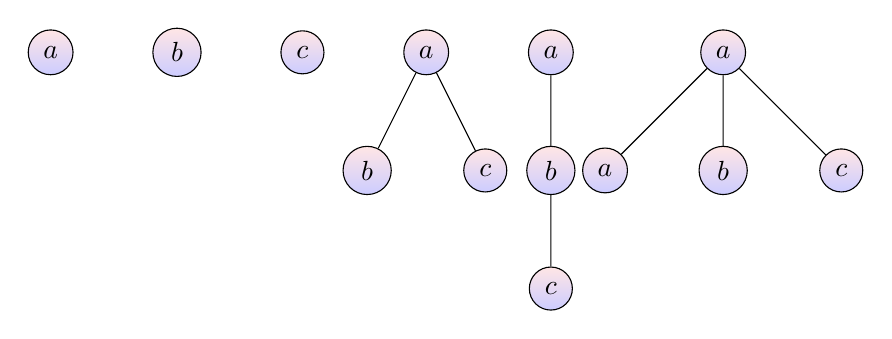
\begin{tikzpicture}[every node/.style={shape=circle, draw, align=center,
          top color=red!10, bottom color=blue!20}]
    \usetikzlibrary{trees,chains}
    \begin{scope}[start chain=growing right]
      \node[on chain]{$a$};
      \node[on chain]{$b$};
      \node[on chain]{$c$};
      \node[on chain]{$a$} child{node{$b$}} child{node{$c$}};
      \node[on chain]{$a$} child{node{$b$} child{node{$c$}}};
      \node[on chain,xshift=4ex]{$a$}child {node{$a$}} child {node{$b$}} child{node{$c$}};
    \end{scope}
  \end{tikzpicture}
  \כיתוב{העצים~$a, b, c, a(b,c), a(b(a),a(a,b,c))∈T(❴⌘a, ⌘b, ⌘c❵$}
\end{figure}

§ חתימות וביטויים פורמליים

אנו רואים באיור שמספר הבנים של צומת המכיל את האות~$a$ אינו קבוע. בחלק מהעצים
לצומת זה אין בנים כלל, ואילו בעצים אחרים יש לצומת זה בן אחד, שני בנים, ואף
שלושה. כדי להגדיר עצים שבהם לכל צומת מסוג מסויים יש תמיד מספר בנים, נזדקק למושג
החתימה.

\החל{הגדרה}[חתימה] חתימה~$Γ$, הינה אלפאבית, (בדרך כלל סופי) עליו מוגדרת פונקצית
ערכיות~$\arity$ המתאימה לכל אות~$γ∈Γ$ מספר שלם אי שלילי,~$\arity:Σ→ℕ⁺$.
\גמר{הגדרה}
עבור חתימה~$Γ$, נסמן ב-$Γₙ$
את תת הקבוצה של איברי~$Γ$
שה-$\arity$ שלהם הוא~$n$
\begin{equation*}
  Γₙ=❴γ∈Γ\,|\,\arity(γ)=n❵.
\end{equation*}

ביטויים פורמליים מעל חתימה דומים לעצים מעל אלפאבית, בצירוף המגבלה שלצומת
המסומנת באות~$n_γ∈Γ$, יש בדיוק~$\arity(γ)$ בנים. פורמלית,

\החל{הגדרה}[ביטויים פורמליים מעל חתימה] בהנתן חתימה~$Γ$
  אזי,~$E(Γ)$,
  קבוצת הביטויים הפורמליים מעל~$Γ$
  מוגדרת באמצעות הבנאי ה-$n$ מקומי,

  \begin{equation*}
    \infer{σ(τ₁,⋯,τₙ)∈T(Γ)}{σ∈Σ & n≥0 &γ∈Γₙ&τ₁∈T(Γ) &⋯&τₙ∈T(Γ) }
  \end{equation*}
\גמר{הגדרה}
\פסקה{דוגמה: ביטויים סימבוליים כביטויים פורמליים}
בהינתן אלפאבית~$Σ$, נבנה ממנו חתימה~$Γ$ באופן הבא:
\begin{align*}
   & Γ=Γ₀∪Γ₂ ⏎
   & Γ₀=Σ ⏎
   & Γ₂=❴.❵
\end{align*}
קל לראות שהביטויים הפורמליים ב-$E(Γ)$ הם בדיוק בעלי אותו מבנה כמו הביטויים
הסימבוליים בקבוצה~$S)Σ$.

\פסקה{דוגמה: ביטויים חשבוניים}
נסתכל למשל על החתימה הבאה
\begin{equation}
  \begin{split}
    % & Γ=Γ₀∪Γ₁∪Γ₂ ⏎
    % & Γ₀=❰⌘0,⌘1,⌘2,⌘3,⌘4,⌘5,⌘6,⌘7,⌘8,⌘9❱^*⏎
    % &\quad=❴⌘0,⌘1,⌘2,…,⌘10,⌘11,…,⌘{100},⌘{101},…,⌘{1000},⌘{1001},…❵ ⏎
    % & Γ₁=❴⌘-,⌘!,⌘{$√$}❵ ⏎
    & Γ₂=❴⌘+,⌘*,⌘/❵
  \end{split}
\end{equation}
חתימה זז היא חתימה אינסופית בגודלה, שבה ה-arity של הסימנים~$⌘+$,~$⌘*$ ו-$⌘/$
הוא 2, ה-arity של הסימנים ⌘!,
ו-$⌘-$ הוא 1, וה-arity של קבוצת המספרים
הטבעיים הוא 0. קבוצת הביטויים מעל חתימה זו היא לא אחרת מאשר קבוצת הביטויים
החשבוניים הבנויים ממספרים הטבעיים, האופרטורים הבינאריים של חיבור, כפל וחילוק,
והאופטורים האונאריים של השלילה, העצרת, והוצאת השורש. כמה ביטויים בקבוצה זו
מודגמים באיור הבא:

\begin{figure}
  \centering
  \begin{tikzpicture}[every node/.style={shape=circle,
          draw, align=center,
          top color=red!10, bottom color=blue!20}]
    \begin{scope}[yshift=-10ex,start chain=growing right,minimum size=2em]
      \node[on chain,circle,draw]{⌘1};
      \node[on chain,circle,draw]{⌘0};
      \node[on chain,circle,draw]{⌘!} child {node {⌘3}};
      \node[on chain,circle,draw]{⌘!} child {node{⌘*} child{node{⌘a}} child{node{⌘-} child{node{42}}}};
      % \node[on chain,circle,draw,xshift=5ex]{⌘√{}}
      child {node{⌘/}
          child {node{5}}
          child {node{3}}
        }
      ;
    \end{scope}
  \end{tikzpicture}
\end{figure}

נשים לב שההגדרה במובן זה שהיא קובעת את מבנה העצים, ולא את המשמעות שלהם. אין שום
דבר בהגדרה הנותן משמעות של חיבור לסימן ה-+. ההגדרה גם אינה מעניקה משמעות לקבוצת
המספרים הטבעיים. לדידה של ההגדרה, מספר טבעי הוא סדרת ספרות
נטולת משמעות.

§ ביטויים רגולריים

ביטויים רגולריים הם מכשיר חשוב להגדרת שפות פורמליות מעל אלפאבית נתון. ביטויים
רגולריים דומים במבנה שלהם לביטויים חשבוניים: הם עצים, אשר בצמתים פנימיים נמצא
אופרטורים בעלי arity ידוע, כאשר בעלים נמצאים סימנים מתוך האלפאבית.

§§ ביטויים רגולריים כביטויים מעל חתימה
בהינתן אלפאבית~$Σ$, נבנה מעליו חתימה~$Γ$, כאשר~$Γ=Γ₀∪Γ₁∪Γ₂$ וכן
\begin{equation}
  \begin{split}
    Γ₀ &=Σ^* ⏎
    Γ₁ &=❴⌘*❵ ⏎
    Γ₂ &=❴⌘;,⌘|❵
  \end{split}
\end{equation}
נגדיר כעת את~$\RE(Σ)$ קבוצת הביטויים הרגולריים מעל האלפאבית~$Σ$ כקבוצת הביטויים מעל
החתימה~$Γ$,
\begin{equation}
  \RE(Σ)=E(Γ)
\end{equation}
עלים של ביטויים אלו הם מילים מהאלפאבית~$Σ$ ובכלל אלו המילה הריקה~$ε$. לצמתים
פנימיים המסומנים ב-⌘* יש בן אחד בדיוק. לצמתים פנימיים המסומנים ב-⌘; או ב-⌘| יש
שני בנים בדיוק.

\פנה{figure:regexp} מראה כמה ביטויים רגולריים הנבנים כביטויים מעל האלפאבית~$❴a,b,c❵$
\begin{figure}
  \centering
  \begin{tikzpicture}[every node/.style={shape=circle,
          draw, align=center,
          top color=red!10, bottom color=blue!20}]
    \usetikzlibrary{trees,chains}
    \begin{scope}[start chain=growing right,minimum size=2em]
      \node[on chain,circle,draw]{$⌘;$} child {node{$⌘*$} child{node{$⌘|$} child{node{$⌘a⌘b$}} child{node{$⌘c$}}}}
      child{node{$⌘*$} child{node{$⌘b$}}};
      \node[on chain,circle,draw,xshift=8ex]{$⌘*$}
      child {node{$⌘|$}
          child {node{$⌘a$}}
          child {node{$⌘|$} child{node{$ε$}} child{node{$⌘c$}}}
        }
      ;
    \end{scope}
  \end{tikzpicture}
  \כיתוב{ביטויים רגולריים כביטויים מעל החתימה~$Γ=Γ₀∪Γ₁∪Γ₂$, הכוללת את
  העלים~$Γ₀=❴⌘a, ⌘b, ⌘c❵^*$, האופראטור האונארי~$Γ₁=❴⌘*❵$ ושני האופראטורים
  הבינאריים,~$Γ₂=❴⌘;,⌘|❵$}.
  \label{figure:regexp}
\end{figure}

§§ קבוצת הביטויים הרגולריים כשפה פורמלית

בהגדרה לעיל, הצגנו את קבוצת הביטויים הרגולרים כסוג של עצים מעל חתימה שנבנתה מעל
אלפאבית נתון. אולם, ניתן להציג את קבוצת הביטויים הרגולריים באופן ישיר כשפה
פורמלית מעל אלפאבית אותו הרחבנו באמצעות תוספת של סימני פיסוק מתאימים

\החל{הגדרה}[ביטויים רגולריים כשפה פורמלית]
  \label{definition:re}
  בהנתן אלפאבית~$Σ$ אזי,~$\RE(Σ)$, \עבה{השפה הפורמלית של הביטויים הרגולריים
  מעל~$Σ$}, היא שפה פורמלית מעל האלפאבית המורחב~$Σ∪❴⌘|,⌘*, ⌘), ⌘(❵$ (כאשר אנו מניחים
  כי $⌘|,⌘*,⌘),⌘(∉Σ$( כלומר \[
    \RE(Σ) ⊂❨Σ∪❴⌘|,⌘*,⌘),⌘(❵❩^*
\] אשר מוגדרת באמצעות ארבעה כללי היסק,
    \begin{align}
       & \infer{r∈\RE(Σ)}{r∈Σ^*} ⏎
       & \infer{(r₁⌘|r₂)∈\RE(Σ)}{r₁∈S(Σ) & r₂∈\RE(Σ)} ⏎
       & \infer{(r₁r₂)∈\RE(Σ)}{r₁∈S(Σ) & r₂∈\RE(Σ)} ⏎
       & \infer{(r*)∈\RE(Σ)}{r∈\RE(Σ)}. 
    \end{align}
\גמר{הגדרה}

§§ המשמעות של ביטויים רגולריים
בכדי לתת משמעות לשפה הפורמלית של הביטויים הרגולריים, נגדיר פונקצית משמעות
המייחסת לכל ביטוי רגולרי מעל~$Σ$ משמעות. כדי להבחין בין ביטוי רגולרי שהוא מילה
מעל~$Σ'$, ובין המשמעות של הביטוי, נשתמש ב-$r$ לציון הביטוי הרגולרי כמילה, וב-$⟦r⟧$ לציון
משמעות המילה.

\פסקה{סיכום}
בכדי לחדד את ההבדלים בין מילה ובין משמעותה,
נסכם את הסימונים שבהם השתמשנו עד כה, ואת יחסי ההכלה ביניהם:
\אבגד
✦ \mbox{$Σ$}. \quad
האלפאבית הנתון, למשל~$Σ=❴a,b,c❵$.
✦ \mbox{$r∈\RE(Σ)$}. \quad
הסימון~$r$ מתייחס למילה בשפה הפורמלית~$\RE(Σ)$, ולא למשמעות המילה.
✦ \mbox{~$\RE(Σ)⊆❨Σ'❩^*$}. \quad
הקבוצה~$\RE(Σ)$ היא שפה פורמלית מעל האלפאבית~$Σ'$.
✦ \mbox{~$Σ'=Σ∪❴;,),(,|,*❵$}. \quad
האלפאבית~$Σ'$ מתקבל מהאלפאבית המקורית בתוספת חמישה סימני פיסוק שלא היו בו.
✦ \mbox{~$⟦r⟧⊆Σ^*$}. \quad
הסימון
$⟦r⟧$ מתייחס להמשמעות של המילה~$r$, שהיא קבוצה של מילים מעל האלפאאבית הנתון~$Σ$.
✦ \mbox{$⟦r⟧∈℘Σ^*$}. \quad
$⟦r⟧$ שייכת לקבוצת הפשות הפורמליות מעל~$Σ$.
✦ \mbox{$⟦·⟧:\RE(Σ)→℘Σ^*$}.\quad
הפונקציה~$⟦·⟧$, כפונקציה של ארגומנט אחד, היא פונקציה מהשפה הפורמלית~$\RE(Σ)$
(שפה אשר מוגדרת מעל האלפאבית המורחב~$Σ'$) אל קבוצת השפות הפורמליות מעל~$Σ$ (האלפאבית המקורי).
✦ \mbox{$⟦·⟧:❨Σ'❩^*⇸℘Σ^*$}.\quad
הפונקציה~$⟦·⟧$ היא פונקציה חלקית מקבוצות המילים מעל האלפאבית המורחב, אל קבוצת
השפות הפורמליות מעל~$Σ$ (האלפאבית המקורי). הפונקציה היא חלקית, כי לא כל מילה
הכתובה באלפאית~$Σ'$, היא ביטוי רגולרי חוקי, כלומר ניתנת להתקבל באמצעות
ההגדרה
\פנה{definition:regular}.
===
גם הגדרת~$⟦r⟧$, פונקצית המשמעות של ביטוי רגולרי היא רקורסיבית, ורקורסיה זו תואמת את הרקורסיה שבהגדרה
\פנה{definition:re}.

\גמר{הגדרה}[ביטויים רגולריים כשפה פורמלית]
  \label{definition:regular}
  בהינתן ביטוי רגולרי~$r$, כללי ההיסק הבאים קובעים את משמעותו~$⟦r⟧$
  ⌘החל{ספרור}
  ✦ \mbox{} \[
    \infer{⟦r⟧=❴r❵}{r∈Σ^*}
\] כלומר, המשמעות של ביטוי רגולרי שהוא מילה מעל~$Σ$ היא השפה הפורמלית המכילה מילה זו בלבד.
  ✦ \mbox{} \[
    \infer{⟦(r₁|r₂)⟧=⟦r₁⟧∪⟦r₂⟧}{r₁∈\RE(Σ) & r₂∈\RE(Σ)}
\] אם~$r₁$ ו-$r₂$ הם ביטויים רגולריים, אזי~$⟦(r₁|r₂)⟧$, המשמעות של~$(r₁|r₂)$, היא הקבוצה המתקבלת מאיחוד הקבוצות שהן המשמעות של~$r₁$ ושל~$r₂$.
  ✦ \mbox{} \[
    \infer{⟦(r₁;r₂)⟧=❴w₁w₂\,|\,w₁∈⟦r₁⟧∧w₂∈⟦r₂⟧❵}{r₁∈\RE(Σ) & r₂∈\RE(Σ)}
\] אם~$r₁$ ו-$r₂$ הם ביטויים רגולריים, אזי~$⟦(r₁;r₂)⟧$, המשמעות של~$(r₁|r₂)$, היא הקבוצה המתקבלת מכל המילים שאפשר לחלק אותן לשתי מילים עוקבות, כך שהאחת נמצאת בתוך השפה שהיא המשמעות של הביטוי~$r₁$ ואילו המילה האחרת נמצאת בתוך השפה הפורמלית שהיא המשמעות של הביטוי~$r₂$.
  ✦ \mbox{} \[
    \infer
    {⟦(r*)⟧=⟦ε⟧∪⟦r⟧∪⟦(r;r)⟧∪⟦(r;(r;r))⟧∪
    ⋯∪⟦(r;(r;⋯(r;r)⋯)∪⋯⟧
    }{r∈\RE(Σ)}
\] אם~$r$ הוא ביטוי רגולריים, אזי~$⟦(r*)⟧$, המשמעות של~$(r*)$, היא הקבוצה המתקבלת מכל המילים שאפשר לחלק אותן ל-$n≥0$ מילים עוקבות שכל אחת מהן לקוחה מתוך~$⟦r⟧$, השפה הפורמלית המוגדרת על ידי~$r$.
  ⌘גמר{ספרור}
\גמר{הגדרה}

\פסקה{דוגמאות}
הביטוי הרגולרי \[
  (a);((a|(b|c)))*);(c)
\] מציין את השפה~$L₃$, השפה של כל המילים המתחילות באות~$a$ ומסתיימות באות~$c$ \[
  ⟦(a);((a|(b|c)))*);(c)⟧=L₃.
\] הביטוי הרגולרי \[
  ((((a)*);((b)*));((c*)))
\] מציין את השפה~$L₄$, שפת המילים שהאותיות שלהן מופיעות בסדר אלפאביתי לא יורד \[
  ⟦ (((a)*);((b)*));((c*))⟧=L₄.
\] §§ כתיב מקוצר לביטויים רגולריים
הכתיב שהוצע ב\פנה{definition:re} הוא ארכני, שכן כל הפעלה של בנאי מוסיפה זוג של סוגריים לביטוי. נהוג להשתמש בכתיב מקוצר המסתמך על שלוש מוסכמות:
\ספרר
✦ יש שימו באסוציאטיביות של ⌘| ⌘; כדי להשמיט סוגריים. כך למשל, במקום
$(a|(b|c))$
כותבים בקיצור
$(a|b|c)$
✦ כללי קדימות, לפיהם הסימן \* הוא בעל הקדימות הגבוהה ביותר, והסימן ⌘| בעל הקדימות הנמוכה ביותר מאפשרים להשמיט סימני סוגריים נוספים. כך למשל, במקום
$(a*);(b*)$
נכתוב~$a*b*$.

✦ סימן השרשור (⌘;) מושמט. במקום
$a;b;c$
נכתוב בקיצור~$abc$.

====בכתיב זה הביטוי הרגולרי המתאר את השפה~$L₄$ נכתב כ-
$a*b*c*$.
עוד נהוג שלא להקפיד על ההבדלה בין הביטוי כמילה, ובין המשמעות שלו, ולכן, בדרך כלל כותבים בקיצור
$L₄=a*b*c*$
במקום
$L₄=⟦a*b*c*⟧$.
בכתיב המקוצר, הביטוי הרגולרי~$(a|c)(a|c)(a|c)(a|c)(a|c)*$ מתאר את השפה
השפה~$L₅$ המכילה את כל המילים בנות חמש אותיות או יותר שאף אחת מהן אינה האות ⌘b.

ישנם כלים רבים המאפשרים לבצע חיפוש והחלפה בטקסט תוך שימוש בביטויים רגולריים. כלים אלו מוסיפים קיצורים משלהם, אך כמה קיצורים מופיעים באורח זהה כמעט בכל כלי המאפשר למשתמש בו להגדיר ביטויים רגולריים.
\ספרר

✦ עבור~$σ₁,σ₂,…σₖ∈Σ$, הסימון
$[σ₁σ₂⋯σₖ]$
הוא קיצור לביטוי
$(σ₁|σ₂|⋯|σₖ)$
כלומר, ביטוי המתאים לכל מילה שהיא תו אחד בדיוק מבין
$σ₁,σ₂,…,σₖ$.
כך למשל ⌘{+|-}
יכתב כ-⌘{[+-]}.

✦ אם~$r$ הוא ביטוי רגולרי, אזי~$r?$ הוא קיצור לביטוי הרגולרי~$(r|ε)$. כך למשל
השפה המתאימה לביטוי הרגולרי ⌘{?[+-]} מכילה שלוש מילים~$❴ε, ⌘a, ⌘b❵$.

✦ אם~$r$ הוא ביטוי רגולרי, אזי~$r+$ הוא קיצור לביטוי הרגולרי~$rr*$, כלומר מילה
המכילה מופע אחד או יותר של~$r$.

✦ בהנחה שיש סדר מוסכם של התווים באלפאבית~$Σ$, הסימון~$σ₁-σ₂$ כשהוא מופיע בתוך
סוגריים מרובעים, הוא קיצור של רשימת כל התווים בין~$σ₁$ ובין~$σ₂$.
כך למשל הביטוי הרגולרי
\begin{quote}
  ⌘{[0-9]+}
\end{quote}
מתאר סדרה לא ריקה של ספרות עשרוניות, ואילו
\begin{quote}
  ⌘{[-+]?[0-9]+}
\end{quote}
הסימן "." (נקודה) מתאר את הביטוי הרגולרי שמכיל אות אחת בדיוק מהאלפאבית.
====

בהינת אלפאבית~$Σ$ של סימנים יסודיים, נגדיר כ-$Σ^*$ את אוסף כל הסדריות (Strings) הסופיות שניתן לכתוב בעזרתו, ובכלל אלו את הסדרית הריקה אשר מסומנת בדרך כלל כ-𝜺. במנוחים אלו שפה פורמלית היא פשוט תת-קבוצה של~$Σ*$ ביטויים רגולריים (regular expressions), הם מכשיר להגדרת שפות פורמליות.
קבוצת הביטויים הרגולריים מעל~$Σ$ מוגדרת רקורסיבית באופן הבא:
ביטויים אטומים:
כל תו ב-$Σ$ הוא ביטוי רגולרי אטומי המתאר שפה המכילה סדרית אחת בלבד, התו עצמו.
הסימן 𝜺 הוא ביטוי רגולרי אטומי, המתאר שפה המכילה את הסדרית הריקה בלבד.
כללי יצירה
אם R1 וְ ּR2 הם ביטוייים רגולריים, אזי
R1R2 הוא ביטוי רגולרי שהשפה שלו מורכבת מכל הסדריות שאפשר לחלק אותם לשני חלקים רצופים וזרים, כאשר החלק הראשון, הרישא של הסדרית, שייך לשפה של R1 ואילו החלק השני, הסיפא, שייך לשפה של R2.
R1 | R2 הוא ביטוי רגולרי שהשפה שלו היא האיחוד של שתי השפות של R1 וְ R2.
אם ּR הוא ביטוי רגולרי, אזי גם+R הוא ביטוי רגולרי, שהשפה שלו היא כל הסדריות שניתן לחלק אותן לסדריות זרות ורצופות אשר כל אחת מהן שייכת לשפה של הביטוי הרגולרי R.
במרבית השימושים בפועל מוסיפים תַּחְבִּירִי סֻכָּר כגון:
?ּR הוא קיצור עבור R|𝜺
*R xהוא קיצור עבור (+R)|𝜺

ניתן לקצר את הכתיבה באמצעות מתן שמות לביטויים רגולריים חלקיים.
הנה דוגמא לשימוש ב-תַּחְבִּירִי סֻכָּר כדי להגדיר ביטוי רגולרי בעבור מזהה חוקי בִּשְׂפַת C:
\begin{verbatim}
Digit=0-9
Lower=a-z
Upper=A-Z
Letter=Lower|Upper
IdLetter=Letter|\$|\_
IdCharacter=IdLetter|Digit
Identifier=CLetter IdCharacter*
\end{verbatim}

כדאי לדעת כי ניתן לכתוב ביטוי רגולרי עבור חיתוך של השפות של שני ביטויים
רגולרייים, וגם עבור השפה של כל הסדריות של ביטוי רגולרי אחד אשר אינן מצויות בשפה
של ביטוי רגולרי אחר, וזאת בעבור כל שני ביטויים רגולריים שרירותיים. השימוש
בביטויים רגולריים בתיאור הדקדוק של שפה, אינו חשוב רק למען הדיוק. ישנם כלים
אוטומטיים אשר הקלט שלהם הוא ביטוי רגולרי ואשר מיייצרים תכניות המסוגלות לזהות
מופעים של ביטויים רגולריים בטקסט. כלים אלו מועילים מאוד בביטויים בכתיבת מהדרים
עבור שפות תכנות.בהינת אלפאבית~$Σ$ של סימנים יסודיים, נגדיר כ-$Σ*$ את אוסף כל הסדריות (Strings) הסופיות שניתן לכתוב בעזרתו, ובכלל אלו את הסדרית הריקה אשר מסומנת בדרך כלל כ-𝜺. במנוחים אלו שפה פורמלית היא פשוט תת-קבוצה של~$Σ*$ ביטויים רגולריים (regular expressions), הם מכשיר להגדרת שפות פורמליות.
קבוצת הביטויים הרגולריים מעל~$Σ$ מוגדרת רקורסיבית באופן הבא:
ביטויים אטומים:
כל תו ב-$Σ$ הוא ביטוי רגולרי אטומי המתאר שפה המכילה סדרית אחת בלבד, התו עצמו.
הסימן 𝜺 הוא ביטוי רגולרי אטומי, המתאר שפה המכילה את הסדרית הריקה בלבד.
כללי יצירה
אם R1 וְ ּR2 הם ביטוייים רגולריים, אזי
R1R2 הוא ביטוי רגולרי שהשפה שלו מורכבת מכל הסדריות שאפשר לחלק אותם לשני חלקים רצופים וזרים, כאשר החלק הראשון, הרישא של הסדרית, שייך לשפה של R1 ואילו החלק השני, הסיפא, שייך לשפה של R2.
R1 | R2 הוא ביטוי רגולרי שהשפה שלו היא האיחוד של שתי השפות של R1 וְ R2.
אם ּR הוא ביטוי רגולרי, אזי גם+R הוא ביטוי רגולרי, שהשפה שלו היא כל הסדריות שניתן לחלק אותן לסדריות זרות ורצופות אשר כל אחת מהן שייכת לשפה של הביטוי הרגולרי R.
במרבית השימושים בפועל מוסיפים תַּחְבִּירִי סֻכָּר כגון:
?ּR הוא קיצור עבור R|𝜺
*R הוא קיצור עבור (+R)|𝜺
u-v הוא קיצור עבור כל התווים שמצויים בין התווים u ל-v, תוך הנחה שיש סדר מוסכם של התווים באלפאבית~$Σ$
הסימן "." (נקודה) מתאר את הביטוי הרגולרי שמכיל אות אחת בדיוק מהאלפאבית.
ניתן לקצר את הכתיבה באמצעות מתן שמות לביטויים רגולריים חלקיים.
הנה דוגמא לשימוש ב-תַּחְבִּירִי סֻכָּר כדי להגדיר ביטוי רגולרי בעבור מזהה חוקי בִּשְׂפַת C:

כדאי לדעת כי ניתן לכתוב ביטוי רגולרי עבור חיתוך של השפות של שני ביטויים
רגולרייים, וגם עבור השפה של כל הסדריות של ביטוי רגולרי אחד אשר אינן מצויות בשפה
של ביטוי רגולרי אחר, וזאת בעבור כל שני ביטויים רגולריים שרירותיים. השימוש
בביטויים רגולריים בתיאור הדקדוק של שפה, אינו חשוב רק למען הדיוק. ישנם כלים
אוטומטיים אשר הקלט שלהם הוא ביטוי רגולרי ואשר מיייצרים תכניות המסוגלות לזהות
מופעים של ביטויים רגולריים בטקסט. כלים אלו מועילים מאוד בביטויים בכתיבת מהדרים
עבור שפות תכנות.

§§ שימוש בביטויים רגולריים בשפות תכנות.
§ דקדוקים
אוסף השפות הפורמליות הניתנות להגדרה על ידי ביטויים רגולריים הוא מוגבל.

דקדוק חסר הקשר הוא

\גמר{הגדרה}
  דקדוק חסר הקשר~$G$ הוא רביעיה~$G=⟨V,Σ,R,S⟩$
  כאשר~$V$ היא קבוצה של \עבה{משתנים}, הקרויים גם
  V is called a nonterminal character or a variable. Each variable represents a
  different type of phrase or clause in the sentence. Variables are also
  sometimes called syntactic categories. Each variable defines a sub-language
  of the language defined by G.  Σ is a finite set of terminals, disjoint from
  V, which make up the actual content of the sentence. The set of terminals is
  the alphabet of the language defined by the grammar G.
  R is a finite relation from V to {\displaystyle (V∪Σ)^*}(V∪Σ)^*, where the
  asterisk represents the Kleene star operation. The members of R are called
  the (rewrite) rules or productions of the grammar. (also commonly symbolized
  by a P) S is the start variable (or start symbol), used to represent the
  whole sentence (or program). It must be an element of V.
\גמר{הגדרה}

\החל{דוגמה}[שפת הסוגריים]
  $Σ=❴⌘(, ⌘)❵$,~$N=❴S❵$
  \begin{equation}
    \label{eq:parenthesis}
    \begin{split}
      S &→ε ⏎
      S &→(S) ⏎
      S&→SS ⏎
    \end{split}
  \end{equation}
\גמר{דוגמה}

\החל{דוגמה}[שפת הפלינדרומים]
  $Σ=❴⌘a, ⌘b, ⌘c❵$,~$N=❴S❵$
  \begin{equation}
    \label{eq:parenthesis}
    \begin{split}
      S &→ε ⏎
      S &→aSa ⏎
      S &→bSb ⏎
      S &→cSc
    \end{split}
  \end{equation}
\גמר{דוגמה}

\החל{דוגמה}[שפת הפונקציות הרציונליות]
  \label{example:rationals}
  $❴⌘1, ⌘I, ⌘(, ⌘), ⌘/, ⌘*, ⌘+, ⌘-❵$ \cref{eq:Q:alphabet}
  \begin{equation}
    \label{eq:parenthesis}
    \begin{split}
      S &→⌘1 ⏎
      S &→⌘I ⏎
      S &→⌘) -S ⌘(⏎
      S &→⌘)S ⌘+S⌘(⏎
      S &→⌘)S ⌘* S⌘(⏎
    \end{split}
  \end{equation}
\גמר{דוגמה}

\החל{דוגמה}[הדקדוק של שפת הביטויים הרגולריים]
  \label{example:grammar:re}
$\RE(Σ)$, השפה הפורמלית של הביטויים הרגולריים  
מעל אלפאבית~$Σ$ כפי שהוגדרה  באמצעות כללי היסק
ב\פנה{definition:re} ניתנת להגדרה גם באמצעות דקדוק 
  מעל~$Σ$}, 
  $Σ=❴σ₁,σ₂,…,σₙ❵$
  $❴σ₁,σ₂,…,σₙ, ⌘|, ⌘;, ⌘*, ⌘(, ⌘)❵$
  \begin{equation}
    \label{eq:parenthesis}
    \begin{split}
      R &→⌘(R ⌘*⌘) ⏎
      R &→⌘(R ⌘; R⌘) ⏎
      R &→⌘(R ⌘| R⌘) ⏎
      R &→ε⏎
      R &→σ₁ ⏎
      R &→σ₂ ⏎
      ⋮ ⏎
      R &→σₙ
    \end{split}
  \end{equation}
\גמר{דוגמה}

\endinput
במרבית השימושים בפועל מוסיפים תַּחְבִּירִי סֻכָּר כגון:

"לענין חוק זה, "יהודי" - מי שנולד לאם יהודיה או שנתגייר, והוא אינו בן דת אחרת".
אנו רואים שהגדרת מיהו יהודי לצורך חוק השבות היא רקורסיבית, שכן הגדרת המונח
"יהודי" בחוק מבוססת על המונח "יהודי" עצמו. אנו נאמר על קבוצה שהיא "קבוצה
מוגדרת רקורסיבית", אם היא מוגדרת באופן רקורסיבי שכזה. כלומר אפשר לחזור ולוהסיף
איברים לקבוצה אם הם נוצרים באופן מסוים מאיברים אחרים שהם כבר בקבוצה. יתירה מכך,
טבעה של הרקורסיה הוא שאפשר לחזור ולהפעיל אותה מספר בלתי חסום של פעמים.

כשמדברים על קבוצות מוגדרות רקורסיבית נוח להשתמש בכמה מונחים מוסכמים: איברים
אטומיים איברים מורכבים בנאים קל מאוד להבין אינטואיטיבית מהי קבוצה מוגדרת
רקורסיבית. גם פשר המונחים האלו הוא קל. די להציץ בדוגמאות אחדות כדי לגלות את
התבנית החוזרת. כיוון שקשה הרבה יותר להגדיר בצורה מדויקת את המונחים, נתחיל בכמה
דוגמאות.

כך לדוגמא, קבוצת ה\ביטויים היכולים להפיע בשפת תכנות כגון שפת פשוטה היא קבוצה
המוגדרת רקורסיבית: ה\ביטויים האטומיים הם הם מילולונים וקריאת ערכם שֶׁל \משתנים.
ביטויים מורכבים נוצרים מביטויים אחרים, היכולים להיות ביטויים יסודיים, או
ביטויים מורכבים אחרים, באמצעות מגוון שֶׁל פעולות, הכוללות, בין השאר, את פעולות
החשבון וקריאות לפונקציה.

איבר מקבוצה המוגדרת רקורסיבית הוא איבר אטומי אם לא ניתן לזהות בתוכה
תת-איברהשייכת לאותה קבוצה. חשוב להבין כי איבראטומית אינה בהכרח לא פריקה,
כל שנדרש הוא שלא ניתן לזהות בתוכה תת-איברמאותה קבוצה.

הנה, קבוצת הפקודות
במרבית שפת תכנות היא קבוצה המוגדרת רקורסיבית, ובתוך קבוצה זו, אנו יכולים לזהות
את הפקודות האטומיות. בשפת פסקל, \הצבה היא \פקודה אטומית. אבל, אם נעיין ב\פקודה
\החל{קוד}
\pascal{a :=b+c;}
\סוף{קוד}
שהיא \פקודה אטומית, נוכל לזהות בה תתי מרכיבים, למשל הביטוי \קד{b+c}. בכל זאת,
הפקודה לעיל היא פקודה פרימטיבית, שכן לא ניתן לזהות בה תת-מרכיב שהוא
\פקודה בעצמו.

לעומת זאת, ה\פקודה הבאה בפסקל,
\החל{PASCAL}
begin
a :=b+c;
end
\end{PASCAL}

אינה פקודה אטומית, שכן ניתן לאתר בה מרכיב שהוא \פקודה בעצמו.

קבוצת ה\טיפוסים שֶׁל שפת \סי (כמו גם קבוצת הטיפוסים שֶׁל שפת פסקל) אף היא קבוצה
המוגדרת רקורסיבית: ישנם טיפוסים מורכבים, אשר ניתן לזהות כי הם מורכבים מיחידות
קטנות יותר, אשר אף הן טיפוסים. בטיפוס רשומה למשל ניתן לזהות כיחידות
קטנות יותר את טיפוסי השדות הבונים את הרשומה. אנו אומרים שהטיפוס שֶׁל רשומה
הוא \מונח{טיפוס מורכב}, משום שיש בו תתי-יחידות אשר אף הן טיפוסים.

לעומת ה\מונח[טיפוס מורכב]{טיפוסים המורכבים}, ישנם טיפוסים אטומיים, כלומר
טיפוסים אשר לא ניתן לזהות בתוכם טיפוסים אחרים. הטיפוס שֶׁל מספרים שלמים או
הטיפוס שֶׁל מספרים ממשיים, הם דוגמאות לטיפוסים כאלו.

המילה השמורה \מש{int} בשפת \סי \מזהה את הטיפוס האטומי שֶׁל מספר שלם.
מילים
שמורות המשמשות כ\מזהים נקראות \מונח{מזהה שמור}.

ניתן להשתמש בשיטת ההגדרה הרקורסיבית, כדי להגדיר את קבוצת הפקודות בפסקל,

\החל{ספרור}
✦ \עבה{פקודות אטומיות} פקודות אטומיות הן פקודות שאינן בנויות מפקודות אחרות. בשפת \סי יש שני סוגים של פקודות אטומיות,
\החל{ספרור}
✦ \עבה{פקודה ריקה} פקודה שאינה מבצעת דבר, נקראת הפקודה הריקה. הפקודה הריקה נכתבת בשפת אמצעות סימן הנקודה ופסיק~\cc{;}
✦ \עבה{פקודת ביטוי} בשפת \סי, כל ביטוי שאחריו מופיע סימן הנקודה ופסיק~\cc{;}
\begin{CPP}
  a; f(); b=2; 2;++i; 1-1;
\end{CPP}
\סוף{ספרור}
קריאה לפרוצדורה
כללי היצירה העיקריים של הפקודות הם:
שרשור של פקודות המופרדות על ידי סימן הנקודה ופסיק (;) הוא פקודה.
פקודת תנאי, כפי שתוארה לעיל, היא פקודה, אשר מכילה בתוכה פקודה אחת או שתיים.
פקודת תנאי רבת ראשים המוגדרת באמצעות המילה השמורה case
לולאות המתארות ביצוע איטרטיבי של פקודה (אטומית או מורכבת), אף הן פקודות. יש בְּPascal שלושה סוגים של פקודות לולאה מורכבות:
for
while
repeat until
\סוף{ספרור}

3.3.2
​3.3.3​ קבוצת הפקודות בְּPascal היא קבוצה מוגדרת רקורסיבית
האיברים האטומיים, הלא הם הפקודות האטומיות, הם שלושה:
הפקודה הריקה
פקודת ההצבה
קריאה לפרוצדורה
נשתמש בשיטה זו כדי להגדיר את אוסף הפקודות בְּPascal. האיברים האטומיים, הלא הם הפקודות האטומיות, הם שלושה:
הפקודה הריקה
פקודת ההצבה
קריאה לפרוצדורה
כללי היצירה העיקריים של הפקודות הם:
שרשור של פקודות המופרדות על ידי סימן הנקודה ופסיק (;) הוא פקודה.
פקודת תנאי, כפי שתוארה לעיל, היא פקודה, אשר מכילה בתוכה פקודה אחת או שתיים.
פקודת תנאי רבת ראשים המוגדרת באמצעות המילה השמורה case
לולאות המתארות ביצוע איטרטיבי של פקודה (אטומית או מורכבת), אף הן פקודות. יש בְּPascal שלושה סוגים של פקודות לולאה מורכבות:
for
while
repeat until
ניתן גם באופן דומה להגדיר את הביטויים בִּשְׂפַת תכנות פשוטה. הביטויים האטומיים יהיו מספרים ושמות משתנים, ואילו כללי היצירה יהיו מבוססים על פעולות החשבון וסימני הסוגריים.
​3.3.4​ דקדוקי עניות במונח "קבוצה מוגדרת רקורסיבית"
יוזהר מראש כי ההגדרה הפורמלית הזו של המונחים שבהם השתמשנו היא מסורבלת. למרבה המזל, אף כי יש חשיבות מסוימת לדקדוקי העניות אלו, ההבנה האינטואטיבית חשובה יותר.
בכל הגדר רקורסיבית של קבוצה יש שלושה מרכיבים.
רשימה של איברים אטומיים אשר משתייכים לקבוצה בכוח עצמם בלבד.
נסתכל לרגע על קבוצת הטיפוסים בִּשְׂפַת פסקל. קבוצה זו היא קבוצה מוגדרת רקורסיבית, בקבוצה זו ישנם ארבעה איברים אטומיים מסוג זה: Character, Integer, Real, Boolean. כל שאר הטיפוסים נוצרים באמצעות בנאים.
רשימה של בנאים.
בנאי הוא פונקציה שמקבלת פרמרטים שיכולים להיות:
אפס או יותר איברים של הקבוצה
אפס או יותר ערכים שאינם איברים של הקבוצה.
ומחזירה ערך שאף הוא בקבוצה.
איבר מורכב הוא איבר שנוצר מבנאי שקיבל כפרמטר איבר אחד לפחות של הקבוצה.
מערכים בִּשְׂפַת Pascal הם טיפוסים מורכבים: בנאי המערך קיבל כפרמטר את טיפוס של תא במערך, והחזיר בתמורה את טיפוס המערך של תאים מאותו טיפוס.
איבר אטומי הוא איבר שנוצר מבנאי שלא קיבל כפרמטרים ערכים של הקבוצה.
ניתן להסתכל על הטיפוסים אטומיים מכוח עצמם: Character, Integer, Real, Boolean כעל בנאים שאינם מקבלים פרמטרים כלל.
טיפוסים מנויים (enumerated types) בִּשְׂפַת פסקל, הם גם טיפוסים אטומיים (איברים אטומיים של קבוצת הטיפוסים) . הם נוצרו מבנאי שמקבלל רשימה של תגיות. תגית היא מזהה חוקי בִּשְׂפַת פסקל.
הדרישה, אשר למען הקיצור נוהגים להשמיטה, כי אין בקבוצה איברים אחרים פרט לאטומיים ולמורכבים שנוצרו באמצעות כללי היצירה. .
בדוגמה של חוק השבות, האיברים האטומיים הם אברהם אבינו, וחשוב מכך, שרה אמנו, וכל מי שנתגייר, ואילו היצירה הוא הלידה.
​3.3.5​ קבוצה שאינה מוגדרת רקורסיבית
נעיין לדוגמה בִּשְׂפַת MetaPost. שפה זו שייכת לפרדיגמה הדקלראטיבית. ליתר דיוק, השפה נועדה לשרטוט באמצעות אילוצים. המתכנת כותב רשימה של משוואות לינאריות, שהפתרון שלהן, שמחושב באופן אוטומטי על ידי מנוע הבנוי בשפה, קובע את השרטוט המבוקש.
במדריך של השפה קבוצת הטיפוסים מוגדרת באופן הבא:
MetaPost actually has ten basic data types: numeric, pair, path, transform, (rgb)color, cmykcolor, string, boolean, picture, and pen. Let us consider these one at a time beginning with the numeric type.
\החל{ציינון}
Numeric quantities in MetaPost are represented in fixed point arithmetic as
integer multiples of 165536, the smallest positive value, which is also
available as the predefined constant epsilon…

The pair type is represented as a pair of numeric quantities. We have seen that pairs are used to give coordinates in draw statements. Pairs can be added, subtracted, used in mediation expressions, or multiplied or divided by numerics…

A path represents a straight or curved line that is defined parametrically…

A transform can be any combination of rotating, scaling, slanting, and
shifting. If p=(𝑝𝑥, 𝑝𝑦) is a pair and T is a transform, p transformed T
is a pair of the form...
The color type is like the pair type, except that it has three components
instead of two and each component is normally between 0 and 1…The type
‘rgbcolor’ is an alias of type ‘color’. The cmykcolor type is similar to the
color type except that it has four components instead of three…

A string represents a sequence of characters…

The boolean type has the constants true and false and the operators and, or,
not…

The picture data type is just what the name implies. Anything that can be
drawn in MetaPost can be stored in a picture variable…Pictures can be added to
other pictures and operated on by transforms...

The main function of pens in MetaPost is to determine line thickness, but
they can also be used to achieve calligraphic effects. The statement a
~\cc{a}

\cc{pickup}$⟨${\itshape pen expression}$⟩$ causes the given pen to be used
in subsequent draw or drawdot statements...

\סוף{ציינון}
אנו רואים שבשפה ישנם טיפוסים מיוחדים שאינם שכיחים בשפות אחרות: עט, צבע, תמונה,
זוג, ועוד. אלא שהיחודיות הזו חסומה: אין אפשרות למתכנת בשפה להוסיף טיפוסים
חדשים. כיוון שקבוצת הטיפוסים היא קטנה וסופית, ברור שהיא אינה מוגדרת רקורסיבית,
שכן כל קבוצה מוגדרת רקורסיבית היא בלתי חסומה בגדלה. בפרט, אין בִּשְׂפַת MetaPost
בנאים או טיפוסים מורכבים. יש בה עשרה טיפוסים, ותו לא. כדאי להתעכב מעט על
הטיפוס pair: טיפוס זה אמנם מיוצג כזוג של numeric. אבל מדובר כאן בייצוג בלבד. לא
בבנית טיפוסים. אבל אין אפשרות ליצור זוג של שום טיפוס אחר. אין זוגות של תמונות,
צבעים, עטים, וגם אין זוגות של זוגות. יתירה מכך, יש פעולות יחודיות לזוג, כמו
טרנספורמציה שאינן נובעות מכך שהוא "מורכב" משני numeric. לפיכך, אין מדובר כאן
בבנאי של זוגות.

קבוצות מוגדרות רקורסיבית
רקורסיה אינה ענין של שפות תכנות בלבד
סעיף 4ב' לחוק השבות, תש"י - 1950 קובע:
"לענין חוק זה, "יהודי" - מי שנולד לאם יהודיה או שנתגייר, והוא אינו בן דת אחרת".†{הגדרה רקורסיבית דומה קיימת ביחס לשאלה "מיהו מוסלמי?". על פי ההלכה המוסלמית, מוסלמי הוא מי שנולד לאב מוסלמי, או שהפך למוסלמי באמצעות אמירת העדות, הלא היא השהאדה: لَا إِلٰهَ إِلَّا الله مُحَمَّدٌ رَسُولُ الله בפומבי. אבל, כיוון שהאמירה חייבת להעשות בפני מי שהם מוסלמים, ההתאסלמות מהווה כלל יצירה של איבר מורכב. אגב, ההמרה לנצרות, לפחות על פי כתבי הקודש דורשת גם היא אמירה, אך אמירה זו היא פרטית ולא פומבית, ככתוב באיגרת פולוס השליח אל הרומיים, פרק י"א "כִּי אִם־בְּפִיךָ תוֹדֶה שֶׁיֵּשׁוּעַ הוּא הָאָדוֹן וְתַאֲמִין בִּלְבָבְךָ שֶׁהָאֱלֹהִים הֱעִירוֹ מִן־הַמֵּתִים תִּוָּשֵׁעַ׃ כִּי בִלְבָבוֹ יַאֲמִין הָאָדָם וְהָיְתָה לּוֹ לִצְדָקָה וּבְפִיהוּ יוֹדֶה וְהָיְתָה־לּוֹ לִישׁוּעָה׃ כִּי הַכָּתוּב אֹמֵר כָּל־הַמַּאֲמִין בּוֹ לֹא יֵבוֹשׁ׃ וְאֵין הַפְרֵשׁ בֵּין הַיְּהוּדִי לַיְּוָנִי כִּי אָדוֹן אֶחָד לְכֻלָּם".}
אנו רואים שהגדרת מיהו יהודי לצורך חוק השבות היא רקורסיבית, שכן הגדרת המונח "יהודי" בחוק מבוססת על המונח "יהודי" עצמו.
אנו נאמר על קבוצה שהיא "קבוצה מוגדרת רקורסיבית†{20}", אם היא מוגדרת באופן רקורסיבי שכזה. כלומר אפשר לחזור ולוהסיף איברים לקבוצה אם הם נוצרים באופן מסוים מאיברים אחרים שהם כבר בקבוצה. יתירה מכך, טבעה של הרקורסיה הוא שאפשר לחזור ולהפעיל אותה מספר בלתי חסום של פעמים.
כשמדברים על קבוצות מוגדרות רקורסיבית נוח להשתמש בכמה מונחים מוסכמים:
\החל{ספרור}
איברים אטומיים
2. איברים מורכבים
3. בנאים
\סוף{ספרור}
קל מאוד להבין אינטואיטיבית מהי קבוצה מוגדרת רקורסיבית. גם פשר המונחים האלו הוא קל. די להציץ בדוגמאות אחדות כדי לגלות את התבנית החוזרת. כיוון שקשה הרבה יותר להגדיר בצורה מדויקת את המונחים, נתחיל בכמה דוגמאות.
בנאים, איברים מורכבים, איברים אטומיים בחוק השבות
אם נעמיק ברקורסיה שבחוק השבות נגלה:
\החל{ספרור}
איברים מורכבים. חוק השבות קובע את הכלל הבא: אם אדם נולד לאם יהודיה, אזי הוא יהודו. כלל זה הוא בנאי., אשר מקבל פרמטר שהוא אם יהודי, יוצר איבר חדש בקבוצה. תהליך הלידה מיצר מהפרמטר איבר חדש של הקבוצה אותה אנו מגדירים. איבר בקבוצה שנוצר מאיבר אחר, נקרא איבר מורכב.
איברים אטומיים: עוד בנאי נמצא בקביעה "אם פלוני התגייר הרי הוא נחשב כיהודי", גם היא בנאי. כלל זהו הוא בדיוק בנאי. אפשר לנסח זאת כך: הבנאי שלפנינו מקבל "פרמטר".ותהליך הגיור הופך זה את הפרמטר ליהודי. המתגיירים הם היהודים האטומיים.

ניתן גם באופן דומה להגדיר את הביטויים בִּשְׂפַת תכנות פשוטה. הביטויים האטומיים יהיו מספרים ושמות משתנים, ואילו כללי היצירה יהיו מבוססים על פעולות החשבון וסימני הסוגריים.
§ דקדוקי עניות במונח "קבוצה מוגדרת רקורסיבית"
יוזהר מראש כי ההגדרה הפורמלית הזו של המונחים שבהם השתמשנו היא מסורבלת. למרבה המזל, אף כי יש חשיבות מסוימת לדקדוקי העניות אלו, ההבנה האינטואטיבית חשובה יותר.
בכל הגדר רקורסיבית של קבוצה יש שלושה מרכיבים.
רשימה של איברים אטומיים אשר משתייכים לקבוצה בכוח עצמם בלבד.
נסתכל לרגע על קבוצת הטיפוסים בִּשְׂפַת פסקל. קבוצה זו היא קבוצה מוגדרת רקורסיבית, בקבוצה זו ישנם ארבעה איברים אטומיים מסוג זה: Character, Integer, Real, Boolean. כל שאר הטיפוסים נוצרים באמצעות בנאים.
רשימה של בנאים.
בנאי הוא פונקציה שמקבלת פרמרטים שיכולים להיות:
אפס או יותר איברים של הקבוצה
אפס או יותר ערכים שאינם איברים של הקבוצה.
ומחזירה ערך שאף הוא בקבוצה.
איבר מורכב הוא איבר שנוצר מבנאי שקיבל כפרמטר איבר אחד לפחות של הקבוצה.
מערכים בִּשְׂפַת Pascal הם טיפוסים מורכבים: בנאי המערך קיבל כפרמטר את טיפוס של תא במערך, והחזיר בתמורה את טיפוס המערך של תאים מאותו טיפוס.†{למען השלמות יש לציין שבנאי המערך מקבל עוד שני פרמטרים, שהם קצוות המערך. ואפשר להפליג ולצין שבנאי של מערך רב מימדי מקבל מספר זוגות של פרמטרים כנ"ל.}
איבר אטומי הוא איבר שנוצר מבנאי שלא קיבל כפרמטרים ערכים של הקבוצה.
ניתן להסתכל על הטיפוסים אטומיים מכוח עצמם: Character, Integer, Real, Boolean כעל בנאים שאינם מקבלים פרמטרים כלל.
טיפוסים מנויים (enumerated types) בִּשְׂפַת פסקל, הם גם טיפוסים אטומיים (איברים אטומיים של קבוצת הטיפוסים) . הם נוצרו מבנאי שמקבלל רשימה של תגיות. תגית היא מזהה חוקי בִּשְׂפַת פסקל.
הדרישה, אשר למען הקיצור נוהגים להשמיטה, כי אין בקבוצה איברים אחרים פרט לאטומיים ולמורכבים שנוצרו באמצעות כללי היצירה. .
בדוגמא של חוק השבות, האיברים האטומיים הם אברהם אבינו, וחשוב מכך, שרה אמנו, וכל מי שנתגייר, ואילו היצירה הוא הלידה.
§ קבוצה שאינה מוגדרת רקורסיבית
נעיין לדוגמא בִּשְׂפַת MetaPost. שפה זו שייכת לפרדיגמה הדקלראטיבית. ליתר דיוק, השפה נועדה לשרטוט באמצעות אילוצים. המתכנת כותב רשימה של משוואות לינאריות, שהפתרון שלהן, שמחושב באופן אוטומטי על ידי מנוע הבנוי בשפה, קובע את השרטוט המבוקש.
במדריך של השפה קבוצת הטיפוסים מוגדרת באופן הבא:

MetaPost actually has ten basic data types: numeric, pair, path, transform, (rgb)color, cmykcolor, string, boolean, picture, and pen. Let us consider these one at a time beginning with the numeric type.
\החל{ספרור}
Numeric quantities in MetaPost are represented in fixed point arithmetic as integer multiples of, the smallest positive value, which is also available as the predefined constant epsilon…
The pair type is represented as a pair of numeric quantities. We have seen that pairs are used to give coordinates in draw statements. Pairs can be added, subtracted, used in mediation expressions, or multiplied or divided by numerics…
A path represents a straight or curved line that is defined parametrically…
A transform can be any combination of rotating, scaling, slanting, and shifting. If p=(𝑝𝑥, 𝑝𝑦) is a pair and T is a transform,
p transformed T
is a pair of the form...
The color type is like the pair type, except that it has three components instead of two and each component is normally between 0 and 1…The type ‘rgbcolor’ is an alias of type ‘color’.
The cmykcolor type is similar to the color type except that it has four components instead of three…
A string represents a sequence of characters…
The boolean type has the constants true and false and the operators and, or, not…
The picture data type is just what the name implies. Anything that can be drawn in MetaPost can be stored in a picture variable…Pictures can be added to other pictures and operated on by transforms...
. The main function of pens in MetaPost is to determine line thickness, but they can also be used to achieve calligraphic effects. The statement pickup~$⟨{pen expression}⟩$ causes the given pen to be used in subsequent draw or drawdot statements…

\סוף{ספרור}
אנו רואים שבשפה ישנם טיפוסים מיוחדים שאינם שכיחים בשפות אחרות: עט, צבע,
תמונה, זוג, ועוד. אלא שהיחודיות הזו חסומה: אין אפשרות למתכנת בשפה להוסיף
טיפוסים חדשים. כיוון שקבוצת הטיפוסים היא קטנה וסופית, ברור שהיא אינה
מוגדרת רקורסיבית, שכן כל קבוצה מוגדרת רקורסיבית היא בלתי חסומה בגדלה.
בפרט, אין בִּשְׂפַת MetaPost בנאים או טיפוסים מורכבים. יש בה עשרה טיפוסים, ותו
לא. כדאי להתעכב מעט על הטיפוס pair: טיפוס זה אמנם מיוצג כזוג של numeric.
אבל מדובר כאן בייצוג בלבד. לא בבנית טיפוסים. אבל אין אפשרות ליצור זוג של
שום טיפוס אחר. אין זוגות של תמונות, צבעים, עטים, וגם אין זוגות של זוגות.
יתירה מכך, יש פעולות יחודיות לזוג, כמו טרנספורמציה שאינן נובעות מכך שהוא
"מורכב" משני numeric. לפיכך, אין מדובר כאן בבנאי של זוגות.
§§שפות פורמליות לתיאור שפות תכנות
§§§ביטויים רגולריים

דקדוקי BNF
כוח הביטוי של ביטויים רגולריים הוא מוגבל ביותר. כך למשל, לא ניתן לבטא
באמצעות ביטוי רגולרי את הדרישה שהסוגריים בתכנית מאוזנים. לפיכך, השימוש
בביטויים
רגולריים מוגבל להגדרות פשוטות של אבני הבנין של השפה: משתנים, הערות, מספרים
וכו'. להגדרות מורכבות יותר, יש להשתמש במנגנון הידוע בשם דקדוק חסר הקשר
(Context Free Grammar), אשר נכתב בדרך כלל בשיטת הסימון הידועה בשם Backus Naur
Form או BNF. כתיב אחר לדקדוקים אלו הוא הדיאגרמות שתוארו לעיל.
הגדרת דקדוק בשיטת סימון זו מורכבת מארבעה חלקים:
\החל{ספרור}
קבוצה של סימנים סופיים, Terminals. (ה-Terminals קרויים
לעיתים גם Tokens או אסימונים). הדקדוק מתאר שפה מעל האלפאבית
שיוצרים הסימנים הסופיים.
קבוצה של סימנים לא סופיים, Non Terminal Symbols, המשמשים
ככלי עזר להגדרת הדקדוק. סימני עזר אלו דומים מעט לשימוש בשמות
לביטויים רגולריים חלקיים, אלא, שהגדרתם של סימני העזר הללו
יכולה להיות רקורסיבית, וניתן להגדירן יותר מאשר פעם אחת.
קביעה של אחד מהסימנים הלא סופיים כסימן התחלה: Start Symbol
אוסף של כללי גזירה, כאשר לכלל גזירה יש שני חלקים: ראש הכלל
הכתוב בצד שמאל של הכלל, הוא תמיד סימן לא סופי, ואילו גוף הכלל
הכתוב בצידו הימני, הוא סדרית (היכולה להיות ריקה) של סימנים
סופיים ולא סופיים. כללי הגזירה נכתבים כך שישנו חץ המוביל מראש
הכלל אל גופו. בפועל, נוהגים להשמיט את המרכיבים 1 עד 3 של
הגדרת הדקדוק ולהסתפק בכללי הגזירה לבדם. קל להבחין בין סימנים
סופיים ולא סופיים בכללי הגזירה, משום שסימן סופי לא יופיע
לעולם בראש כלל. גם סימן ההתחלה ברור בדרך כלל מההקשר.
\סוף{ספרור}
הנה דוגמא:
\begin{align}
  S &→E ⏎
  E &→a E b ⏎
  E &→𝜺 ⏎
\end{align}

בדוגמא זו בדקדוק ישנם שלושה כללי גזירה, אשר מקריאתם מתגלה כי:
\החל{ספרור}
הסימנים הלא סופיים הם S וְ E
סימן ההתחלה הוא S
הסימנים הלא סופיים הם a וְ b
\סוף{ספרור}
השפה המוגדרת על ידי הדקדוק חסר ההקשר הזה היא פשוטה ביותר, והיא מכילה את
כל הסדריות שבראשן יש מספר n (שיכול להיות 0) של a ואחריהם n מופעים של
הסימן b.
ניתן להוכיח (ולא נעשה זאת כאן), כי לא ניתן להגדיר שפה זו באמצעות ביטויים
רגולריים.

הנה דוגמא המהווה קטע של הדקדוק של שְׂפַת פסקל:

\begin{derivation}
  \begin{align}
    pascal-program→program identifier program-heading ; block . ⏎
    program-heading→𝜺 ⏎
    program-heading→(identifier-list) ⏎
    identifier-list→identifier ⏎
    identifier-list→identifier-list, identifier ⏎
    block→block1 ⏎
    block→label-declaration ; block1 ⏎
    block1→block2 ⏎
    block1→constant-declaration ; block2 ⏎
    block2→block3 ⏎
    block2→type-declaration ; block3 ⏎
    block3→block4 ⏎
    block3→variable-declaration ; block4 ⏎
    block4→block5 ⏎
    block4→proc-and-func-declaration ; block5 ⏎
    block5→begin statement-list end ⏎
  …⏎
    type-declaration→type type-declarator ⏎
    type-declaration→type-declaration ; type-declarator ⏎
    type-declarator→identifier=type ⏎
  …⏎
    type→identifier ⏎
    type→record field-list \=end=⏎
    field-list→𝜺 ⏎
  \end{align}
\end{derivation}

קל לזהות בהגדרת דקדוק זו את סימן ההתחלה. לשם הנוחות סימנו את הסימנים
הסופיים כגופן וצבע מיוחדים. מהגדרת הדקוק הזו אנו למדים למשל: \החל{ציינון}
תכנית Pascal מתחילה תמיד במילה program ומסתיימת בסימן ". "
לתכנית יש שם שאחריו יכולה להפועים רשימת מזהים העטופה בסוגריים עגולים.
בראש התכנית יש ארבעה פרקי הגדרות החייבים להופיע בסדר קבוע: הגדרת תוויות,
הגדרת קבועים, הגדרת טיפוסים והגדרת משתנים. כל אחד מארבעת מפרקי ההגדרות הוא
אופציונלי.
בהגדרת פרק הטיפוסים אם מופיעה המילה type אזי אחריה חייבת להופיע הגדרת טיפוס
אחת לפחות.
הגדרות הטיפוסים חייבות להיות מופרדות בסימן ";"
כל הגדרת טיפוס בודדת מכילה מזהה, סימן שיווין, ואחריו גוף הטיפוס, שיכול להיות מזהה או רשומה.
\סוף{ציינון}

והנה דוגמא לתכנית פשוטה (וסרת טעם) המצייתת לדקדוק לעיל:

\begin{verbatim}
program p;
type
shalem=integer;
student=record
end;
begin
end.
\end{verbatim}

הגדרת הדקדוק של שְׂפַת תכנות באמצעות דקדוק חסר הקשר לא נועדה למען הדיוק
בלבד. ישנם כלים אוטמטיים המאפשרים תרגום של דקדוק חסר הקשר כזה לתכנית
ניתוח, אשר לוקחת טכסט נתון, ובונה בעבורו את אופן גזירתו מהדקדוק. אופן
הגזירה הזה נקרא "עץ גזירה" (ַParse Tree) אשר מהווה הוכחה כי הטכסט אמנם
נגזר מהדקדוק. הפורמליזם של דקדוק BNF חזק יותר מהפורמליזם של ביטויים
רגולריים שכן הוא מתיר הגדרות רקורסיביות. כך למשל, בהגדרת הדקדוק של Pascal
נמצא הגדרות רקורסיביות שבהן הסימן הלא סופי statement-list מוגדר באמצעות
הסימן הלא סופי statement ולהיפך:

\begin{align}
  statement-list→statement
  statement-list→statement-list ; statement
  statement→𝜺
  statement→variable :=expression
  statement→begin statement-list end
  statement→if expression then statement
  statement→if expression then statement else statement
  statement→case expression of case-list end
  statement→while expression do statement
  statement→repeat statement-list until expression
  statement→for varid :=for-list do statement
  statement→procid
  statement→procid(expression-list)
  statement→goto label
  statement→with record-variable-list do statement
  statement→label : statement
\end{align}

הגדרות רקורסיביות מעין אלו הינן חיוניות בהגדרת שפות תכנות מודרניות, אך הן אינן
ניתנות להיעשות בביטויים רגולריים. דקדוקי EBNF EBNF הוא קיצור של Extended BNF.
פורמליזם זה דומה בעיקרו לפורמליזם של דקדוק BNF, אלא שגופו של כלל הגזירה יכול
להיות ביטוי רגולרי מעל אוסף הסימנים, הסופיים והלא סופיים כאחד. שימוש בביטויים
רגולריים כאלו הוא בבחינת תַּחְבִּירִי סֻכָּר לדקדוקי BNF. ההרחבה עצמה אינה מאפשרת
הגדרת שפות פורמליות נוספות פרט לאלו הניתנות להגדרה בדקדוק BNF, אך ניתן באמצות
הרחבה זו להגדיר שפות פורמליות ביתר תמציתיות.

הנה שכתוב של קטע הדקדוק הראשון של Pascal שהבאנו כאן, תוך שימוש בשיטות הסימון
של EBNF.

\begin{align}
  Pascal -program→program identifier [(identifier {,identifier})] ; block .
  block→[label-declaration;]
  [constant-declaration;]
  [type-declaration;]
  [variable-declaration ;]
  begin statement-list end
…
  type-declaration→type ַtype-declarator {; type-declaration}
  type-declarator→identifier=type
  type→identifier | record field-list end
  field-list→𝜺
\end{align}

כדאי לשים לב לכך שהכתיב של ביטויים רגולריים בגוף כלל הגזירה של EBNF הוא מעט
שונה. למעלה, בדוגמא הזו השתמשנו בכתיב על פיו * חזרה אפס או יותר פעמים מסומנת על
ידי עטיפה הביטוי החוזר בסוגריים מסולסלים, המעוצבים טיפוגרפית בדוגמא כך: {} כך
למשל תת הביטוי המופיע בגופו של כלל הגזירה הראשון לעיל
identifier {,identifier}
מציין רשימה של אחד או יותר מזהים המופרדים בפסיקים.
\החל{ציינון}
ביטוי אופציונלי עטוף בסוגריים מרובעים, המעוצבים טיפוגרפית בדוגמא כך: [] כך למשל תת הביטוי
[label-declaration;]
מציין שה label-declaration שאחריו יש סימן ; הוא אופציונלי.
עוד נשים לכך שהדוגמא מניחה כללי קדימות של האופרטורים היוצרים את הביטוי הרגולרי, בפרט
identifier | record field-list end
מתפרש כך:
identifier | (record field-list end)
ולא כך:
(identifier | record) field-list end
דקדוק ה-EBNF של שְׂפַת תכנות מסוימת עשוי להשתמש בשיטת סימון מעט אחרת ואולי אף כללי קדימות אחרים. בדרך כלל, יכול הקורא הנבון להסיק את שיטת הסימון מתוך הקריאה, ואילו הקורא הסכל יאלץ לעיין בנספח, בהקדמה או בתוספת אחרת למסמך הראשי, ואשר בהם אולי תימצא הגדרה מדוייקת של שיטת הסימון.
\סוף{ציינון}

\section{שפות פורמליות}
אלפאבית הוא קבוצה, בדרך כלל סופית, של איברים הקרויים אותיות או סמלים. לדוגמה
הקבוצה
\begin{equation*}
❴⌘{a},⌘{b},⌘{c}❵,
\end{equation*}
הינה אלפאבית המכיל שלוש אותיות,~$⌘a$,~$⌘b$ ו-$⌘c$.

לאותיות האלפאבית אין משמעות מלבד העובדה שכולן שונות זו מזו. בפרק זה נשתמש בגופן
שונה כדי להבדיל בין האות עצמה, ובין מה שהאות מציינת: לכן, הכתיב~$⌘a$ מכוון אל
האות הראשונה באלפאבית הלטיני, ולא למה שאות זו מציינת, ואילו הכתיב~$a$ יתייחס
למה שהאות הראשונה מציינת:
למשל, במשוואה הריבועית \[
  a x²+bx+c=0
\] הכתיב~$a$ מתייחס למקדם של~$x²$.

\דוגמה |האלפאבית של שפת~\CPL|
האלפאבית~$Σ_C$ המשמש לכתיבת תכניות בשפת~\CPL מכיל 95 תווים
אותם אפשר לחלק, לשם נוחות, לקבוצות הבאות:
\begin{equation}\label{alpahet:C}
  Σ_C=
  Σ_{\text{upper}}∪ Σ_{\text{lower}}∪
  Σ_{\text{digit}}∪
  Σ_{\text{special}}∪
  Σ_{\text{space}}.
\end{equation}
\החל{ספרור}
✦ \ע|26 אותיות אנגליות גדולות| \[
  Σ_{\text{upper}}=❴⌘A,⌘B,⌘C,⌘D,⌘E,⌘F,⌘G,⌘H,⌘I,⌘J,⌘K,⌘L,⌘M,⌘N,⌘O,⌘P,⌘Q,⌘R,⌘S,⌘T,⌘U,⌘V,⌘W,⌘X,⌘Y,⌘Z❵.
\] ✦ \ע|26 אותיות אנגליות קטנות| \[
  Σ_{\text{lower}}=
  ❴⌘a,⌘b,⌘c,⌘d,⌘e,⌘f,⌘g,⌘h,⌘i,⌘j,⌘k,⌘l,⌘m,⌘n,⌘o,⌘p,⌘q,⌘r,⌘s,⌘t,⌘u,⌘v,⌘w,⌘x,⌘y,⌘z❵.
\] ✦ \ע|10 ספרות| \[
  Σ_{\text{digit}}=❴⌘0,⌘1,⌘2,⌘3,⌘4,⌘5,⌘6,⌘7,⌘8,⌘9❵.
\] ✦ \ע|29 אותיות מיוחדות| \[
  Σ_{\text{special}}=
  Σ_{\text{punctuation}}∪
  Σ_{\text{wrapping}}∪
  Σ_{\text{arithmetic}}∪
  Σ_{\text{other}}∪
  Σ_{\text{space}}.
\] המתחלקות באופן הבא:
\החל{ספרור}
✦ \ע|8 אותיות פיסוק| \[
  Σ_{\text{punctuation}}=❰⌘., ⌘,, ⌘?, ⌘!, ⌘:, ⌘;, ⌘', ⌘"❱.
\] ✦ \ע|6 אותיות אריתמטיות| \[
  Σ_{\text{arithmetic}}=❰⌘+, ⌘*, ⌘/, ⌘-, ⌘<, ⌘>❱.
\] ✦ \ע|6 אותיות סוגריים| \[
  Σ_{\text{wrapping}}=❰⌘(, ⌘), ⌘[ ⌘], ⌘❴, ⌘❵,❱.
\] ✦ \ע|9 אותיות אחרות| \[
  Σ_{\text{other}}=❰⌘&,⌘\textbackslash, ⌘\textasciicircum, ⌘\_, ⌘|, ⌘∿, ⌘\$,
  ⌘\%, ⌘#,❱.
\] \סוף{ספרור}
✦ \ע|6 אותיות רווח| \[
  Σ_{\text{space}}=❰\text{space},\text{tab},
  \text{horizontal tab}, \text{new line},
  \text{vertical tab}, \text{form feed}❱.
\] היצוג הגרפי של אותיות אלו הינו בלתי נראה, ולכן
כתבנו כאן את שמות האותיות, ולא את היצוג הגרפי שלהן.
\סוף{ספרור}

מילה מעל האלפאבית היא סדרה סופית של אותיות מתוך האלפאבית. למשל,~$⌘{caba}$ היא
מילה בת ארבע אותיות מעל האלפאבית~$❴⌘a,⌘b,⌘c❵$. בהינתן אלפאבית~$Σ$, נסמן
ב-$Σ^*$ את הקבוצה האינסופית המכילה את כל המילים באורך סופי מעל~$Σ$, לרבות
המילה הריקה, אותה בדרך כלל מסמנים ב-$ε$. בדוגמה שלנו
\begin{equation}
  ❴⌘a,⌘b,⌘c❵^*=❴ε,⌘a,⌘b,⌘c,⌘{aa},⌘{ab},⌘{ac},⌘{ba},⌘{bb},⌘{bc},⌘{ca},⌘{cb},⌘{cc},⌘{aaa},⌘{aab},…❵
\end{equation}

ניתן גם להגדיר את~$Σ^*$ רקורסיבית. בהגדרה זו, יהיה איבר אטומי אחד, המילה
הריקה~$ε$, ובנאי אונארי שמאפשר להאריך כל מילה ב-$Σ^*$ באות מתוך~$Σ$:

\החל{definition}[המילים מעל אלפאבית]
בהנתן אלפאבית~$Σ$ אזי~$Σ^*$, קבוצת ה\ע|המילים הפורמליות| מעל~$Σ$, מוגדרת
באמצעות הבנאי הנולארי (המגדיר איבר אטומי אחד ויחיד)
\begin{equation}
  \infer{ε∈Σ^*}{}
\end{equation}
והבנאי האונארי:
\begin{equation}
  \infer{wσ∈Σ^*}{w∈Σ^* &σ∈Σ}
\end{equation}
\סוף{definition}

בהסתמך על הגדרה רקורסיבית זו, נגדיר רקורסיבית את~$|w|$, מספר התווים במילה~$w$:
\החל{definition}[אורך מילה]\label{definition:length}
עבור~$w∈Σ^*$
\begin{equation}
  |w|=\begin{cases}
    |w'|+1 & w=w'σ ⏎
    0 & w=ε. ⏎
  \end{cases}
\end{equation}
\סוף{definition}

כך נקבל ש-$|ε=0|$,~$|⌘a|=1$,~$|⌘{caa}|=3$.

שפה פורמלית~$L$ מעל~$Σ$ היא אוסף של מילים הלקוחות מ-$Σ^*$, כלומר~$L⊆Σ^*$.

\דוגמה|שפת התכנות~\CPL כשפה פורמלית|
שפת התכנות~\CPL מגדירה שפה פורמלית~$L₀$ מעל האלפאבית
$Σ_C$ \פנה{eq:alphabet:C}:
נאמר על מילה~$w$
(כאשר~$w∈Σ_C^*$),
כי היא שייכת לשפה~$L₀$
אם ורק אם~$w$ היא תכנית חוקית בשפת~\CPL.

למעשה, כל שפת תכנות מגדירה גם שפה פורמלית. זוהי השפה אשר מילותיה הן תכניות
חוקיות בשפת התכנות. אולם, הגדרת שפת תכנות אינה מצטמצמת להגדרת השפה הפורמלית
הזו. הגדרת שפת התכנות כוללת גם מתן משמעות לכל תכנית חוקית.

§§ קבוצת הפונקציות הרציונליות כשפה פורמלית

נגדיר לדוגמה באופן רקורסיבי את השפה הפורמלית~$L₁$ שכל מילה בה יכולה להתפרש
כאיבר ב-$ℚ₁$.
\אבגד
✦ המילים האטומיות בשפה זו יהיו האותיות הבודדות~⌘U ו-⌘I. כמילים בשפה~$L₁$, לא
תהיה למילים אלו משמעות, כשנגדיר פונקציה המעניקה משמעות לכל מילה בשפה
הפורמלית~$L₁$, המשמעות של~⌘U תהיה פונקצית היחידה, והמשמעות
של~⌘I תהיה פונקצית הזהות.
✦ בנוסף נשתמש בסימנים~⌘/,~⌘*,~⌘+, ו-⌘- בתוך בנאי המילים. בשפה הפורמלית לא תהייה
לסימנים אלו משמעות, אך כשנגדיר פונקציה המעניקה משמעות לכל מילה בשפה
הפורמלית~$L₁$, פונקציה זו תפרש
ארבעה סימנים אלו כאופרטורים האריתמטיים.
✦ על ששת הסימנים האלו נוסיף גם את הסימנים ⌘(ו-⌘) בכדי להבטיח שתהיה רק דרך
אחת לתת משמעות למילה בשפה הפורמלית~$L₁$.===

\החל{definition}[השפה הפורמלית של הפונקציות הרציונליות]
\label{definition:L1}
השפה~$L₁$, היא שפה פורמלית מעל האלפאבית
\begin{equation}\label{eq:Q:alphabet}
  ❴⌘U, ⌘I, ⌘(, ⌘), ⌘/, ⌘*, ⌘+, ⌘-❵
\end{equation}
המוגדרת על ידי שני איברים אטומיים
\begin{align}
   & \infer{⌘U∈ℚ₁}{} ⏎
   & \infer{⌘I∈ℚ₁}{}
\end{align}
ועל ידי ארבעה בנאים:
\begin{align}
  & \infer{⌘)⌘-w⌘(∈L₁}{w∈L} \label{eq:Q:minus}⏎
   & \infer{⌘)w₁⌘+w₂⌘(∈L₁}{w₁∈ℚ₁ & w₂∈L₁}\label{eq:Q:plus}⏎
   & \infer{⌘)w₁⌘*w₂⌘(∈L₁}{w₁∈L₁ & w₂∈L₁}\label{eq:Q:times}⏎
   & \infer{⌘)w₁⌘/w₂⌘(∈L₁}{w₁∈L₁ & w₂∈L₁}\label{eq:Q:div}
\end{align}
\סוף{definition}
כדאי לשים לב להבדלים בין הגדרה זו ובין ההגדרה הקודמת של הקבוצה~$ℚ₁$
(\פנה{definition:rational}). הגדרה הנוכחית אינה מניחה ידע במתימטיקה או בפעולות
החשבון. איבר של הקבוצה היא סדרה ללא משמעות אותיות הלקוחה מהאלפאבית
\פנה{eq:Q:alphabet}.


\begin{figure}
  \centering
\begin{tikzpicture}
\node[above,ellipse,minimum height=12em,minimum width=24em,draw,fill=yellow,opacity=1] (f) {};
\node[above,ellipse,minimum height=10em,minimum width=20em,draw,fill=magenta,opacity=1] (e) {};
\node[above,ellipse,minimum height=8em,minimum width=16em,draw,fill=orange,opacity=1] (d) {};
\node[above,ellipse,minimum height=6em,minimum width=12em,draw,fill=olive,opacity=1] (c) {};
\node[above,ellipse,minimum height=4em,minimum width=9em,draw,fill=green,opacity=1] (b) {};
\node[above,ellipse,minimum height=2em,minimum width=6em,draw,fill=red,opacity=1] (a) {Finite};


\path (a.north) node[above] {Regular}
    (b.north) node[above] {Context Free}
    (c.north) node[above] {Context Sensitive}
    (d.north) node[above] {Recursively Enumerable}
    (e.north) node[above] {$\wp \Sigma^*$};

\draw[label distance=-4pt] (c.north) ++ (4em,-2em) node[minimum size=3pt,shape=circle,inner sep=0pt,fill=blue,draw=black,label=60:\scriptsize$L_2$]{};
\draw[label distance=-4pt] (a.north) ++ (1.5em,-1.4em) node[minimum size=3pt,shape=circle,inner sep=0pt,fill=blue,draw=black,label=60:\scriptsize$L_6$]{};
\draw[label distance=-4pt] (b.north) ++ (1.5em,-1.4em) node[minimum size=3pt,shape=circle,inner sep=0pt,fill=blue,draw=black,label=60:\scriptsize$L_4$]{};
\end{tikzpicture}

  \caption{ההיררכיה של חומסקי}
\end{figure}

  הנה עוד כמה שפות פורמליות מעל האלפאבית~$❴⌘a,⌘b,⌘c❵$:
שלא תשתננה גם אם תיקראנה מסופן.
\ספרר
✦ השפה~$L₄$ שפת המילים שהאותיות שלהן מופיעות בסדר אלפאביתי לא יורד.
✦ השפה~$L₅$ שפת המילים שמכילות חמש אותיות או יותר שאף אחת מהן אינה~$⌘b$.
✦ השפה~$L₆$ שפת המילים שכל אותיותיהן שונות.
===

§§ ההיררכיה של חומסקי

שפה פורמלית יכולה להיות סופית או אינסופית. שפה סופית ניתנת תמיד לתאור מדוייק
באמצעות מניית כל המילים בשפה. ברשימה לעיל כל השפות הן שפות אינסופיות מלבד השפה
האחרונה~$L₆$ המכילה בדיוק 13 מילים
\begin{equation}\label{eq:L6}
  L₆=❴ε,⌘a,⌘b,⌘c,⌘{ab},⌘{ac},⌘{ba},⌘{bc},⌘{ca},⌘{cb},⌘{abc},⌘{acb},⌘{bac},⌘{bca},⌘{cab},⌘{cba}❵.
\end{equation}
את השפה האינסופית~$L₅$ ניתן להגדיר תוך שימוש ב\פנה{definition:length}
\begin{equation}\label{eq:L5}
  L₅=❴w \,|\, w∈Σ^*, |w|≥5❵.
\end{equation}

כל ההגדרות המדוייקות של השפות הפורמליות
$L₆$ \cref{eq:L6},
$L₅$ \cref{eq:L5},
ו-~$L₁$
(\cref{definition:L1})
היו שונות זו מזו,
וכולן היו, במובן מסויים אד-הוק.
כלומר, בחרנו בעבור כל שפה פורמלית, בשיטת הגדרה המתאימה לה. הגדרות של שפות תכנות משתמשות לעיתים קרובות בהגדרות אד-הוק, אבל לעיתים קרובות יותר, הן משתמשות במנגנונים כלליים להגדרת שפות פורמליות.
ארבעת המנגנונים העיקריים הם:
\החל{ספרור}
✦ \ע|ביטויים רגולריים| (\E|regular expressions|)
אותם נכיר ב-\cref{section:regular}.
✦ \ע|שפות חסרות הקשר| (\E|regular expressions|)
אותם נכיר ב-\cref{section:regular}.

קבוצת כל השפות מעל~$Σ$ היא לכן קבוצת כל הקבוצות החלקיות של~$Σ^*$, כלומר קבוצת
החזקה של~$Σ^*$, אותה נסמן ב-$𝒫Σ^*$. נסמן ב-\textbf{Finite} את קבוצת כל השפות
הסופיות. ראינו כבר כי \[
  L₆∈\text{\textbf{Finite}}.
\] נסמן ב-\textbf{Regular} את קבוצת כל השפות הפורמליות הרגולריות, כלומר
השפות שאותן ניתן לתאר באמצעות ביטוי רגולרי.
כאמור \[
  L₃,L₄,L₅∈\text{\textbf{Regular}}.
\] נסמן ב-\textbf{CFG} את קבוצת כל השפות הפורמליות חסרות ההקשר, כלומר אותן
השפות שאותן ניתן לתאר באמצעות דקדוק חסר הקשר.
כאמור \[
  L₁,L₂∈\text{\textbf{CFG}}.
\] מתברר כי:
\begin{equation*}
  \text{\bfseries Finite}⊊\text{\bfseries Regular}⊊\text{\bfseries CFG}⊊
  \text{\bfseries CSG}⊊𝒫Σ^*.
\end{equation*}
כלומר, ניתן לתאר את כל השפות הסופיות באמצעות ביטוויים רגולריים, אך לא כל השפות
שאפשר לתאר אותן בביטוי רגולרי הן סופיות. בנוסף, כל שפה שאפשר לתאר באמצעות
ביטויים רגולריים, ניתן גם לתאר באמצעות דקדוק חסר הקשר, אך יש שפות שניתן לתאר
באמצעות דקדוקים חסרי הקשר, ושאי אפשר לתאר באמצעות ביטויים רגולריים. יתירה מכך,
ישנן שפות אותן לא ניתן לתאר באמצעות דקדוקים חסרי הקשר.

עוד מתברר כי
\begin{equation}
  L₀∉\text{\bfseries CFG}
\end{equation}
כלומר, לא ניתן לתאר את שפת~\CPL באמצעות דקדוקים חסרי הקשר.

ביטויים רגולריים, אותם נכיר ב\cref{section:regular} מאפשרים להגדיר שפות
פשוטות כגון~$L₄$ ו-$L₅$.
✦ \ע|דקדוקים חסרי הקשר רגולריים|
✦ \ע|דקדוקים תלויי הקשר|
✦ \ע|הגדרה באמצעות תכנית|
\סוף{ספרור}

הגדרה פורמלית של השפות~$L₁$ ו-$L₂$ דורשת שימוש במנגנון שנכיר בהמשך, דקדוקים
חסרי הקשר (\E|context free grammars|). הגדרה מדיוקת של השפות~$L₃$ ו-$L₄$ דורשת
שימוש במנגנון אחר, ביטויים רגולריים
מרבית השימושים בפועל מוסיפים תַּחְבִּירִי סֻכָּר כגון:



\section{ביטויים רגולריים}
§§ קבוצת הביטויים הרגולריים כשפה פורמלית

בהגדרה לעיל, הצגנו את קבוצת הביטויים הרגולרים כסוג של עצים מעל חתימה שנבנתה מעל
אלפאבית נתון. אולם, ניתן להציג את קבוצת הביטויים הרגולריים באופן ישיר כשפה
פורמלית.
יהי~$Σ=❴σ₁,…,σₙ❵$ ונניח כי ארבעת סימני הפיסוק ⌘|, ⌘*, ⌘(ו-⌘) אינם שייכים ל-$Σ$.
נגדיר אלפאבית מורחב~$Σ'=Σ∪❴⌘|,⌘*,⌘),⌘($ ונגדיר את~$\RE(Σ)$ כשפה פורמלית
מעל~$Σ'$, כלומר,
$\RE(Σ) ⊂❨Σ'❩^*$.
\החל{definition}[ביטויים רגולריים כשפה פורמלית]
\label{definition:re}
הקבוצה~$\RE(Σ)$, \ע|השפה הפורמלית של הביטויים הרגולריים מעל~$Σ$|, היא השפה
פורמלית מעל האלפאבית המורחב~$Σ'$ המוגדרת רקורסיבית באמצעות חמשת כללי ההיסק
הבאים:
\begin{align}
  \infer{σ∈\RE(Σ)}{σ∈Σ} ⏎
  \infer{⌘{()}∈\RE(Σ)}{} ⏎
  \infer{⌘)r₁r₂⌘(∈\RE(Σ)}{r₁∈S(Σ) & r₂∈\RE(Σ)} ⏎
  \infer{⌘)r₁⌘|r₂⌘(∈\RE(Σ)}{r₁∈S(Σ) & r₂∈\RE(Σ)} ⏎
  \infer{⌘)r⌘*⌘(∈\RE(Σ)}{r∈\RE(Σ)}
\end{align}
\סוף{definition}
שני כללי ההיסק הראשונים בהגדרה זו מגדירים את הביטויים הרגולריים האטומיים
הכוללים כל אות~$σ$,~$σ∈Σ$, וגם את המילה בת שתי האותיות~$⌘{()}$ הלקוחה
מתוך~$❨Σ'❩^*$. שלושת הכללים הבאים מגדירים את בנאי הביטויים.

\begin{tabularx}\textwidth{lX}
  $r₁=a$ ⏎
  $r₂=()$ ⏎
  $r₃=(r₁b)=(ab)~$ ⏎
  $r₄=(r₂|r₃)=(()|(ab))~$ ⏎
  $r₅=(r₄*)$
\end{tabularx}

§§ המשמעות של ביטויים רגולריים
בכדי לתת משמעות לשפה הפורמלית של הביטויים הרגולריים, נגדיר פונקצית המעניקה
משמעות לכל ביטוי רגולרי מעל~$Σ$. משמעות זו תהיה בעצמה שפה פורמלית, או קבוצת
מילים. כדי להבחין בין ביטוי רגולרי שהוא מילה מעל~$Σ'$, ובין המשמעות של הביטוי,
נשתמש ב-$r$ לציון הביטוי הרגולרי כמילה, וב-$⟦r⟧$ לציון משמעותה של מילה זו.

נסכם את הסימונים שבהם השתמשנו עד כה ואת היחסים ביניהם.

\begin{tabularx}\textwidth{lX}
  $Σ$ & האלפאבית הנתון, למשל~$Σ=❴⌘a,⌘b,⌘c❵$ ⏎
  $r∈\RE(Σ)$ & הסימון~$r$ מתייחס למילה בשפה הפורמלית~$\RE(Σ)$, ולא למשמעות
  המילה. ⏎
  $\RE(Σ)⊆❨Σ'❩^*$ & הקבוצה~$\RE(Σ)$ היא שפה פורמלית מעל האלפאבית~$Σ'$. ⏎
  $Σ'=Σ∪❴⌘),⌘(,⌘|,⌘*❵$ & האלפאבית~$Σ'$ מתקבל מהאלפאבית המקורי בתוספת ארבעה
  סימני פיסוק שלא היו בו. ⏎
  $⟦r⟧⊆Σ^*$ & הסימון~$⟦r⟧$ מתייחס להמשמעות של המילה~$r$, שהיא קבוצה של מילים
  מעל האלפאבית הנתון~$Σ$. ⏎
  $⟦r⟧∈℘Σ^*$ & $⟦r⟧$ שייכת לקבוצת השפות הפורמליות מעל~$Σ$. ⏎
  $⟦·⟧:\RE(Σ)→℘Σ^*$ & הפונקציה~$⟦·⟧$, כפונקציה של ארגומנט אחד, היא פונקציה
  מהשפה הפורמלית~$\RE(Σ)$ (שפה אשר מוגדרת מעל האלפאבית המורחב~$Σ'$) אל קבוצת
  השפות הפורמליות מעל~$Σ$ (האלפאבית המקורי). ⏎
  $⟦·⟧:❨Σ'❩^*⇸℘Σ^*$ &
  הפונקציה~$⟦·⟧$ היא פונקציה חלקית מקבוצות המילים מעל האלפאבית המורחב, אל קבוצת
  השפות הפורמליות מעל~$Σ$ (האלפאבית המקורי). הפונקציה היא חלקית, כי לא כל מילה
  הכתובה באלפאבית~$Σ'$, היא ביטוי רגולרי חוקי, כלומר ניתנת להתקבל באמצעות
  ההגדרה \פנה{definition:regular}.
\end{tabularx}

גם הגדרת~$⟦r⟧$, פונקצית המשמעות של ביטוי רגולרי היא רקורסיבית, ורקורסיה זו
תואמת את הרקורסיה שבהגדרה \פנה{definition:re}.

\החל{definition}[פונקצית המשמעות של ביטויים רגולריים]
\label{definition:regular}
בהינתן ביטוי רגולרי~$r$, חמשת כללי ההיסק הבאים קובעים את משמעותו
\החל{ספרור}
✦ \[
  \infer{⟦r⟧=❴r❵}{r=σ & σ∈Σ}
\] כלומר, המשמעות של ביטוי רגולרי שהוא אות~$σ$
באלפאבית~$Σ$ היא השפה הפורמלית המכילה את המילה~$σ$ בלבד.
✦ \[
  \infer{⟦⌘{()}⟧=❴ε❵}{}
\] כלומר, המשמעות של הביטוי הרגולרי ⌘(⌘) היא השפה
הפורמלית המכילה בתוכה את המילה הריקה בלבד.
✦ \[
  {\infer{⟦(r₁|r₂)⟧=⟦r₁⟧∪⟦r₂⟧}{r₁∈\RE(Σ)&r₂∈\RE(Σ)}}
\] כלומר, אם~$r₁$ ו-$r₂$
הם כלומר ביטויים רגולריים, אזי~$⟦⌘)r₁⌘|r₂⌘(⟧$, המשמעות של~$⌘)r₁⌘|r₂⌘($, היא
קבוצה המילים המתקבלת מאיחוד קבוצות המילים שהן המשמעויות של~$r₁$ ושל~$r₂$.
✦ \[
  \infer{⟦⌘)r₁r₂⌘(⟧=❴w₁w₂\,|\,w₁∈⟦r₁⟧∧w₂∈⟦r₂⟧❵}{r₁∈\RE(Σ) & r₂∈\RE(Σ)}
\] כלומר, אם~$r₁$ ו-$r₂$ הם ביטויים רגולריים, אזי~$⟦⌘)r₁r₂⌘(⟧$, המשמעות של
הביטוי הרגולרי~$⌘)r₁⌘r₂⌘($ היא הקבוצה של כל המילים שאפשר לחלק אותן לשתי מילים
עוקבות, כך שהאחת נמצאת בתוך~$⟦r₁⟧$, השפה שהיא המשמעות של הביטוי~$r₁$, ואילו
המילה האחרת נמצאת בתוך~$⟦r₂⟧$, השפה הפורמלית שהיא המשמעות של הביטוי~$r₂$.
✦ \[
  \infer
  {⟦⌘(r⌘*⌘)⟧=⟦ε⟧∪⟦r⟧∪⟦⌘(rr⌘)⟧∪⟦⌘(⌘(rr⌘)r⌘)⟧∪⋯}
  {r∈\RE(Σ)},
\] כלומר, אם~$r$ הוא ביטוי רגולרי, אזי~$⟦⌘)r⌘*⌘(⟧$, המשמעות של הביטוי
הרגולרי~$⌘(r⌘*⌘)$, היא קבוצת כל המילים המילים שאפשר לחלק אותן ל-$0≤n$ מילים
עוקבות שכל אחת מהן לקוחה מתוך~$⟦r⟧$, השפה הפורמלית שהיא המשמעות של הביטוי
הרגולרי~$r$. \סוף{ספרור}
\סוף{definition}

נסתכל לדוגמה על הביטוי הרגולרי~$r$, \[
  r=⌘{(((a)((a|(b|c)))*)(c))}.
\] כדי למצוא את המשמעות של~$⟦r⟧$, עלינו לבדוק כיצד~$r$ נבנה רקורסיבית.

מציין את השפה~$L₃$, השפה של כל המילים המתחילות באות~$a$ ומסתיימות באות~$c$
\פסקה{דוגמאות}
המש הרגולרי \[
  ((a)((a|(b|c)))*)(c)
\] \[
  ⟦((a)((a|(b|c)))*)(c)⟧=L₃.
\] הביטוי הרגולרי \[
  ((a*)(b*))(c*)
\] מציין את השפה~$L₄$, שפת המילים שהאותיות שלהן מופיעות בסדר אלפאביתי לא יורד \[
 ⟦ (((a)*);((b)*));((c*))⟧=L₄.
\] §§ כתיב מקוצר לביטויים רגולריים
הכתיב שהוצע ב\פנה{definition:re} הוא ארכני, שכן כל הפעלה של בנאי מוסיפה זוג של
סוגריים לביטוי. נהוג להשתמש בכתיב מקוצר המסתמך על שלוש מוסכמות:
\ספרר
✦ יש שימוש באסוציאטיביות של ⌘| ושל השרשור כדי להשמיט סוגריים. כך למשל, במקום
$(a|(b|c))$
כותבים בקיצור
$(a|b|c)$
✦ כללי קדימות, לפיהם הסימן \* הוא בעל הקדימות הגבוהה ביותר, והסימן ⌘| בעל
הקדימות הנמוכה ביותר מאפשרים להשמיט סימני סוגריים נוספים. כך למשל, במקום
$(a*);(b*)$
נכתוב~$a*b*$.
✦ סימן השרשור (⌘;) מושמט. במקום
$a;b;c$
נכתוב בקיצור~$abc$.
===

בכתיב זה הביטוי הרגולרי המתאר את השפה~$L₄$ נכתב כ-$a*b*c*$.
עוד נהוג שלא להקפיד על ההבדלה בין הביטוי כמילה, ובין המשמעות שלו, ולכן, בדרך
כלל כותבים בקיצור~$L₄=a*b*c*$
במקום~$L₄=⟦a*b*c*⟧$.
בכתיב המקוצר, הביטוי הרגולרי~$(a|c)(a|c)(a|c)(a|c)(a|c)*$ מתאר את השפה
השפה~$L₅$ המכילה את כל המילים בנות חמש אותיות או יותר שאף אחת מהן אינה האות ⌘b.

ישנם כלים רבים המאפשרים לבצע חיפוש והחלפה בטקסט תוך שימוש בביטויים רגולריים.
כלים אלו מוסיפים קיצורים משלהם, אך כמה קיצורים מופיעים באורח זהה כמעט בכל כלי
המאפשר למשתמש בו להגדיר ביטויים רגולריים.
\ספרר

✦ עבור~$σ₁,σ₂,…σₖ∈Σ$, הסימון
$[σ₁σ₂⋯σₖ]$
הוא קיצור לביטוי
$(σ₁|σ₂|⋯|σₖ)$
כלומר, ביטוי המתאים לכל מילה שהיא תו אחד בדיוק מבין
$σ₁,σ₂,…,σₖ$.
כך למשל ⌘{+|-}
יכתב כ-⌘{[+-]}.

✦ אם~$r$ הוא ביטוי רגולרי, אזי~$r?$ הוא קיצור לביטוי הרגולרי~$(r|ε)$. כך למשל
השפה המתאימה לביטוי הרגולרי ⌘{?[+-]} מכילה שלוש מילים~$❴ε, ⌘a, ⌘b❵$.

✦ אם~$r$ הוא ביטוי רגולרי, אזי~$r+$ הוא קיצור לביטוי הרגולרי~$rr*$, כלומר מילה
המכילה מופע אחד או יותר של~$r$.

✦ בהנחה שיש סדר מוסכם של התווים באלפאבית~$Σ$, הסימון~$σ₁-σ₂$ כשהוא מופיע בתוך
סוגריים מרובעים, הוא קיצור של רשימת כל התווים בין~$σ₁$ ובין~$σ₂$.
כך למשל הביטוי הרגולרי
\begin{quote}
  ⌘{[0-9]+}
\end{quote}
מתאר סדרה לא ריקה של ספרות עשרוניות, ואילו
\begin{quote}
  ⌘{[-+]?[0-9]+}
\end{quote}
הסימן "." (נקודה) מתאר את הביטוי הרגולרי שמכיל אות אחת בדיוק מהאלפאבית.
====

כדאי לדעת כי ניתן לכתוב ביטוי רגולרי עבור חיתוך של השפות של שני ביטויים
רגולרייים, וגם עבור השפה של כל הסדריות של ביטוי רגולרי אחד אשר אינן מצויות בשפה
של ביטוי רגולרי אחר, וזאת בעבור כל שני ביטויים רגולריים שרירותיים. לשימוש
בביטויים רגולריים בתיאורה של שפה פורמלית יש גם השלכה מעשית: ישנם כלים אוטומטיים
אשר הקלט שלהם הוא ביטוי רגולרי ואשר מיייצרים תכניות המסוגלות לזהות
מופעים של ביטויים רגולריים בטקסט. כלים אלו מועילים מאוד בכתיבת מהדרים עבור שפות
תכנות. בהינת אלפאבית~$Σ$ של סימנים יסודיים, נגדיר כ-$Σ*$ את אוסף כל
הסדריות (Strings) הסופיות שניתן לכתוב בעזרתו, ובכלל אלו את המילה הריקה אשר
מסומנת בדרך כלל כ-𝜺. במנוחים אלו שפה פורמלית היא פשוט תת-קבוצה של~$Σ*$ ביטויים
רגולריים (regular expressions), הם מכשיר להגדרת שפות פורמליות. קבוצת הביטויים

כדאי לדעת כי ניתן לכתוב ביטוי רגולרי עבור חיתוך של השפות של שני ביטויים
רגולרייים, וגם עבור השפה של כל הסדריות של ביטוי רגולרי אחד אשר אינן מצויות בשפה
של ביטוי רגולרי אחר, וזאת בעבור כל שני ביטויים רגולריים שרירותיים. השימוש
בביטויים רגולריים בתיאור הדקדוק של שפה, אינו חשוב רק למען הדיוק. ישנם כלים
אוטומטיים אשר הקלט שלהם הוא ביטוי רגולרי ואשר מיייצרים תכניות המסוגלות לזהות
מופעים של ביטויים רגולריים בטקסט. כלים אלו מועילים מאוד בביטויים בכתיבת מהדרים
עבור שפות תכנות.

§§ שימוש בביטויים רגולריים בשפות תכנות.
§ דקדוקים
אוסף השפות הפורמליות הניתנות להגדרה על ידי ביטויים רגולריים הוא מוגבל.

דקדוק חסר הקשר הוא

\החל{definition}
דקדוק חסר הקשר~$G$ הוא רביעיה~$G=⟨V,Σ,R,S⟩$
כאשר~$V$ היא קבוצה של \ע|משתנים|, הקרויים גם
V is called a nonterminal character or a variable. Each variable represents a
different type of phrase or clause in the sentence. Variables are also
sometimes called syntactic categories. Each variable defines a sub-language
of the language defined by G. Σ is a finite set of terminals, disjoint from
V, which make up the actual content of the sentence. The set of terminals is
the alphabet of the language defined by the grammar G.
R is a finite relation from V to~${\displaystyle (V∪Σ)^*}(V∪Σ)^*,~$ן where the
asterisk represents the Kleene star operation. The members of R are called
the (rewrite) rules or productions of the grammar. (also commonly symbolized
by a P) S is the start variable (or start symbol), used to represent the
whole sentence (or program). It must be an element of V.
\סוף{definition}

\endinput
כוח ההבעה של ביטויים רגולריים הוא מוגבל. כך למשל, לא ניתן להביע באמצעות ביטוי
רגולרי את הדרישה שהסוגריים בתכנית מאוזנים. לפיכך, השימוש בביטויים רגולריים
מוגבל להגדרות פשוטות של אסימונים- אבני הבנין של השפה: משתנים, הערות,
מספרים וכו'.


ב

\section{דקדוקים חסרי ותלויי הקשר}
כוח ההבעה של בביטויים רגולריים מוגבל כיוון שביטויים רגורליים אינם מאפשרים
רקורסיה: כלומר, לא ניתן בהגדרה של ביטוי רגולרי מסויים, בתוך ההגדרה עצמה. לעומת
ביטויים רגולריים ניצבים דקדוקים \E|(grammars)|, אשר תומכים בהגדרות רקורסיביות.

הגדרות של שפות תכנות עושות שימוש נרחב בדקדוקים, ובמיוחד בסוג מיוחד של דקדוקים,
הלא הם הדקדוקים חסרי ההקשר \RL{(context free grammars)}. יתירה מכך, הסכימה
הכללית של ניתוח תכנית בשפת תכנות בלתי מסויימת, היא של ניתוח לקסיקלי של הקלט
לאסימונים, כאשר מבנה האסימונים מוגדר על ידי ביטויים רגולריים, ולאחר מכן, ניתוח
דקדוקי של האסימונים, תוך שימוש בדקדוק מתאים.

בפרק זה יתברר כי עיקרו של כל דקדוק הוא אוסף של כללי דקדוקיים הידועים גם בשם
כללי גזירה. כל כלל גזירה מאפשר להחליף צורת משפט אחת באחרת. נגדיר לכן בפרק זה
מהי צורת משפט, ובאמצעות הגדרה זו, מהו כלל גזירה, וכיצד מפעילים אותו. בנוסף
לכללים, הדקדוק גם קובע צורת משפט התחלתית. השפה הפורמלית המוגדרת על ידי דקדוק
היא אוסף כל המילים שאפשר להגיע אליהן מצורת המשפט ההתחלתית, תוך הפעלת הכללים
הדקדוקיים.

נדגים את המושגים עוד לפני הגדרתם המדוייקת. לשם כך, נסתכל על שפת הסוגריים כשפה
הפורמלית מעל האלפאבית בן שתי האותיות~$Σ=❴⌘), ⌘(❵$ כאוסף כל המילים~$w$,
המכילות מספר שווה
של שני סימני האלאפבית, ואשר בכל רישא שלהן אין יותר מופעים של~$⌘)$, סימן סגור
הסוגרים, מאשר מופעים של~$⌘($, סימן סגור הסוגריים.
הנה דקדוק חסר הקשר המתאר שפה זו
הסוגריים \דוגמה|שפת הסוגריים|
$Σ=❴⌘), ⌘(❵$,~$N=❴S❵$
\begin{equation}
  \label{eq:parenthesis}
  \begin{split}
    S &→ε ⏎
    S &→⌘)S⌘(⏎
    S &→SS ⏎
  \end{split}
\end{equation}
בדקדוק זה ישנם שלושה כללים, וכל אחת מסדרות הסימנים משמאל או מימין של החץ המופיע
בכל אחד מכללים אלו היא צורת משפט. אפשר לראות את הרקורסיה הטמונה בכללי
הגזירה, בעובדה שכלל הגזירה השני מחליף את צורת המשפט~$S$ בצורת המשפט~$⌘)S⌘($,
הכוללת את הסימן~$S$. גם כלל הגזירה השלישי מדגים רקורסיה, כאשר צורת המשפט~$S$
מוחלפת בצורת המשפט~$SS$. הדקדוק אינו מציין במפורש מהי צורת המשפט ההתחלתית,
אבל מי שמיומן בקריאת דקדוקים, יוכל לנחש כי צורה זו היא~$S$.

\subsection{דקוקים חסרי הקשר}
נהוג להגדיר דקדוקים חסרי הקשר כרביעיה,
המכילה את המרכיבים הבאים:
\begin{description}
✦ ]סימבולים[ זוהי קבוצה של סימנים, הקרויים לעיתים non-terminal symbols,
non-terminal characters, variables, syntactical categories, וגם verbs.
אנו נסמן קבוצה זו ב-$𝕍$. יש הדורשים כי~$𝕍$ תהיה סופית,
אולם דרישה זו מיותרת.
✦ ]סימנים סופיים[ זוהי קבוצה של סימנים, השונים מהסימבולים. קבוצה זו נקראת
לעיתים גם קבוצת ה-terminal symbols, או קבוצת ה-terminals. הגדרת הדקדוק מגדירה
  שפה פורמלית של מילים שכל אות בהן היא סימן סופי. אנו נסמן את
קבוצה זו ב-$Σ$.
✦ ]כללי גזירה[
✦ ]סימן התחלה[
\end{description}

\subsection{דוגמאות}

\דוגמה|שפת הסוגריים|
$Σ=❴⌘), ⌘(❵$,~$N=❴S❵$
\begin{equation}
  \label{eq:parenthesis}
  \begin{split}
    S &→ε ⏎
    S &→⌘)S⌘(⏎
    S &→SS ⏎
  \end{split}
\end{equation}

\דוגמה|שפת הפלינדרומים|
$Σ=❴⌘a, ⌘b, ⌘c❵$,~$N=❴S❵$
\begin{equation}
  \label{grammar:palindroms}
  \begin{split}
    S &→ε ⏎
    S &→⌘aS⌘a ⏎
    S &→⌘bS⌘b ⏎
    S &→⌘cS⌘c
  \end{split}
\end{equation}

\דוגמה|שפת הפונקציות הרציונליות|
\label{example:rationals}
$❴⌘1, ⌘I, ⌘(, ⌘), ⌘/, ⌘*, ⌘+, ⌘-❵$ \cref{eq:Q:alphabet}
\begin{equation}
  \label{eq:parenthesis}
  \begin{split}
    S &→⌘1 ⏎
    S &→⌘I ⏎
    S &→⌘)-S⌘(⏎
    S &→⌘)S⌘+S⌘(⏎
    S &→⌘)S⌘*S⌘(⏎
  \end{split}
\end{equation}

\דוגמה|הדקדוק של שפת העצים|
\label{example:grammar:re}
$\RE(Σ)$, השפה הפורמלית של הביטויים הרגולריים
מעל אלפאבית~$Σ=❴σ₁,σ₂,…,σₙ❵$
כפי שהוגדרה באמצעות כללי היסק
ב\פנה{definition:re} ניתנת להגדרה גם באמצעות דקדוק
מעל האלפאבית
$❴σ₁,σ₂,…,σₙ, ⌘., ⌘(, ⌘)❵$
\begin{equation}
  \label{eq:parenthesis}
  \begin{split}
    R &→σ₁ ⏎
    R &→σ₂ ⏎
    ⋮ ⏎
    R &→σₙ ⏎
    R &→⌘)R⌘.R⌘(
  \end{split}
\end{equation}

\דוגמה|הדקדוק של שפת הביטויים הרגולריים|
\label{example:grammar:re}
$\RE(Σ)$, השפה הפורמלית של הביטויים הרגולריים
מעל אלפאבית~$Σ=❴σ₁,σ₂,…,σₙ❵$
כפי שהוגדרה באמצעות כללי היסק
ב\פנה{definition:re} ניתנת להגדרה גם באמצעות דקדוק
מעל האלפאבית
$❴σ₁,σ₂,…,σₙ, ⌘|, ⌘;, ⌘*, ⌘(, ⌘)❵$
\begin{equation}
  \label{eq:parenthesis}
  \begin{split}
    R &→σ₁ ⏎
    R &→σ₂ ⏎
    ⋮ ⏎
    R &→σₙ ⏎
    R &→⌘)⌘(⏎
    R &→⌘)R R⌘(⏎
    R &→⌘)R ⌘| R⌘(⏎
    R &→⌘)R ⌘*⌘(
  \end{split}
\end{equation}
אינטואיטיבית, ד
ניתן להתסכל על
דקדוקי BNF
כוח הביטוי של ביטויים רגולריים הוא מוגבל ביותר. כך למשל, לא ניתן לבטא
באמצעות ביטוי רגולרי את הדרישה שהסוגריים בתכנית מאוזנים. לפיכך, השימוש
בביטויים
רגולריים מוגבל להגדרות פשוטות של אבני הבנין של השפה: משתנים, הערות, מספרים
וכו'. להגדרות מורכבות יותר, יש להשתמש במנגנון הידוע בשם דקדוק חסר הקשר
(Context Free Grammar), אשר נכתב בדרך כלל בשיטת הסימון הידועה בשם Backus Naur
Form או BNF. כתיב אחר לדקדוקים אלו הוא הדיאגרמות שתוארו לעיל.

הגדרת דקדוק בשיטת סימון זו מורכבת מארבעה חלקים:
\begin{enumerate}
✦ קבוצה של סימנים סופיים, Terminals. (ה-Terminals קרויים
לעיתים גם Tokens או אסימונים). הדקדוק מתאר שפה מעל האלפאבית
\item שיוצרים הסימנים הסופיים.
\item קבוצה של סימנים לא סופיים, Non Terminal Symbols, המשמשים
ככלי עזר להגדרת הדקדוק. סימני עזר אלו דומים מעט לשימוש בשמות
לביטויים רגולריים חלקיים, אלא, שהגדרתם של סימני העזר הללו
יכולה להיות רקורסיבית, וניתן להגדירן יותר מאשר פעם אחת.
\item קביעה של אחד מהסימנים הלא סופיים כסימן התחלה: Start Symbol
\item אוסף של כללי גזירה, כאשר לכלל גזירה יש שני חלקים: ראש הכלל
הכתוב בצד שמאל של הכלל, הוא תמיד סימן לא סופי, ואילו גוף הכלל
הכתוב בצידו הימני, הוא מילה (היכולה להיות ריקה) של סימנים
סופיים ולא סופיים. כללי הגזירה נכתבים כך שישנו חץ המוביל מראש
הכלל אל גופו. בפועל, נוהגים להשמיט את המרכיבים 1 עד 3 של
הגדרת הדקדוק ולהסתפק בכללי הגזירה לבדם. קל להבחין בין סימנים
סופיים ולא סופיים בכללי הגזירה, משום שסימן סופי לא יופיע
לעולם בראש כלל. גם סימן ההתחלה ברור בדרך כלל מההקשר.
הנה דוגמא:
\begin{align}
  S &→E ⏎
  E &→a E b ⏎
  E &→𝜺 ⏎
\end{align}
\end{enumerate}

נבחין בין דקדוקים
חסרי הקשר \E|(context free grammar (CFG))| ודקדוקים תלויי הקשר (כמו למשל
הדקדוק של שפת הסוגריים) ובין
\E|(context sensitiv grammar (CSG))|, שהם חזקים יותר מ-CFG, אבל, השימוש בהם
אינו כה נפוץ בהגדרות שפות תכנות (אך נפוץ יותר בניסיון להגדרות פורמליות של
הדקדוק של שפות טבעיות כמו עברית(.

נתאר גם את שיטת הכתיבה הנפוצה לדקדוקים הידועה בשם
Backus Naur ואת ההכללה שלה, הידועה כשם ENBF \E|(extended BNF)|.

\subsection{צורות משפט}
נזכר בכלל ההיסק \פנה{eq:Q:minus} בו נכתב
\begin{equation*}
   \infer{⌘)⌘-w⌘(∈L₁}{w∈L}⏎
\end{equation*}
אולם כדאי לשים לכך ש-$⌘)⌘-w⌘($ אינה בעצמה מילה מתוך האלפאבית
\פנה{eq:Q:alphabet}, ולכן היא בוודאי גם אינה מילה בשפה~$L₁$.
סדרה כמו~$⌘)⌘-w⌘($, המערבת אותיות מהאלפאבית ואותיות שאינן לקוחות ממנו,
נקראת \ע|צורת משפט|
(sentential forms).
לאות המופיעה בצורת משפט ואשר אינה לקוחה מהאלפאבית, קוראים סמל
(symbol).

צורת המשפט~$⌘)⌘-w⌘($, מציינת את כל המילים מעל האלפאבית \פנה{eq:Q:alphabet}
המתקבלות אם הסימבול~$w$ יוחלף במילה כלשהי מתוך אלפאבית זה, כלומר, כל המילים
המתחילות בסימן ⌘(, שמייד אחריו בא הסימן ⌘-
ןמסתיימות בסימן ⌘).
התנאי המגולם בכלל ההיסק
\begin{equation*}
   \infer{⌘)⌘-w⌘(∈L₁}{w∈L}⏎
\end{equation*}
אומר שהמילה המתקבלת מצורת המשפט~$⌘)⌘-w⌘($ שייכת לשפה~$L₁$ אם הסמל~$w$ יוחלף
במילה שגם היא שייכת לשפה~$L₁$.

צורות משפט מופיעות גם בכללי ההיסק \cref{eq:Q:plus}, \cref{eq:Q:times}
ו-\cref{eq:Q:times}. נשים לב לכך שצורות המשפט המופיעות בכללים אלו מכילות שני
סמלים ולא אחד. באופן כללי יותר, נבחר קבוצה אינסופית~$𝕊$ של סמלים, שהם סימנים
שאינם מופיעים באף אלפאבית, ונגדיר

\begin{definition}[צורות משפט מעל אלפאבית]
\label{definition:sentential}
צורת משפט מעל אלפאבית~$Σ$ היא מילה מתוך~$❨Σ∪𝕊❩^*$.
\end{definition}

כל צורת משפט~$α$ מעל אלפאבית~$Σ$ מגדירה, באופן טריביאלי, שפה פורמלית מעל~$Σ$.
זוהי השפה הפורמלית של כל המילים המתקבלות מ-$α$ על ידי בחירת מילה מ~$Σ^*$ בעבור
כל אחד מהסמלים המופיע ב-$α$ והחלפת כל מופע של סמל במילה המתאימה.

כך למשל, צורת המשפט~$www$ מתארת את השפה הפורמלית~$L₃$ של כל המילים שאפשר לחלק
אותן לשלוש מילים רצופות, זרות, וזהות. כמה מילים בשפה זו (מעל
האלפאבית~$❴⌘a,⌘b,⌘c❵$) הן:
\begin{equation}
  \label{eq:L3}
  L₃=❴ε, ⌘{aaa}, ⌘{bbb}, ⌘{ccc}, ⌘{aaaaaa}, ⌘{ababab}, ⌘{acacac}, ⌘{bababa},…❵.
\end{equation}

שימוש חשוב יותר בצורות משפט הוא בכללי גזירה. אם~$α$ ו~$β$, הן צורות משפט אזי
\begin{equation*}
α→β
\end{equation*}
הוא כלל גזירה שמשמעו החלפת צורת המשפט~$α$ בצורת המשפט~$β$. הפעלה של כלל גזירה
על צורת משפט~$ϕ$ יכולה להעשות אם ניתן למצוא בתוך~$ϕ$ מופע של צורת המשפט~$α$.
אם מופע כזה אכן נמצא, שכתוב של~$ϕ$ באמצעות כלל הגזירה~$α→β$, נעשה באמצעות
החלפת המופע האמור בצורת המשפט~$β$.

למשל
\begin{equation*}
  ⌘)Q⌘*⌘U⌘(→Q
\end{equation*}
הוא כלל גזירה המחליף את~$α=⌘)Q⌘*⌘U⌘($, צורת משפט באורך~4, בצורת
משפט~$α₂=Q$ באורך~1. כלל זה יכול להיות
מופעל על צורת המשפט
\begin{equation*}
ϕ=⌘)⌘-⌘)Q⌘*⌘U⌘(⌘(,
\end{equation*}
משום שהיא מכילה בתוכה כמילה חלקית את צורת המשפט~$α=⌘)Q⌘*⌘U⌘($.

מעט פורמלית יותר נאמר שניתן לחלק את~$ϕ$ לשלוש מילים רצופות,~$ϕ=ϕ₁ϕ₂ϕ₃$, כשהמילה
האמצעית שבהן היא צד שמאל של הכלל, כלומר~$ϕ₂=α$. בעבור הדוגמה שלנו, מתקיים
כי~$ϕ₀=⌘)⌘-$, ו-$ϕ₁=⌘(⌘($.

הפעלת הכלל
במקרה זה תחזיר את צורת המשפט
\begin{equation*}
⌘)⌘-Q⌘(.
\end{equation*}
ובאופן כללי, הפעלת הכלל~$α→β$ על המופע של~$α$ בתוך צורת המשפט~$ϕ$ המוגדר על ידי
הפירוק~$ϕ₁αϕ₃=ϕ$ מחזירה את צורת המשפט~$ϕ₁βϕ₃$.

נדגיש כי החיפוש אחר מופע של~$α$ בתוך~$ϕ$ אינו מסתכל על~$α$ כעל תבנית היכולה
להתאים למילים שונות, אלא כמילה שחייבת להימצא ככתבה וכלשונה. מסיבה זו, כלל
הגזירה
$⌘)Q⌘*⌘U⌘(→Q$ המכיל את הסמל~$Q$ בתוך צורת המשפט המצוייה בצידו השמאלי,
אינו יכול לפעול על המילה
\begin{equation*}
⌘)⌘)⌘-⌘)⌘I⌘*⌘U ⌘(⌘(⌘*⌘U⌘(
\end{equation*}
שהיא, צורת משפט שאינה מכילה אף לא סמל אחד, ובוודאי לא את הסמל~$Q$.

יתכן כי הצד השמאלי של כלל גזירה יופיע יותר מאשר פעם אחת בצורת
המשפט אותה הוא משכתב. כך למשל, ניתן להפעיל את כלל הגזירה
\begin{equation}
  \label{eq:parenthesis:rewrite}
  S→⌘) S ⌘(
\end{equation}
בשלושה מקומות שונים על צורת המשפט~$SSS$, ולקבל שלוש צורות משפט שונות.
\ע|גזירה שמאלית| היא גזירה בה כלל הגזירה מופעל במופע הראשון של~$α$ בתוך~$ϕ$.
באופן דומה, ניתן גם להגדיר \ע|גזירה ימנית| כגזירה בה כלל הגזירה מופעל במופע
הראשון של~$α$ בתוך~$ϕ$. גזירה שמאלית של~$SSS$ באמצעות כלל הגזירה~$S→⌘)S⌘($ תיתן
\begin{equation*}
  ⌘)S⌘(SS
\end{equation*}
ואילו גזירה ימנית תיתן
\begin{equation*}
  SS ⌘) S ⌘(.
\end{equation*}

§§ דקדוקים
בדוגמא זו בדקדוק ישנם שלושה כללי גזירה, אשר מקריאתם מתגלה כי:
\begin{enumerate}
✦
הסימנים הלא סופיים הם S וְ E
סימן ההתחלה הוא S
✦
הסימנים הלא סופיים הם a וְ b
\end{enumerate}

השפה המוגדרת על ידי הדקדוק חסר ההקשר הזה היא פשוטה ביותר, והיא מכילה את
כל הסדריות שבראשן יש מספר n (שיכול להיות 0) של a ואחריהם n מופעים של
הסימן b.
ניתן להוכיח (ולא נעשה זאת כאן), כי לא ניתן להגדיר שפה זו באמצעות ביטויים
רגולריים.

הנה דוגמא המהווה קטע של הדקדוק של שְׂפַת פסקל:

\begin{derivation}
  \begin{align}
    pascal-program→program identifier program-heading ; block . ⏎
    program-heading→𝜺 ⏎
    program-heading→(identifier-list) ⏎
    identifier-list→identifier ⏎
    identifier-list→identifier-list, identifier ⏎
    block→block1 ⏎
    block→label-declaration ; block1 ⏎
    block1→block2 ⏎
    block1→constant-declaration ; block2 ⏎
    block2→block3 ⏎
    block2→type-declaration ; block3 ⏎
    block3→block4 ⏎
    block3→variable-declaration ; block4 ⏎
    block4→block5 ⏎
    block4→proc-and-func-declaration ; block5 ⏎
    block5→begin statement-list end ⏎
…⏎
    type-declaration→type type-declarator ⏎
    type-declaration→type-declaration ; type-declarator ⏎
    type-declarator→identifier=type ⏎
…⏎
    type→identifier ⏎
    type→record field-list \=end=⏎
    field-list→𝜺 ⏎
  \end{align}
\end{derivation}

קל לזהות בהגדרת דקדוק זו את סימן ההתחלה. לשם הנוחות סימנו את הסימנים
הסופיים כגופן וצבע מיוחדים. מהגדרת הדקוק הזו אנו למדים למשל:
\begin{itemize}
✦ תכנית Pascal מתחילה תמיד במילה program ומסתיימת בסימן ". "
✦ לתכנית יש שם שאחריו יכולה להפועים רשימת מזהים העטופה בסוגריים עגולים.
✦ בראש התכנית יש ארבעה פרקי הגדרות החייבים להופיע בסדר קבוע: הגדרת תוויות,
✦ הגדרת קבועים, הגדרת טיפוסים והגדרת משתנים. כל אחד מארבעת מפרקי ההגדרות הוא
אופציונלי.
✦ בהגדרת פרק הטיפוסים אם מופיעה המילה type אזי אחריה חייבת להופיע הגדרת טיפוס
אחת לפחות.
✦ הגדרות הטיפוסים חייבות להיות מופרדות בסימן ";" כל הגדרת טיפוס בודדת מכילה
מזהה, סימן שיווין, ואחריו גוף הטיפוס, שיכול להיות מזהה או רשומה.

והנה דוגמא לתכנית פשוטה (וסרת טעם) המצייתת לדקדוק לעיל:

\end{itemize}
\begin{PASCAL}
program p;
type
  shalem=integer;
  student=record
end;
begin
end.
\end{PASCAL}

הגדרת הדקדוק של שְׂפַת תכנות באמצעות דקדוק חסר הקשר לא נועדה למען הדיוק
בלבד. ישנם כלים אוטמטיים המאפשרים תרגום של דקדוק חסר הקשר כזה לתכנית
ניתוח, אשר לוקחת טכסט נתון, ובונה בעבורו את אופן גזירתו מהדקדוק. אופן
הגזירה הזה נקרא "עץ גזירה" (ַParse Tree) אשר מהווה הוכחה כי הטכסט אמנם
נגזר מהדקדוק. הפורמליזם של דקדוק BNF חזק יותר מהפורמליזם של ביטויים
רגולריים שכן הוא מתיר הגדרות רקורסיביות. כך למשל, בהגדרת הדקדוק של Pascal
נמצא הגדרות רקורסיביות שבהן הסימן הלא סופי statement-list מוגדר באמצעות
הסימן הלא סופי statement ולהיפך:

\begin{align}
  statement-list→statement
  statement-list→statement-list ; statement
  statement→𝜺
  statement→variable :=expression
  statement→begin statement-list end
  statement→if expression then statement
  statement→if expression then statement else statement
  statement→case expression of case-list end
  statement→while expression do statement
  statement→repeat statement-list until expression
  statement→for varid :=for-list do statement
  statement→procid
  statement→procid(expression-list)
  statement→goto label
  statement→with record-variable-list do statement
  statement→label : statement
\end{align}

הגדרות רקורסיביות מעין אלו הינן חיוניות בהגדרת שפות תכנות מודרניות, אך הן אינן
ניתנות להיעשות בביטויים רגולריים. דקדוקי EBNF EBNF הוא קיצור של Extended BNF.
פורמליזם זה דומה בעיקרו לפורמליזם של דקדוק BNF, אלא שגופו של כלל הגזירה יכול
להיות ביטוי רגולרי מעל אוסף הסימנים, הסופיים והלא סופיים כאחד. שימוש בביטויים
רגולריים כאלו הוא בבחינת תַּחְבִּירִי סֻכָּר לדקדוקי BNF. ההרחבה עצמה אינה מאפשרת
הגדרת שפות פורמליות נוספות פרט לאלו הניתנות להגדרה בדקדוק BNF, אך ניתן באמצות
הרחבה זו להגדיר שפות פורמליות ביתר תמציתיות.

הנה שכתוב של קטע הדקדוק הראשון של Pascal שהבאנו כאן, תוך שימוש בשיטות הסימון
של EBNF.

\begin{align}
  Pascal -program→program identifier [(identifier {,identifier})] ; block .
  block→[label-declaration;]
  [constant-declaration;]
  [type-declaration;]
  [variable-declaration ;]
  begin statement-list end
…
  type-declaration→type ַtype-declarator {; type-declaration}
  type-declarator→identifier=type
  type→identifier | record field-list end
  field-list→𝜺
\end{align}
\endinput
כדאי לשים לב לכך שהכתיב של ביטויים רגולריים בגוף כלל הגזירה של EBNF הוא מעט
שונה. למעלה, בדוגמא הזו השתמשנו בכתיב על פיו * חזרה אפס או יותר פעמים מסומנת על
ידי עטיפה הביטוי החוזר בסוגריים מסולסלים, המעוצבים טיפוגרפית בדוגמא כך: {} כך
למשל תת הביטוי המופיע בגופו של כלל הגזירה הראשון לעיל
identifier {,identifier}
מציין רשימה של אחד או יותר מזהים המופרדים בפסיקים.
\begin{description}
✦ ביטוי אופציונלי עטוף בסוגריים מרובעים, המעוצבים טיפוגרפית בדוגמא כך: [] כך למשל תת הביטוי
[label-declaration;]
מציין שה label-declaration שאחריו יש סימן ; הוא אופציונלי.
עוד נשים לכך שהדוגמא מניחה כללי קדימות של האופרטורים היוצרים את הביטוי הרגולרי, בפרט
identifier | record field-list end
מתפרש כך:
identifier | (record field-list end)
ולא כך:
(identifier | record) field-list end
\end{description}

דקדוק ה-EBNF של שְׂפַת תכנות מסוימת עשוי להשתמש בשיטת סימון מעט אחרת ואולי אף כללי
קדימות אחרים. בדרך כלל, יכול הקורא הנבון להסיק את שיטת הסימון מתוך הקריאה,
ואילו הקורא הסכל יאלץ לעיין בנספח, בהקדמה או בתוספת אחרת למסמך הראשי, ואשר בהם
אולי תימצא הגדרה מדוייקת של שיטת הסימון.

%\section{עצים וביטויים}
%§ חתימות וביטויים פורמליים

אנו רואים באיור שמספר הבנים של צומת המכיל את האות~$a$ אינו קבוע. בחלק
מהעצים לצומת זה אין בנים כלל, ואילו בעצים אחרים יש לצומת זה בן אחד, שני
בנים, ואף שלושה. כדי להגדיר עצים שבהם לכל צומת מסוג מסויים יש תמיד מספר
בנים, נזדקק למושג החתימה.

\החל{definition}[חתימה] חתימה~$Γ$, הינה אלפאבית, (בדרך כלל סופי) עליו מוגדרת
פונקצית ערכיות~$\arity$ המתאימה לכל אות~$γ∈Γ$ מספר שלם אי שלילי,~$\arity:Σ→ℕ⁺$.
עבור חתימה~$Γ$, נסמן ב-$Γₙ$ את תת הקבוצה של איברי~$Γ$
שה-$\arity$ שלהם הוא~$n$
\begin{equation*}
  Γₙ=❴γ∈Γ\,|\,\arity(γ)=n❵.
\end{equation*}
\סוף{definition}

ביטויים פורמליים מעל חתימה דומים לעצים מעל אלפאבית, בצירוף המגבלה שלצומת
המסומנת באות~$n_γ∈Γ$, יש בדיוק~$\arity(γ)$ בנים. פורמלית,

\החל{definition}[ביטויים פורמליים מעל חתימה]
בהנתן חתימה~$Γ$ אזי,~$E(Γ)$, קבוצת הביטויים הפורמליים מעל~$Γ$
מוגדרת באמצעות הבנאי ה-$n$ מקומי,
\begin{equation*}
  \infer{γ(τ₁,⋯,τₙ)∈T(Γ)}{γ∈Γ & n≥0 &γ∈Γₙ&τ₁∈T(Γ) &⋯&τₙ∈T(Γ) }
\end{equation*}
\סוף{definition}
\פסקה{דוגמה: ביטויים סימבוליים כביטויים פורמליים}
בהינתן אלפאבית~$Σ$, נבנה ממנו חתימה~$Γ$ באופן הבא:
\begin{align*}
   & Γ=Γ₀∪Γ₂ ⏎
   & Γ₀=Σ ⏎
   & Γ₂=❴⌘.❵
\end{align*}
קל לראות שהביטויים הפורמליים ב-$E(Γ)$ הם בדיוק בעלי אותו מבנה כמו הביטויים
הסימבוליים בקבוצה~$S(Σ)$.

\פסקה{דוגמה: ביטויים חשבוניים}
נסתכל למשל על החתימה הבאה
\begin{equation}
  \begin{split}
    & Γ=Γ₀∪Γ₁∪Γ₂ ⏎
    & Γ₀=❰⌘0,⌘1,⌘2,⌘3,⌘4,⌘5,⌘6,⌘7,⌘8,⌘9❱^*⏎
    &\quad=❴⌘0,⌘1,⌘2,…,⌘10,⌘11,…,⌘{100},⌘{101},…,⌘{1000},⌘{1001},…❵ ⏎
    & Γ₁=❴⌘-,⌘!❵ ⏎
    & Γ₂=❴⌘+,⌘*,⌘/❵
  \end{split}
\end{equation}
גדלה של חתימה זו הוא אינסופי. ה-arity של הסימנים~$⌘+$,~$⌘*$ ו-$⌘/$
הוא 2, ה-arity של הסימנים ⌘! ו-$⌘-$ הוא 1, וה-arity של קבוצת המספרים
הטבעיים הוא 0. קבוצת הביטויים מעל חתימה זו היא לא אחרת מאשר קבוצת הביטויים
החשבוניים הבנויים ממספרים הטבעיים, האופרטורים הבינאריים של חיבור, כפל וחילוק,
והאופטורים האונאריים של השלילה, העצרת, והוצאת השורש. כמה ביטויים בקבוצה זו
מודגמים באיור הבא:

\begin{figure}[!ht]
  \centering
  \begin{tikzpicture}[every node/.style={shape=circle,
          draw, align=center,
          top color=red!10, bottom color=blue!20}]
    \begin{scope}[yshift=-10ex,start chain=growing right,minimum size=2em]
      \node[on chain,circle,draw]{⌘1};
      \node[on chain,circle,draw]{⌘0};
      \node[on chain,circle,draw]{⌘!} child {node {⌘3}};
      \node[on chain,circle,draw]{⌘!} child {node{⌘*} child{node{⌘a}} child{node{⌘-} child{node{42}}}};
      % \node[on chain,circle,draw,xshift=5ex]{⌘√{}}
      child {node{⌘/}
          child {node{5}}
          child {node{3}}
        }
      ;
    \end{scope}
  \end{tikzpicture}
  \כיתוב{ביטויים חשבוניים כעצים מעל חתימה}
\end{figure}

נשים לב שההגדרה במובן זה שהיא קובעת את מבנה העצים, ולא את המשמעות שלהם. אין שום
דבר בהגדרה הנותן משמעות של חיבור לסימן ה-⌘+. ההגדרה גם אינה מעניקה משמעות
לקבוצת המספרים הטבעיים. לדידה של ההגדרה, מספר טבעי הוא סדרת ספרות
נטולת משמעות.

§ ביטויים רגולריים

ביטויים רגולריים הם מכשיר חשוב להגדרת שפות פורמליות מעל אלפאבית נתון. ביטויים
רגולריים דומים במבנה שלהם לביטויים חשבוניים: הם עצים, אשר בצמתים פנימיים נמצא
אופרטורים בעלי arity ידוע, כאשר בעלים נמצאים סימנים מתוך האלפאבית.

§§ ביטויים רגולריים כביטויים מעל חתימה
בהינתן אלפאבית~$Σ$, נבנה מעליו חתימה~$Γ$, כאשר~$Γ=Γ₀∪Γ₁∪Γ₂$ וכן
\begin{equation*}
  \begin{split}
    Γ₀ &=Σ^* ⏎
    Γ₁ &=❴⌘*❵ ⏎
    Γ₂ &=❴⌘;,⌘|❵
  \end{split}
\end{equation*}
נגדיר כעת את~$\RE(Σ)$ קבוצת הביטויים הרגולריים מעל האלפאבית~$Σ$ כקבוצת
הביטויים מעל החתימה~$Γ$,
\begin{equation*}
  \RE(Σ)=E(Γ)
\end{equation*}
עלים של ביטויים אלו הם מילים מהאלפאבית~$Σ$ ובכלל אלו המילה הריקה~$ε$.
לצמתים פנימיים המסומנים ב-⌘* יש בן אחד בדיוק. לצמתים פנימיים המסומנים ב-⌘;
או ב-⌘| יש שני בנים בדיוק.

\פנה{figure:regexp} מראה כמה ביטויים רגולריים הנבנים כביטויים מעל
האלפאבית~$❴⌘a,⌘b,⌘c❵$
\begin{figure}
  \centering
  \begin{tikzpicture}[every node/.style={shape=circle,
          draw, align=center,
          top color=red!10, bottom color=blue!20}]
    \usetikzlibrary{trees,chains}
    \begin{scope}[start chain=growing right,minimum size=2em]
      \node[on chain,circle,draw]{$⌘;$}
      child {%
          node{$⌘*$}
          child{%
              node{$⌘|$}
              child{node{$⌘a⌘b$}}
              child{node{$⌘c$}}
            }
      }
      child{%
        node{$⌘*$}
        child{node{$⌘b$}}
      };
      \node[on chain,circle,draw,xshift=8ex]{$⌘*$}
      child {%
          node{$⌘|$}
          child {node{$⌘a$}}
          child {node{$⌘|$} child{node{$ε$}} child{node{$⌘c$}}}
        }
      ;
    \end{scope}
  \end{tikzpicture}
  \כיתוב{ביטויים רגולריים כביטויים מעל החתימה~$Γ=Γ₀∪Γ₁∪Γ₂$, הכוללת את
  העלים~$Γ₀=❴⌘a, ⌘b, ⌘c❵^*$, האופראטור האונארי~$Γ₁=❴⌘*❵$ ושני האופראטורים
  הבינאריים,~$Γ₂=❴⌘;,⌘|❵$}.
  \label{figure:regexp}
\end{figure}



\section{הגלעין של שפת ליספ}
%\documentclass[a4paper,12pt,reqno]{article}
%\usepackage{00}
%\raggedbottom

\def\CPL{\E|C|\xspace}

%%%%%%%%%%%%%%%%%%%%%%%%%%%%%%%%%%%%%%%%%%%%%%%%%%%%%%%%%%%%%%%%%%%%%%%%%%%%%%%%%%%%%%%%%
% Code for collecting code exerpts into a separate library and kernel files
%%%%%%%%%%%%%%%%%%%%%%%%%%%%%%%%%%%%%%%%%%%%%%%%%%%%%%%%%%%%%%%%%%%%%%%%%%%%%%%%%%%%%%%%%
\newcounter{kernel}
\newcounter{library}
\setcounter{library}0

\newread \tempFile % A temporary reading stream
\newwrite \kernelFile % A stream to save kernel functions
\newwrite \libraryFile % A stream to save library functions
\immediate \openout \kernelFile=\jobname.kernel.lisp
\immediate \openout \libraryFile=\jobname.library.lisp

% An environment for writing kernel functions
\newenvironment{KERNEL}{%
  \stepcounter{kernel}
  \def\fileName{\jobname.kernel.\arabic{kernel}.lisp}%
  \csname filecontents*\endcsname[overwrite]{\fileName}%
}{%
  \csname endfilecontents*\endcsname%
  \LTR
  \lstinputlisting[language=kernel,style=display,backgroundcolor=\color{olive!10}]{\fileName}%
  \endLTR
  \openin \tempFile=\fileName
  \begingroup\endlinechar=-1
  \loop\unless\ifeof \tempFile
  \read\tempFile to\fileline % Read one line and store it into \fileline
  \immediate\write \kernelFile
  {\unexpanded\expandafter{\fileline}}
  \repeat
  \endgroup
  \closein \tempFile
}

% An environment for writing library functions
\newenvironment{LIBRARY}{%
  \stepcounter{library}
  \def\fileName{\jobname.library.\arabic{library}.lisp}%
  \csname filecontents*\endcsname[overwrite]{\fileName}%
}{%
  \csname endfilecontents*\endcsname%
  \LTR
  \lstinputlisting[language=kernel,style=display,backgroundcolor=\color{orange!20}]{\fileName}%
  \endLTR
  \newread \tempFile % open the file to read from
  \openin \tempFile=\fileName
  \begingroup\endlinechar=-1
  \loop\unless\ifeof \tempFile
  \read\tempFile to\fileline % Read one line and store it into \fileline
  \immediate\write \libraryFile
  {\unexpanded\expandafter{\fileline}} % print the content to copy.txt
  \repeat
  \endgroup
  \closein \tempFile
}

%
§ מבוא

שפת LISP (כקיצור של \E|LIst ProceSsing|), היתה, יחד עם שפת Fortran (ראשי
תיבות של \LR{FORmula TRANslation}), אחת משתי שפות התכנות הראשונות. ליספ פותחה
ב-MIT על ידי \E|John McCarthy| עוד בשנת 1956. אולם מלכתחילה, ליספ לא נתפסה על
ידי ממציאה כשפת תכנות, אלא כתחשיב מתימטי המיועד לכתיבת אלגוריתמים, הדומה לתחשיב
כתחשיב מתימטי המיועד לכתיבת אלגוריתמים, הדומה לתחשיב
ה-$λ$ \E|(lambda calculus)|. רק לאחר מכן, מומש התחשיב כשפת תכנות.

בתחשיב של \E|McCarthy|, כל תכנית היא מה שנקרא "\ע|ביטוי~S|", והרצת התכנית קרויה
"שיערוך" (\E|evaluation|) של הביטוי. יתירה מכך, כל הנתונים בשפת ליספ גם הם
ביטויי~\E|S|. תכנית בשפת ליספ היא פונקציה שיכולה לקבל כארגומנטים ביטויי~S והיא
מחזירה ביטוי~\E|S|, וכאמור, כל פונקציה כזו, היא בעצמה ביטוי~\E|S|. שפת ליספ
נחנה לכן בתכונה הידועה בשם \ע|הומואייקוניות| (\E|homoiconicity|) לפיה ניתן מתוך
השפה לבצע מניפולציה על תכניות הכתובות בשפה כאילו היו הן נתונים. שפות אחרות שהן
הומואייקוניות כוללות את פרולוג, \LR{Wolfram Mathematica}, \E|Snobol|
ו-\E|Julia|. שפות כמו~\CPL, פסקל, ו-\E|Java|, כמו מרבית שפות התכנות אינן
הומואייקוניות.

בנוסף לתחשיב McCarthy הציג גם אלגוריתם אוניברסלי, \E|eval|, המסוגל להריץ תכניות
בליספ. ליספ הפכה מתחשיב מתימטי לשפת תכנות כאשר האלגוריתם הזה מומש בשפת מכונה.
מאוחר יותר, נמצא מי שכתב מימוש של \E|eval| בשפת ליספ עצמה.

אחת המטרות החשובות של סיכום זה היא הדגמה כיצד ניתן לממש את אלגוריתם השיערוך של
שפת ליספ באמצעות שפת ליספ עצמה )עיין בהמשך, \פנה|סעיף:מימוש|.(.

שפת ליספ שימשה בין השאר לפיתוח \E|Macsyma|, התכנית הראשונה לחישוב מתימטי
סימבולי, כולל נגזרות, אינטגרלים, ופתרון סימבולי של משוואות.
דוגמה לחישוב סימבולי ב-\E|Macsyma| היא חישוב האינטגרל המסויים \[
  ∫₀⁴ e^{√{ay}}dy
\] עבור~$a>0$, בעזרת ההחלפה~$y=z²/a$:

\minipage\textwidth
\scriptsize
\begin{LISP}
(%i1) assume(a > 0)$
(%i2) 'integrate (%e**sqrt(a*y), y, 0, 4);
                      4
                     /
                     [ sqrt(a) sqrt(y) (%o2) I %e dy
                     ]
                     /
                      0
(%i3) changevar (%, y-z²/a, z, y);
                      0
                     /
                     [ abs(z)
                   2 I z %e dz
                     ]
                     /
- 2 sqrt(a)
(%o3)-----------------------------
                                a
\end{LISP}
\endminipage

שפת ליספ שימשה גם לפיתוחה של \E|ELIZA| תכנית המחשב הראשונה שהייתה מסוגלת לנהל
שיח עם משתמש בדומה לבוט. ELIZA ניסתה לדמות בשיחה את תפקיד הפסיכיאטר או
הפסיכותראפיסט ודו שיח עמה נראה כך

\begin{minipage}\textwidth
  \begin{LTR}
    \scriptsize
    \begin{verbatim}
ELIZA: Please tell me what’s been bothering you.
ME: Oh, hello, ELIZA. It’s been a long time.
ELIZA: Hi. What seems to be your problem?
ME: Lately, I’ve been feeling a little depressed.
ELIZA: And how do you feel right now?
ME: I feel sad, but relieved to be writing.
ELIZA: Of what does feeling sad remind you?
\end{verbatim}
  \end{LTR}
\end{minipage}
שפת ליספ שימשה גם לפיתוח
\E|Grammarly|, התכנה המפורסמת לתיקוני שגיאות כתיב ודקדוק.

במהלך השנים, נולדו ניבים רבים לליספ שהרחיבו בהרבה את ההגדרה המקורית. בשנת 1984
אוחדו רבים מהניבים
הללו לכדי הגדרה של שפה אחת הידועה בשם \E|Common Lisp|. ניבים נפוצים
אחרים כוללים את Emacs Lisp (המשמשת כשפת סקריפטים בעבור עורך הקבצים (\E|text
editor|) הידוע בשם \E|Emacs|), AutoLisp (המשמשת כשפת סקריפטים בתכנת
\E|AutoCad|), \E|Scheme|, \E|Clojure|, ואפילו שפת התכנות \E|Dylan|, אשר למרות
הדקדוק השונה בתכלית שלה, היא מבוססת על ליספ.

\begin{editing}
§ שפות המגדירות את עצמן
בהינתן שפת תכנות אוניברסלית~$𝓛$ יש טעם לשאול באיזו שפה כתוב המהדר או המפרש
של~$𝓛\). אך, כיוון ש-\(𝓛$ היא אוניברסלית, הרי אם אפשר לכתוב את המהדר (לחילופין,
המפרש) של~$𝓛$ בשפה '~$𝓛$ הרי גם ניתן לכתוב את המהדר (לחילופין, המפרש) בשפה~$𝓛$
עצמה. מתברר שמקובל מאוד לכתוב את המהדר של השפה בשפה עצמה. כך למשל, המהדר של
שְׂפַת \סי כתוב בִּשְׂפַת \סי. המהדר של שְׂפַת \גאוה כתוב בִּשְׂפַת \גאוה, וכו'. כמובן שהדבר
מעורר קושי: כי אם המהדר עבור שפה מסוימת כתוב באותה שפה, הרי כיצד הודר המהדר?
התשובה הפשוטה היא שהמהדר הידר את עצמו, וכך הם בדרך כלל פני הדברים. אלא, שהדבר
מוביל לרקורסיה אינסופית.

חז"ל-הבחינו בבעיה דומה של רקורסיה אינסופית מעין זו בסוגיא התלמודית הידועה בשם
"צבת בצבת עשוייה". בגמרא, במסכת פסחים דף נ"ד עמוד א' נאמר:

\יניב{צבתא בצבתא מתעבדא וצבתא קמייתא מאן עבד הא לאי בריה בידי שמים}

ובתרגום לעברית: "הצבת אינה נעשית אלא בצבת אחרת. וראשונה מי עשאה? על כרחך מאליה
נעשית בידי שמים.". כלומר, צבת שהיא מכשיר לאחיזת מטילי ברזל לשם ליבונם באש
ועיבודם, עשוייה אף היא ברזל, ואף היא מיוצרת בצבת אחרת שקדמה לה. כיצד אם כן
נוצרה הצבת הראשונה? הפתרון המוצע על ידי הגמרא הוא שהצבת הראשונה נבראה בערב שבת
הראשון, בזמן "בין השמשות", שעה שאלוהים סיים לברוא את כל הדברים האחרים, והתכונן
לשבות ממלאכתו לקראת ירידת השבת.

פתרון ניסי שכזה אינו בא בחשבון עבור שפות תכנות. מסכת פסחים מציגה גם דרך אחרת
שבה יוצרה הצבת הראשונה (על ידי דפוס נחושת). לעומת זאת, בשפות תכנות, ניתן לבצע
תהליך של \E|bootstrapping| שבאמצעותו ניתן לפתח מהדר המסוגל להדר את עצמו. התהליך
דומה מאוד למה שהיה עושה נַפָּח עני שברשותו ברזל, אך לא כסף לרכישת צבת. נפח כזה היה
משתמש בכבשנו באופן איטרטיבי, כאשר בכל פעם הוא היה משתמש בגוש הברזל הדומה ביותר
לצבת שיש ברשותו, כדי ליצר קירוב טוב יותר לצבת.

§§ מדד לאלגנטיות של שפה
אבן בוחן מרתקת לאלגנטיות של שְׂפַת תכנות היא אורך המהדר (או המפרש) של השפה, כאשר
הוא כתוב בשפה עצמה. שהרי ככל שהשפה מורכבת ומתוחכמת יותר, מחד קל יותר לכתוב את
המהדר, אך מאידך המהדר לעסוק בכל המורכבות והעושר הזה. לחילופין, שפה שהיא פשוטה
ביחס (כמו שְׂפַת ה-\שי{batch} של \קד{DOS}) שהוזכרה מעלה, היא קלה אולי להידור, אבל
הפשטות של השפה מהווה אבן נגף בבואנו להשתמש בה כדי לכתוב מהדר.
הנה מספר אורכים אופייני של מהדר לשפה הכתוב בשפה עצמה:
\begin{enumerate}
  • מהדר לשפת \סי הכתוב בשפה עצמה, דורש כמה עשרות אלפי שורות. המהדר \שי{gcc} מפרס
  על פני כשבעה מיליון שורות קוד.
  • המהדר הראשון לשפת פסקל, אשר נכתב בִּשְׂפַת \פסקל דרש כשבעת אלפים ומאתיים שורות.
  • משערך לשפת ליספ הכתוב בליספ, הידוע גם כפונקציה האוניברסלית \קד{eval} דורש
  כמאה שורות.
  • לעומת זאת, מפרש בסיסי לשפת פרולוג הכתוב בפרולוג יכול להכתב בשורה אחת בלבד,
  ומפרש מתוחכם, המאפשר למשל מעקב אחרי החישוב, לא ידרוש בדרך כלל יותר מעשר שורות.
\end{enumerate}

§§ הגדרת שפות להגדרת שפה פורמלית, באמצעות עצמן
מהי שפה פורמלית, כל שְׂפַת תכנות היא שפה פורמלית. ישנן שפות פורמליות שאינן שפות
תכנות.  שפות תכנות אינן מכניזים נוח להגדרת שפה פורמלית.  מכניזמים להגדרת שפות
פורמליות. מתברר שגם מכניזמים אלו הם שפה פורמלית.

בדרך כלל, קל הרבה יותר להגדיר שפה פורמלית, מאשר לכתוב מהדר של השפה בעזרת עצמה.
הנה דוגמאות.
\begin{itemize}

  \item הגדרת BNF בעזרת עצמו

  \item הגדרת EBNF בעזרת עצמו

  \item ביטוי רגולרי המגדיר מהו ביטוי רגולרי חוקי
\end{itemize}
קל להגדיר את משפחת ה-BNF באצעות ביטוי רגולרי.
קל להשתמש ב-BNF כדי להגדיר מהו ביטוי רגוליר.
אבל, ניתן להגדיר ביטוי רגולרי באמצעות ביטוי רגולרי? לא! רקורסיה.
טבלת סיכום, הגדרה הדדית.

מסיבה זו, השפות BNF וְ-EBNF הן אלגנטיות יותר מביטויים רגולריים.

\end{editing} 
§ מיני-ליספ
הדיון כאן איננו עוסק בליספ כשפת תכנות, וגם לא באף אחד מהניבים הנפוצים או הפחות
נפוצים שלה, אלא מתרכז אך ורק בהצגת גלעין \E|(core)| מינימלי של השפה, שהוא בעצמו
ניב של ליספ: למעט הבדלים זעירים, תכנית מיני-ליספ היא תכנית חוקית של \E|Common Lisp|.
אבל, לא כל תכנית חוקית של \E|Common Lisp| הי תכנית חוקית של מיני-ליספ. אנו נכנה גלעין זה
בשם \ע|מיני-ליספ|.  

שני מרכיבים בגלעין זה: 
\begin{description}
  \item[פונקציות פרימיטיביות] אילו הן פונקציות פשוטות אשר הן "אקסיומטיות", כלומר, הגלעין מניח שהן קיימות, ואנו נגדיר, אך לא נממש אותן כאן.
  \item[פונקציות סיפרייה] אילו הן פונקציות אשר אותן מגדיר הגלעין, באמצעות פונקציות הפרימיטיביות. 
\end{description}

על אף המינימליות של שפת מיני-ליספ, שפה זו היא "טיורינג שלמה". רוצה לומר: ניתן
לכתוב במיני-ליספ כל תכנית שאפשר לכתוב בשפות תכנות פחות סגפניות ממנה, כמו פסקל
ו-\E|C|. 

הדיון כאן איננו עוסק בליספ כשפת תכנות, וגם לא באף אחד מהניבים הנפוצים או הפחות
נפוצים שלה, אלא מתרכז אך ורק בהצגת גלעין \E|(core)| מינימלי של השפה, שהוא בעצמו
ניב של ליספ. אנו נכנה גלעין זה בשם \ע|מיני-ליספ|. שפת מיני-ליספ היא מינימלית
ביותר, והיא כוללת שמונה פונקציות פרימיטיביות בלבד, כלומר פונקציות שלא ניתן
להגדירן באמצעות פונקציות אחרות:

\ציינן
✦ \ע|פונקציות מבניות|: \E|car|, \E|cdr| ו-\E|cons|, אשר מאפשרות ליצור ביטוי
\E|S|, ולפרק אותו לחלקיו.

✦ \ע|פונקציות לוגיות|: \E|atom|, \E|eq| ו-\E|cond|, המאפשרות לבדוק את תכנו של
ביטוי~\E|S|.

✦ \ע|פונקציות נוספות|: \E|set| המאפשרת לתת שמות לביטויי \E|S|, ו-\E|error|
המסייעת בטיפול במקרים שבהם החישוב נתקל בשגיאה.
===
\פנה|טבלה:מיני| שבהמשך מסכמת את רשימת הפונקציות הפרימיטיביות שבמיני-ליספ. כל
הפונקציות הפרימיטיות של מיני-ליספ הן גם פונקציות פרימיטיביות של מרבית הניבים
החשובים של ליספ, ובפרט של \E|Common Lisp|.

בנוסף, מכילה מיני-ליספ מספר קטן של פונקציות "סיפריה", כלומר פונקציות הכתובות
בשפת מיני-ליספ תוך שימוש בפונקציות הפריטיביות.

\ציינן
✦ \ע|קבועים| (פונקציות ללא פרמטרים): \E|t| (המציין את הערך הבוליאני של אמת) ו-\E|nil|
(המציין את הערך הבוליאני של שקר).
✦ \ע|פונקציה לוגית|: \E|null| (פונקציה חד-מקומיות הבודקת אם ביטוי הוא \E|nil|).
✦ \ע| פונקציות המסייעות בהגדרת פונקציות|:
\E|quote|, \E|defun|, \E|ndefun|, \E|lambda| ו-\E|nlambda|.
===
\פנה|טבלה:סיפריה| שבהמשך מסכמת את רשימת פונקציות הסיפריה של מיני-ליספ, ומביאה
גם את מימושן במיני-ליספ. מלבד ndefun ו-nlambda ניתן למצוא את פונקציות הסיפריה
של מיני-ליספ בכל הניבים האחרים של השפה, אם כי לעיתים הפונקציה defun נקראת בשם
אחר.

בנוסף לפונקציות הפרימיטיביות ולפונקציות הסיפריה, שפת מיני-ליספ תומכת, כמו מרבית
הניבים של ליספ, בפונקציה \E|eval| אשר מקבלת ביטוי S ומשערכת אותו. הפונקציה
eval אינה פונקציה פרימיטיבית, אלא היא ממומשת כחלק מ-\E|evaluate|, אלגוריתם
השיערוך של מיני-ליספ, אשר גם הוא ממומש כפונקציה במיני-ליספ.

בניגוד לניבים האחרים של ליספ, שפת מיני-ליספ אינה תומכת במספרים ובפעולות
אריתמטיות. רוב הניבים של ליספ, יודעים להדר, באופן חלקי או מלא, תכניות ליספ לשפת
מכונה. גם הידור כזה אינו נחוץ במיני-ליספ. על אף המינימליות של שפת מיני-ליספ,
שפה זו היא טיורינג שלמה: כל תכנית שאפשר לכתוב בכל שפת תכנות, אפשר לכתוב גם
במיני-ליספ.

בפרט, כפי שנדגים כאן, ניתן לממש את האלגוריתם \E|eval| עצמו במיני-ליספ, תוך
שימוש בפונקציות פרימיטיביות או בפונקציות הסיפריה, אשר כאמור מוגדרות באמצעות
הפונקציות הפרימיטיביות. מימוש זה הוא פשוט וקצר יחסית ועולה לכדי כמאה שורות
בלבד.

לבד מהמימוש של eval שפת מיני-ליספ מעניינת שכן היא מציגה בתמציתיות את מרבית
הרעיונות החשובים של ליספ, כגון עיבוד רקורסיבי של רשימות, קישור של שמות לערכים,
העברת פרמטרים, הסתכלות על תכנית כמבנה נתונים, ועוד.

לא רק תכניות הם ביטויי~\E|S|. כל הערכים בשפת ליספ הם ביטויי~S
\E|(S-Expressions)|. המונח~S-Expression בא לעולם כקיצור למונח \E|symbolic
expression| (ביטוי סימבולי). המילה "סימבולי" מטעימה שכן אין מדובר בהכרח
בביטוי מתימטי כגון~$13+41/2$, שבו המשמעות של כל הסימנים ידועה בדרך כלל, אלא
בביטוי כללי שיכול להכיל סימבולים שמשמעותם דורשת הגדרה מפורשת, כגון
\begin{equation*}
  (\amalg \circledcirc \maltese) ⊘ (\Re \wr \Game)
\end{equation*}
בביטוי זה, ניתן לנחש כי מופיעים בו האופרנדים ($\amalg$,~$\maltese$,~$\Re$ ו-$\Game$) ואת
האופרטורים ($\circledcirc$,~$⊘$ ו-$\wr$). ניתן גם לשרטט עץ המתאר את מבנה הביטוי
\begin{LTR}
  \begin{forest}
    s tree [$⊘$,[$\circledcirc$ [$\amalg$] [$\maltese$]] [$\wr$[$\Re$][$\Game$]]]
  \end{forest}
\end{LTR}
אולם, ייתכן גם כי האופרנדים הם
הסימנים~$\Game$ ו-$\maltese$
ואילו~$\amalg$,~$\circledcirc$,~$\maltese$ ו-$\Re$
הם אופרטורים אונאריים.

\begin{LTR}
  \begin{forest}
    s tree [$⊘$,[$\amalg$ [$\circledcirc$ [$\amalg$]]]
          [$\Re$ [$\wr$ [$\Game$]]]]
  \end{forest}
\end{LTR}
אולם, ייתכן גם כי האופרנדים הם
אולם כיוון שמשמעות האופרנדים והאופרטורים אינה ידועה, לא נוכל לחשב את הביטוי.
המונח שיערוך כולל בתוכו שני מרכיבים עיקריים: ראשית, איתור המשמעות של הסימבולים
המופיעים בביטוי, ושנית, חישוב הביטוי בהתאם למשמעות זו. בדרך כלל מרכיב החישוב של
השיערוך מחשב ביטוי חדש, אך לעיתים השיערוך מייצר משמעות בעבור סימבולים שלא הייתה
להם משמעות טרם השיערוך. במילים אחרות, השיערוך משתמש בהגדרות של סימבולים, ויכול
גם לייצר הגדרות כאלו.

בשפת תכנות כדוגמת~\CPL העוברות הידור \E|(compilation)| שני מרכיבי השיערוך
נפרדים. מתן המשמעות לסימבולים ואיתור המשמעות של סימבולים נעשה על ידי המהדר
\E|(compiler)|. החישוב עצמו נעשה בזמן ריצת התכנית. בליספ, כמו בשפות אחרות שבהן
יש פירוש \E|(interpretation)| של תכניות, שני השלבים של השיערוך נעשים על ידי
האינטרפטר \E|(interpreter)| אשר קורא תכניות ומשערך אותן.

\begin{minipage}\linewidth
  \begin{mdframed}[backgroundcolor=Lavender!20]
    האינטרפטר של ליספ, כמו האינטרפטר של פרולוג, \E|bash| ושפות תכנות אחרות העוברות
    אינטרפטציה, עובד במחזורים, בשיטה הידועה בשם
    \LR{\textbf Read \textbf Evaluate \textbf Print \textbf Loop}
    או בראשי תיבות \E|REPL|:
    \ספרר
    ✦ \E|READ|: האינטרפטר קורא את הקלט, אשר חייב להיות ביטוי~\E|S| במקרה של ליספ.
    ✦ \E|EVALUATE|: האינטרפטר משערך את ערכו של הביטוי שקרא.
    ✦ \E|PRINT|: אם השיערוך של הקלט מצליח, אז האינטרפטר מדפיס את תוצאת השיערוך.
    אחרת, האינטרפטר ידפיס הודעת שגיאה מתאימה.
    ✦\E|LOOP|: האינטרפטר חוזר לצעד הראשון, לקריאת הקלט הבא.
    ===
  \end{mdframed}
\end{minipage}

\normalsize

האינטרפטר של ליספ מכיל לכן שלושה מרכיבים עיקריים:
\אבגד
✦ ה-Reader אשר קורא קלט שהוא סדרה של תווים, ובונה את מבנה הנתונים המתאים
לביטוי ה-S המתאים לתווים אלו.
✦ המשערך \E|(Evaluator)| אשר משערך ביטויי S אלו.
✦ ה-Printer אשר מקבל ביטוי S כמבנה נתונים ומתרגם אותו לסדרת תווים אשר
מייצגת מבנה נתונים זה.
===
כאן נניח שה-Reader וה-Printer נתונים והם דומים לאלו שבכל ניב של ליספ, ונתאר את
המימוש של המשערך של מיני-ליספ.

§ ביטויי~S
§§ ביטויי~S כשפה פורמלית

\newcommand\SX{\ensuremath{S_{\text{exp}}}}

בהינתן אלפבית~$Σ$, נגדיר את~$\SX(Σ)$, קבוצת "ביטויי ה-S", מעל~$Σ$.
אינטואיטיבית, ביטוי~S יכול להיות אטומי, ואז הוא חייב להיות מילה מתוך~$Σ^*$.
ביטוי~S שאינו אטומי הוא בהכרח זוג סדור של שני ביטויי~S אחרים. הזוג הסדור נכתב
עטוף בזוג סוגריים ושני הביטויים הסימבוליים שבו מופרדים בסימן הנקודה.

כמה ביטויי~S מעל האלפבית~$Σ=❴a,b,c❵$ הם \[
  a,b,(a.b),(c.(b.a)),((a.b).(a.c))∈\SX❨❴a,b,c❵❩.
\] לעומת זאת,~$(a.b.c)$ אינו שייך ל~$\SX(Σ)$ משום שהוא שלשה סדורה ולא זוג סדור,
ואילו~$(a(b(c)))$ אינו שייך לקבוצה, משום שהוא אינו עונה על הדרישה שבין פריטים
ימצא סימן הנקודה.

הקבוצה~$\SX(Σ)$ היא שפה פורמלית מעל אלפבית מורחב, המתקבל מהוספת סימן הנקודה
ושני סימני הסוגריים לאלפבית~$Σ$ (אנו מניחים, בלי הגבלת הכלליות, ששלושת הסימנים
הללו אינם מצוים ב-$Σ$).

ניתן לאפיין את השפה~$\SX(Σ)$ באמצעות כללי היסק:
\begin{definition}[ביטויי~S מעל
    אלפבית] בהנתן אלפבית~$Σ$ אזי,~$\SX(Σ)$, קבוצת ביטויי ה-S מעל~$Σ$ מוגדרת
  באמצעות הבנאי הנולארי (כלומר איברים אטומיים):
  \begin{equation*}
    \infer{w∈\SX(Σ)}{w∈Σ^*}
  \end{equation*} והבנאי הבינארי:
  \begin{equation*}
    \infer{(τ₁.τ₂)∈\SX(Σ)}{τ₁∈\SX(Σ) &τ₂∈\SX(Σ)}
  \end{equation*}
\end{definition}

ניתן להגדיר את~$\SX(Σ)$ גם באמצעות דקדוק חסר הקשר
\begin{equation}
  \begin{split}
    S &→(S.S)⏎ S &→A ⏎
    A &→ε⏎ A &→Aσ₁ ⏎
    A &→Aσ₂ ⏎
    ⋮ ⏎
    A &→Aσₙ ⏎
  \end{split}
\end{equation} כאשר~$Σ=❴σ₁,σ₂,…,σₙ❵$.

נוח לחשוב על ביטויי~S כעצים בינאריים מלאים (כלומר, שלכל צומת שאינה עלה יש בדיוק
שני בנים) כאשר צומת פנימית של עץ כזה אינו נושא מידע, ואילו עלה מכיל מילה
מתוך~$Σ^*$. \פנה|איור:בינארי| מציג כמה ביטויי S יחד עם התיאור שלהם
כעץ בינארי מלא.

\newcommand{\TopAlign}[1]{\adjustbox{valign=t}{#1}}
\newcolumntype{T}{>{\collectcell{\TopAlign}}c<{\endcollectcell}}

\begin{figure}[htbp]
  \כיתוב|ביטויי S והייצוג שלהם כעץ בינארי מלא|
  \תגית|איור:בינארי|
  \centering
  \begin{LTR}
    \rowcolors{2}{olive!10}{white}
    \begin{tabular}{*7T}%
      $(ab.cd)$                                                                           &
      $(abcd.ε)$                                                                          &
      $((ab.cd).ε)$                                                                       &
      $(ab.(c.d))$                                                                        &
      $((a.b).(c.d))$                                                                     &
      $(a.(b.(c.d)))$                                                                     &
      \multicolumn1c{$(((a.b).c).d)$} ⏎
      \scriptsize
      \Forest{s tree [{},cons[$ab$,atom][$cd$,atom]]}                                     &
      \scriptsize
      \Forest{s tree [{},cons[$abcd$,atom][$ε$,atom]]}                                    &
      \scriptsize
      \Forest{s tree [{},cons[\relax,cons[$ab$,atom][$cd$,atom]][$ε$,atom]]}              &
      \scriptsize
      \Forest{s tree [{},cons[$ab$,atom][{},cons[$c$,atom][$d$,atom]]]}                   &
      \scriptsize
      \Forest{s tree [{},cons[{},cons[$a$,atom][$b$,atom]][{},cons[$c$,atom][$d$,atom]]]} &
      \scriptsize
      \Forest{s tree [{},cons [$b$,atom],[{},cons [$b$,atom] [{},cons[c,atom] [d,atom]]]] }   &
      \scriptsize
      \Forest{s tree [{},cons [{}, cons [{}, cons
            [a,atom][b,atom]] [c,atom] ] [d,atom]] }
    \end{tabular}
  \end{LTR}
\end{figure}

הייצוג הרגיל של ביטוי S במחשב הוא באמצעות עצים בינאריים. בייצוג זה, כל צומת
פנימי של העץ הוא רשומה המכילה שני מצביעים, שכל אחד מהם יכול להצביע לרשומה אחרת,
או למילה.

§§ ביטויי S בשפת ליספ וכתיב הרשימות

שפת ליספ מרחיבה מעט את ההגדרה של ביטויי-S כפי שהצגנו אותה למעלה, אבל, בסופו של
דבר, ביטויי S בליספ היא הקבוצה~$\SX$ מעל אלפבית הכולל בתוכו את האותיות
\texttt{A} עד \texttt{Z}, ספרות, וגם מרבית הסימנים המיוחדים, כולל \texttt{-},
\texttt{+} ועוד.

לביטוי S מורכב קוראים בשפת ליספ \E|dotted-pair|. לאיבר הראשון ב-dotted-pair
קוראים \E|car|, ולאיבר השני ב-dotted-pair קוראים \E|cdr|. לזוג כולו קוראים
.
לעיתים גם "רשומת \E|cons|".

לביטוי S אטומי בשפת ליספ קוראים אטום \E|(atom)|. דוגמאות לאטומים הן \E|A|,
\E|12B|, \E|ZZZ| ו-\E|+|. מסיבות היסטוריות, האלפבית של אטומים בליספ אינו מכיל
אותיות קטנות. מערכות ליספ מתרגמת את האותיות הקטנות לאותיות גדולות כשהן מופיעות
בתוך אטומים.

סדרת התווים המגדירה אטום יכולה להיות גם~$ε$, הסידרה הריקה. השם \E|nil| מציין את
האטום שסדרת התווים שלו היא~$ε$. כפי שנראה בהמשך, גם הכתיב \E|()| מציין את האטום
הזה. סדרת התווים המגדירה אטום היא חסרת משמעות בדרך כלל, אולם המתכנת בליספ יכול
להעניק לאטומים נבחרים משמעות. בנוסף, יש מספר אטומים שהמשמעות שלהם מוגדרת מראש
בשפה.

\ע|רשימה| \E|(list)| בליספ היא סדרה של פריטים העטופה בסוגריים. כל פריט ברשימה
יכול להיות אטום, \E|dotted-pair|, או רשימה בעצמו. ניתן לכתוב רווחים לפני ואחרי
כל אחד מהפריטים, אולם שני אטומים רצופים ברשימה חייבים להיות מופרדים בסימן רווח
אחד לפחות.

כך, \E|(a b c d)| היא הרשימה המכילה ארבעה פריטים: האטומים \E|a|, \E|b|, \E|c|
ו-\E|d|. הרשימה הריקה, זו שאינה מכילה אף פריט, נכתבת כ-\E|()|, ואילו
\E|((a.c)c)| היא רשימה המכילה שני פריטים, שהראשון בהם הוא ביטויי~S מורכב,
\E|(a.c)|, והשני הוא האטום \E|c|.

כל רשימה היא כתיב מקוצר לביטוי~\E|S|. הכתיב מוגדר באינדוקציה על אורך הרשימה:
הרשימה הריקה \E|()| היא כתיב אחר לאטום \E|nil|. רשימה שאינה ריקה, היא כתיב
מקוצר לביטוי~S מורכב, כלומר זוג של ביטויי~\E|S|. האיבר הראשון בזוג הוא האיבר
הראשון ברשימה. האיבר השני בזוג, הוא הייצוג של שארית הרשימה.

לפיכך, הרשימה \E|(a b c d)| היא כתיב אחר לביטוי~S
\begin{LISP}
(a.(b.(c.(d.nil))))
\end{LISP}

הפריטים ברשימה הם ביטויי~\E|S|, אבל כיוון שרשימה גם היא ביטוי~\E|S|, רשימה
יכולה להכיל בתוכה רשימות. למשל,
\begin{LISP}
  ((a b) c)
\end{LISP}
היא רשימה המכילה בתוכה שני פריטים, הראשון שבהם הוא רשימה בת שני אטומים, והשני
שבהם הוא אטום. רשימה זו ניתנת לתיאור באמצעות ביטוי~\E|S|,
\begin{LISP}
  ((a.(b.nil)).(c.nil))
\end{LISP}
\פנה|איור:רשימות| מציג רשימות אלו כעצים בינאריים מלאים.

\begin{figure}[!htbp]
  \caption{יצוג רשימות כעצים בינאריים}
  \label{איור:רשימות}
  \begin{LTR}
    \rowcolors{2}{orange!20}{white}
    \begin{tabular}{*5T}
      \lisp{()}                     &
      \T|(A)|                       &
      \T|(A B)|                     &
      \T|(A B C D)|                 &
      \multicolumn1c{\T|((A B) C)|}
      ⏎
      \Forest{%
        s tree [$ε$,atom]
      }                             &
      \Forest{s tree [{},cons [A,atom] [$ε$,atom]]
      }                             &
      \Forest{s tree [{},cons [A,atom] [\relax,cons[B,atom][$ε$,atom]]]
      }                             &
      \Forest{%
      s tree [{},cons [A,atom]
      [{},cons [B,atom]
      [{},cons [C,atom]
      [{},cons [D,atom]
      [$ε$,atom]
      ]
      ]
      ]
      ]
      }                             &
      \Forest{%
      s tree [{},cons
      [{},cons
      [A,atom]
      [{},cons[B,atom] [$ε$,atom] ]
      ]
      [{},cons
      [C,atom]
      [$ε$,atom]
      ]
      ]
      }
    \end{tabular}
  \end{LTR}
\end{figure}

המשמעות של המונח \ע|כתיב| היא שמרכיב ה-Reader של האינטרפטר של ליספ יכול לקרוא
ביטויי S הנתונים בכתיב הרשימות ושמרכיב ה-Printer של האינטרפטר יתרגם ביטוי S
לכתיב הרשימות כשהדבר אפשרי. (לא כל ביטוי~S ניתן להיכתב בכתיב
הרשימות. למשל הביטוי \E|(a.b)| אינו ניתן להכתב כרשימה. אבל כל רשימה ניתנת
להיכתב כביטוי~\E|S|.) בהעדר סיבה מיוחדת, מתכנתי ליספ נוהגים לכתוב ביטויי~S
בכתיב הרשימות בכל אימת שניתן לעשות זאת.

§§ פעולות על ביטויי~S

שפת ליספ תומכת בפעולות מבניות אלמנטריות על ביטויי~\E|S|. המשמעות של שלושת
האטומים \T|cons|, \T|car|, ו-\T|cdr| מוגדרת מראש במיני-ליספ לציין פעולות
מבניות אלו:

\begin{enumerate}
  ✦ האטום \T|cons| מציין פונקציה המקבלת שני ביטויי~\E|S|, ומחזירה ביטוי~S
  שהוא זוג בו האיבר הראשון הוא הארגומנט הראשון לפונקציה, ואילו האיבר השני של
  הזוג הוא הארגומנט השני לפונקציה.

  נשים לב לכך שאם הארגומנט השני לפונקציה זו הוא רשימה, אז הפונקציה מחזירה רשימה
  חדשה שבה הפריט הראשון הוא הארגומנט הראשון לפונקציה ושאר הפריטים הם כמו אלו
  שהיו ברשימה שהיא הארגומנט הראשון: הפעלת cons על האטום a ועל הרשימה
  \E|((b~c)~d)| תחזיר את הרשימה \E|(a~(b~c)~d)|.

  ✦ האטום \T|car| מציין פונקציה המקבלת כארגומנט ביטוי~S אחד. אם ביטוי זה הוא
  ביטוי מורכב, הפונקציה מחזירה ביטוי~S שהוא האיבר הראשון בזוג ממנו הארגומנט
  בנוי.

  לעומת זאת, אם הארגומנט לפונקציה הוא אטום, הפונקציה נכשלת. כשלון זה דומה
  לכשלון של ניסיון לחלוקה באפס. ממש כשם שלא כל הפעולות האריתמטיות מוגדרות על כל
  המספרים, לא כל הפונקציות המבניות מוגדרות על כל ביטויי~ה-\E|S|.

  אם הארגומנט לפונקציה הוא רשימה שאיננה ריקה, אז הפונקציה מחזירה את הפריט
  הראשון ברשימה: הפעלת cdr על הרשימה \E|((b c) d)| תחזיר \E|(b c)|. כאמור, אם
  הארגומנט ל-\E|car| הוא אטום, ואפילו יהא זה האטום \lisp{nil}, כלומר הרשימה
  הריקה, הפונקציה נכשלת.

  ✦ האטום \T|cdr| מציין פונקציה המקבלת כארגומנט ביטוי~S אחד. אם ביטוי זה הוא
  ביטוי מורכב, הפונקציה מחזירה ביטוי~S שהוא האיבר השני בזוג ממנו הארגומנט בנוי.

  אם הארגומנט לפונקציה הוא רשימה שאינה ריקה, אז הפונקציה מחזירה את שארית
  הרשימה, כלומר, הרשימה בלעדי האיבר הראשון שבה: הפעלת cdr על הרשימה \E|((b c)
  d)| תחזיר \E|(d)|. ממש כמו car הפונקציה cdr נכשלת אם היא מופעלת על אטום בודד
  או על הרשימה הריקה.

\end{enumerate}

שפת ליספ תומכת גם בפונקציות לוגיות המאפשרות לבדוק את תוכנו של ביטויי~\E|S|.
שפת מיני-ליספ מסתפקת בשלוש כאלו: המשמעות של שלושת האטומים \T|atom|, \T|null|,
ו-\T|eq| מוגדרת מראש במיני-ליספ לציין פונקציות המאפשרות בדיקות כאלו:

\begin{enumerate}
  ✦ האטום \T|atom| מציין פונקציה המקבלת ביטוי~S אחד ומחזירה את האטום \T|t| אם
  ארגומנט זה הוא אטום, ואחרת את האטום \T|nil|.

  ✦ האטום \T|null| מציין את הפונקציה המקבלת ביטויי~S אחד ומחזירה את האטום
  \T|t|. אם ארגומנט זה הוא האטום \T|nil| ואחרת את האטום \T|t| אם הארגומנט
  לפונקציה הוא רשימה, אז הפונקציה מחזירה \T|t| אם ורק אם הרשימה ריקה, ו-\T|nil|
  בכל מקרה אחר.

  ✦ האטום \T|eq| מציין את הפונקציה המקבלת שני ביטויי~S ומחזירה את האטום \T|t|
  אם שני הארגומנטים לפונקציה הם אטומים, ושני האטומים הללו שווים. בכל מקרה אחר,
  הפונקציה מחזירה את האטום \T|nil|.
\end{enumerate}

ניתן לחשוב על האטום \T|nil| כמסמן את הערך של שלילה לוגית, כלומר \E|false|, ועל
האטום \T|t| כמסמן את ערך האמת, \E|true|.

§§ ביטויי S כעצים מעל אלפבית

ראינו שביטויי S ניתנים להצגה כעץ בינארי שבו העלים, והעלים בלבד, מכילים
סימבולים. אם ביטוי S ניתן להכתב כרשימה של רשימות, אז ניתן להציג את הביטוי הזה
כ\ע|עץ|, שבו קיים סימבול בכל צומת פנימית ובכל עלה. ומספר הבנים של כל צומת
פנימית יכול להיות כלשהו.

בהנתן אלפבית~$Σ$, נגדיר את~$T(Σ)$, קבוצת העצים שבכל צומת שלהם ישנו איבר של~$Σ$.
עץ כזה יכול להיות עץ אטומי, ואז העץ מצטמצם לכדי עלה בודד, שחייב להכיל איבר
של~$Σ^*$. עץ ב-$T(Σ)$ יכול להיות גם עץ מורכב, ובמקרה זה הוא מורכב מצומת פנימי
שבו יש אות של~$Σ$ ומספר כלשהו של בנים שכולם עצים ב-\E|$T(S)$|. בניסוח זה, אנו
רואים שעץ אטומי הוא עץ מורכב שיש לו אפס בנים.

נוכל להגדיר את הקבוצה~$T(Σ)$ כשפה פורמלית מעל אלפבית מורחב, הכולל גם את זוג
סימני הסוגריים ואת סימן הפסיק בא בהנתן אלפבית~$Σ$ אזי,~$T(Σ)$,
\begin{definition}[עצים מעל אלפבית]
  בהנתן אלפבית~$Σ$ אזי,~\E|$T(Σ)$|, קבוצת העצים מעל~$Σ$ מוגדרת באמצעות הבנאי
  ה-$n$ מקומי
  \begin{equation*}
    \infer{w(t₁,…,tₙ)∈\SX(Σ)}{w∈Σ^* & n≥0 & t₁∈T(Σ) & t₂∈T(Σ)&⋯& tₙ∈T(Σ)}
  \end{equation*}
\end{definition}

כמה איברים פשוטים של קבוצת העצים מעל האלפבית בן שלוש האותיות~$Σ=❴a,b,c❵$ הם \[
  a,b(c),a(b,c), a(b(a)), a(a,b,c)∈T(❴a,b,c❵)
\] \cref{figure:tree} מדגים את הטופולגיה של העץ המורכב יותר \[
  a(a(a,ab,abc),b(b,ab(c)),c(c(a(ab)))∈T(❴a,b,c❵)).
\] \begin{figure}[!htbp]
  \centering
  \forestset{%
    x tree/.style={%
        for tree={%
            math content,
            s sep'+=-3pt,
            fit=band,
          },
      },
  }
  \begin{forest}
    s tree [a
          [a,[a][ab][abc]]
          [b,[b][ab[c]]]
          [c,[c[a[ab]]]]
      ]
  \end{forest}
  \כיתוב|העץ~$a(a(a,ab,abc),b(b,ab(c)),c(c(a(ab))))$.|
  \label{figure:tree}
\end{figure}

אם ביטוי S הוא רשימה של רשימות, אזי ניתן להציגו כעץ. התרגום מתבצע על ידי הפיכת
כל רשימה בביטוי לתת-עץ: האיבר הראשון ברשימה הוא שורש תת-העץ. שאר האיברים
ברשימה, הם הבנים של תת העץ. לדוגמה, בעבור הרשימה
\begin{LISP}
  (a b (car x) (+b x))
\end{LISP}
יבנה כך העץ
\begin{LTR}
  \scriptsize
  \forestset{%
    x tree/.style={%
        font=\ttfamily,
        for tree={%
            s sep'+=-3pt,
            circle,
            fit=band,
          },
      },
  }
  \begin{forest}
    x tree [a,
        [a,[car,[x]]]
          [+, [b] [x]]
      ]
  \end{forest}
\end{LTR}

נשים לב לכך שהפונקציה \E|car|, כשהיא מופעלת על עץ מעל אלפבית מחזירה את תוכנו
של הצומת שבשורש העץ, ואילו הפונקציה \E|cdr| מחזירה את רשימת הבנים של הצומת, שכל
אחד מהם הוא עץ כזה בעצמו.

§§ עצי שיערוך

ניתן להסתכל על עץ מעל אלפבית, שבו יש סימבול בכל צומת, ושבו הדרגה אינה מוגבלת,
כעץ "שיערוך". נסתכל למשל על הביטוי הבא בשפת~\CPL
\begin{CPP}
  f(2) ? g(++a,--b,-sin(c)) : 10+h()
\end{CPP}
חישוב ביטוי כגון זה, דורש ראשית הבנה של המונחים שבו. חישוב הכולל הבנת מונחים
פיענוח משמעות הסימבולים אנו קוראים שיערוך \E|(evaluation)|.
נתאר את השיערוך של הביטוי הזה על ידי הצגתו כעץ השיערוך המתואר ב\פנה|איור:עץ|.

\begin{figure}[!htbp]
  \caption{%
    עץ החישוב של הביטוי \protect\T|f(2) ? g(++a,--b,-sin(c)) : 10+h()|.
  }
  \תגית|איור:עץ|
  \centering
  \begin{LTR}
    \scriptsize
    \forestset{%
      x tree/.style={%
          for tree={%
              font=\ttfamily\scriptsize,
              s sep'+=3pt,
              l sep'+=3pt,
              fit=band,
            },
        },
    }
    \begin{forest}
      x tree [\E|:?|,
      [$f()$ [$2$]]
      [$g()$
      [\T|++|[$a$]]
      [\T|--|[$b$]]
      [$-$ [$\sin()$ [$c$]]]
      ]
      [$+$[$10$][$h()$]]
      ]
    \end{forest}
  \end{LTR}
\end{figure}

שיערוך ביטוי ניתן לתיאור רקורסיבי באמצעות העץ שמתאר אותו.
בסיס הרקורסיה הוא שיערוך של עלה, הנעשה באמצעות פיענוח משמעותו.
בעץ שבאיור יש שישה עלים:
\begin{itemize}
  ✦ משמעות העלים המסומנים ב-$2$ וב-$10$ היא המספרים~$2$ ו-$10$, שכן בשפת~\CPL
  סדרות התווים \T|2| ו-\T|10| הן מילולונים, כלומר סדרות אלו מציינות ערך הנקבע
  באופן יחיד על ידי תוכן הסדרה, ללא תלות בטבלת סימבולים כלשהי.
  ✦ משמעות העלים המסומנים ב-$a$, \E|$b$| וב-$c$ נעשית על ידי חיפוש השמות הללו
  בטבלת הסימבולים, שכן בשפת~\CPL סדרות התווים \T|a|, \T|b| ו-\T|c| הם מזהים. מזהים
  אלו מתייחסים, ככל הנראה, למשתנים אשר הוגדרו קודם.
  ✦ משמעות העלה המסומן ב-$h()$ גם היא נעשית באמצעות חיפוש השם~$h$
  בטבלת הסימבולים, אלא שנדרש שהחיפוש בטבלה יקשור את השם לפונקציה.
  אם על פי החיפוש, משמעות השם~$h$ היא משתנה, אזי השיערוך של הביטוי יכשל.
\end{itemize}

שיערוך של צומת פנימית, מתחיל באופן דומה. ראשית יש לברר את משמעות הסימבול אשר
נמצא בתוך הצומת. בדוגמה שלנו, הסימבולים \T|+|, \T|-|, \T|++|, \T|--| ו-\T|?:|
הם אופרטורים של שפת~\E|\CPL|. כלומר, המשמעות שלהם קבועה מראש בשפה, ולכן אין לחפש את
משמעותם בטבלת שמות. לעומת זאת, \T|f|, \T|g| ו-\T|sin| הם שמות שהוגדרו על ידי
מתכנת†{נזכר שהפונקציה~$\sin$ אינה בנויה בשפת~\E|\CPL|, אלא היא מוגדרת באחת
מהסיפריות.} לאחר פענוח משמעותה של צומת פנימית, יש לחשב את ערכי תתי העצים של
הצומת, ולהעביר את תוצאות החישוב של תתי העצים כארגומנטים לפונקציה.

ניתן להבין באופן מדוייק יותר את תהליך השיערוך באמצעות בדיקה של האופן שבו הוא
מתבצע בשפת ליספ.

§ שיערוך של ביטויי S

§§ שיערוך של אטומים

השיערוך של ביטויי-S מוגדר רקורסיבית. בסיס הרקורסיה הוא בשיערוך של אטומים.
שיערוך של אטום אינו נדרש לבצע חישוב, אלא רק למצוא את משמעותו של האטום הנתון.
אטום בליספ הוא מזהה \E|(identifiier)|, וכמו בשפות תכנות אחרות, משמעותו של המזהה
נמצאת בטבלת סימבולים \E|(symbol table)|. טבלת הסימבולים היא מבנה נתונים הקושר בין
שמות ובין משמעותם, ומציאת המשמעות נעשית על ידי חיפוש בטבלה זו.

טבלת הסימבולים בליספ מאורגנת במבנה נתונים הידוע בליספ בשם \E|association list| או
בקיצור \E|a-list|. ה-\E|a-list| היא רשימה של פריטים אשר כל אחד מהם מבטא קישור
של שם לערך. כל פריט הוא dotted-pair אשר ה-car שלו הוא שם
(המיוצג כאטום) ואילו ה-cdr של הפריט הוא משמעותו של השם (שהיא~\E|S-Expression|,
אטומי או מורכב. אם משמעותו של האטום foo היא העץ~$ϕ$ אז הפריט הנשמר ב-\E|a-list|
הוא~\E|$(\text{foo}.ϕ)$|. הקישור בין השם והביטוי הוא בדיוק בעובדה ששני אלו מחוברים
ברשומת \E|cons|.

רשימה ה-\E|a-list| מנוהלת כמחסנית, כלומר פריטים מתווספים ומוסרים ממנה רק
בתחילתה. החיפוש אחר משמעות ברשימה נעשה סדרתית, בסריקה המתחילה בתחילת הרשימה.
חיפוש המשמעות של האטום foo נעצר בזוג הראשון שבו מרכיב השם הוא \E|foo|. החיפוש
נכשל אם לא נמצא זוג כזה.

כאשר האינטרפטר של ליספ מתחיל את פעולתו, ה-\E|a-list| מכילה קישורים בעבור כמה
אטומים המוגדרים מראש בשפה. לשם פשטות נניח בשלב זה כי הרשימה מכילה קישורים בעבור
שני אטומים בלבד: \E|t| ו-\E|nil|.
התוכן המינימלי של ה-\E|a-list| הוא על כן
\begin{LISP}
(
  (t.t)
  (nil.nil)
)
\end{LISP}

הפריט הראשון ברשימה הוא dotted-pair הקובע שמשמעות של האטום \T|t| היא אטום זה
עצמו. הפריט השני ברשימה קובע שמשמעותו של האטום \T|nil| היא אטום זה עצמו גם כן.
לפיכך, כאשר האינטרפטר של ליספ יקרא את האטום \T|t| הוא ידפיס בתגובה \T|T|, וכאשר
הוא יקרא את האטום \T|nil| הוא ידפיס בתגובה \T|NIL|.
\begin{LISP}
> t
T
> nil
NIL
\end{LISP}

§§ הפונקציה set
הפונקציה \T|set| שבליספ היא פונקציה פרימטיבית המקבלת שני פרמטרים, שהראשון בהם
הוא אטום, והשני הוא ביטוי S כלשהו. הפונקציה מוסיפה ל-\E|a-list| פריט שהוא
dotted-pair
המבטא קישור בין האטום לביטוי. במרבית הניבים של ליספ יש ואריאנטים רבים של
\T|set| אולם במיני-ליספ נסתפק ב-\T|set| בלבד.

אם נזין לאינטרפטר של ליספ את הביטוי
\begin{LISP}
> (set foo (bar baz))
\end{LISP}
כבקשה לקשור את האטום \T|foo| לרשימה \T|(bar baz)|
נתקל בשגיאות, שכן האינטרפטר ינסה לשערך את שני הארגומנטים של הפונקציה \E|set|
טרם שהוא יפעיל פונקציה זו. אלא ששיערוך זה יכשל, שכן לאף אחד משלושת האטומים
המופיעים בקריאה ל-set אין משמעות מלכתחילה.

בכדי להתגבר על מכשלה זו יש להשתמש בפונקציה \T|quote|, פונקציה של ארגומנט אחד
אשר \ע|אינה| משערכת את הארגומנט שלה, אלא מחזירה אותו כמות שהוא.
כך למשל
\begin{LISP}
> (quote foo)
FOO
> (quote (bar baz))
(BAR BAZ)
\end{LISP}
קשירת האטום \T|foo| לרשימה \T|(bar baz)| יכול להעשות באמצעות
\begin{LISP}
> (set (quote foo) (quote (bar baz)))
(BAR BAZ)
> foo
(BAR BAZ)
\end{LISP}
נשים לב לכך שהשערוך של הביטוי
\begin{LISP}
(set (quote foo) (quote (bar baz)))
\end{LISP}
אינו במטרה לחשב ערך כלשהו, אלא במטרה לקשור שם לערך. נזכר שבאופן כללי פעולת
השיערוך בליספ כוללת שלושה סוגים של פעולות: מציאת משמעות של שם, הגדרת
משמעות של שם, וחישוב שהוא הפעלת פונקציה על ביטוי S או ביטויי \E|S|.
בכל זאת, כל פונקציה בליספ חייבת להחזיר ערך.

במקרה של הפונקציה set הערך המוחזר הוא ערכו של הפרמטר השני שלה, ואכן האינטרפטר
מדפיס את הערך \T|(BAR BAZ)| בתגובה לקלט \T|(set (quote foo) (quote (bar
baz)))|.

\begin{LISP}
> (set (quote foo) (quote (bar baz)))
(BAR BAZ)
\end{LISP}

הפונקציה set מוסיפה זוג לתחילת ה-\E|a-list|: אם התוכן של רשימת ה-\E|a-list|
לפני הקריאה ל-set היה \begin{LISP}
(
  (t.t)
  (nil.nil)
)
\end{LISP}

\minipage\textwidth
אזי אחרי הקריאה תוכן רשימה זו יהיה
\begin{LISP}
(
  (foo.(bar baz))
  (t.t)
  (nil.nil)
)
\end{LISP}
\endminipage

ויזואלית, נצייר רשימת ה-\E|a-list| לפני הקריאה כך,
\begin{LTR}
  \begin{tikzpicture}[list/.style={rectangle split, rectangle split parts=2,
          draw,minimum height=3ex, fill=blue!20,rectangle split horizontal}, >=stealth, start chain, node distance=3ex]
    \foreach \x/\y/\z in {%
        h/t/t,
        i/nil/nil
      } {%
        \node[on chain, list,font=\tt\scriptsize] (\x) {\y};
        \node[below=4 ex of \x.one,anchor=north west,align=left,font=\tt\scriptsize,color=red] (temp) {\z};
        \draw[->,bend left] (\x.one south) .. controls+(270:0.3) and+(120:0.6) .. (temp.north west);
      }

    \node[on chain,font=\tt\scriptsize] (j) {nil};
    \draw[*->] let \p1=(i.two), \p2=(j.center) in (\x1,\y2)--(j);

    \foreach \a/\b in {h/i} {%
        \draw[*->] let \p1=(\a.two), \p2=(\b.center) in (\x1,\y2)--(\b);
      }
    \node[above=of h] (A) {a-list};
    \draw[->] (A.south)--(h);
  \end{tikzpicture}
\end{LTR}
ואחרי השיערוך של \T|(set (quote foo) (quote (bar baz)))|
תראה ה-\E|a-list| כך,
\begin{LTR}
  \begin{tikzpicture}[list/.style={rectangle split, rectangle split parts=2,
          draw,minimum height=3ex, fill=blue!20,rectangle split horizontal}, >=stealth, start chain, node distance=3ex]
    \foreach \x/\y/\z in {%
        g/foo/(bar baz),
        h/t/t,
        i/nil/nil
      } {%
        \node[on chain, list,font=\tt\scriptsize] (\x) {\y};
        \node[below=4 ex of \x.one,anchor=north west,align=left,font=\tt\scriptsize,color=red] (temp) {\z};
        \draw[->,bend left] (\x.one south) .. controls+(270:0.3) and+(120:0.6) .. (temp.north west);
      }

    \node[on chain,font=\tt\scriptsize] (j) {nil};
    \draw[*->] let \p1=(i.two), \p2=(j.center) in (\x1,\y2)--(j);

    \foreach \a/\b in {g/h,h/i} {%
        \draw[*->] let \p1=(\a.two), \p2=(\b.center) in (\x1,\y2)--(\b);
      }
    \node[above=of g] (A) {a-list};
    \draw[->] (A.south)--(g);
  \end{tikzpicture}
\end{LTR}

שפת מיני-ליספ יכולה לאתחל את ה-a-list באמצעות
\begin{LIBRARY}
(set (quote t) (quote t))
(set (quote nil) (quote nil))
\end{LIBRARY}
לא ניתן \ע|להסיר| פריטים מתוך ה-\E|a-list|. אבל, ניתן \ע|להסתיר| קישור באמצעות
הוספת פריט לרשימה, אשר יסתיר את הקישור הקודם.

\minipage\textwidth
אם נכתוב כעת
\begin{LISP}
> (set (quote foo) (quote ((baz))))
(BAR BAZ)
\end{LISP}
הרי התוכן של ה-a-list יהיה
\begin{LISP}
(
  (foo.((baz)))
  (foo.(bar baz))
  (t.t)
  (nil.nil)
)
\end{LISP}
\endminipage

וויזואלית כך,
\begin{LTR}
  \begin{tikzpicture}[list/.style={rectangle split, rectangle split parts=2,
          draw,minimum height=3ex, fill=blue!20,rectangle split horizontal}, >=stealth, start chain, node distance=3ex]
    \foreach \x/\y/\z in {%
        f/foo/((baz)),
        g/foo/(bar baz),
        h/t/t,
        i/nil/nil
      } {%
        \node[on chain, list,font=\tt\scriptsize] (\x) {\y};
        \node[below=4 ex of \x.one,anchor=north west,align=left,font=\tt\scriptsize,color=red] (temp) {\z};
        \draw[->,bend left] (\x.one south) .. controls+(270:0.3) and+(120:0.6) .. (temp.north west);
      }

    \node[on chain,font=\tt\scriptsize] (j) {nil};
    \draw[*->] let \p1=(i.two), \p2=(j.center) in (\x1,\y2)--(j);

    \foreach \a/\b in {f/g, g/h,h/i} {%
        \draw[*->] let \p1=(\a.two), \p2=(\b.center) in (\x1,\y2)--(\b);
      }
    \node[above=of f] (A) {a-list};
    \draw[->] (A.south)--(f);
  \end{tikzpicture}
\end{LTR}

ואם ננסה לשערך כעת את \T|foo|, נקבל את הערך הנוצר מהקישור החדש
\begin{LISP}
> foo
((BAZ) BAR)
\end{LISP}
וזאת משום שהחיפוש ב-a-list מתחיל מתחילתה, ועוצר במקום הראשון שבו הוא מצליח.

כתיב מקוצר לביטוי \E|(quote~$X$(| המפעיל את הפונקציה quote על הביטוי~$X$,
הוא~\E|$'X$|, כלומר סימן מרכאה בודד לפני~$X$. הטיפול בכתיב זה נעשה על ידי
ה-Reader וה-Printer של ליספ, והם אינם חלק מהמשערך של השפה.
\begin{LISP}
> 'foo
FOO
> (quote 'foo)
'FOO
> '(quote foo)
'FOO
> '(bar baz)
(BAR BAZ)
\end{LISP}

הקריאה ל-\E|set| בשימוש בכתיב המקוצר היא אכן קצרה יותר,
\begin{LISP}
> (set 'foo '(bar baz))
(BAR BAZ)
> foo
(BAR BAZ)
\end{LISP}

§§ מילולונים
ניזכר שבביטויי~S כל אטום הוא סדרת סימנים נטולת משמעות. בעבור מיני-ליספ,
מספיק להניח כי גם האטום 42 הוא סדרה (בת שתי אותיות) שאין לה משמעות משלה.
במיני-ליספ נוכל לתת לאטום זה משמעות, למשל על ידי
\begin{LISP}
(set '42 'answer)
\end{LISP}
במרבית המימושים של ליספ האטום 42 מייצג ערך שהוא מספר
שלם. אנו אומרים שהאטום 42 הוא \ע|מילולון| \E|(literal)|. מילולון הוא
אטום שמשמעותו קבועה והוא אינו מציין ביטוי \E|S| אחר. משמעותו של מילולון
נקבעת על ידי פירוש "מילולי" של סדרת התווים שבו, בניגוד למשמעותו של סימבול
הנקבעת באמצעות טבלת סימבולים.

כאמור, אין מילולונים במיני-ליספ. ב-\E|Common Lisp| יש כמה סוגים של מילולונים,
הכוללים
\אבגד
✦ מספרים שלמים, כגון \T|-12|.
✦ מספרטים רציונליים, כגון \T|3/7|.
✦ מספרים ממשיים כגון \T|3.1415926535897932384d0| ו-\T|6.02E+23|.
✦ מספרים מרוכבים כגון \T|#C(5-3)| אשר ערכו הוא~$5-3i$.
✦ מחרוזות כגון \T|"Hello, World"|
===

התמיכה במילולונים נעשית על ידי הרחבת שיטת השיערוך של אטומים: אם האטום אותו יש
לשערך הוא סדרת תווים הנחזית להיות מספר או מילולון אחר, אז השיערוך של האטום נעשה
ללא היוועצות בטבלת הסימבולים. תמיכה בפעולות אריתמטיות נעשית באמצעות הגדרה מראש
של קישור בין האטום \T|+| לפעולת החיבור של מספרים, בין \T|*| ובין פעולת הכפל,
וכו'.

בכמעט כל הניבים של ליספ, ניתן לכתוב ביטויים אריתמטיים בכתיב הרשימות, והשיערוך
שלהם יביא לתוצאה הצפוייה,

\begin{LISP}
> (+¢ ¢2 (* 3 5))
17
\end{LISP}

הרחבות אלו אינן נחוצות לשם הבנה של ליספ, שכן ניתן לקודד בתוך ביטויי~S את
המספרים הטבעיים, את המספרים הממשיים והמרוכבים, מחרוזות ולמעשה כל מבנה נתונים
שניתן להעלות על הדעת, וניתן באמצעות מיני-ליספ לממש את כל הפונקציות האריתמטיות.
אבל, כיוון שמיני-ליספ אינו מסוגל לבדוק את תוכנה של סדרת הסימנים היוצרת אטום
הפעולה היחידה המותרת על אטום במיני-ליספ היא השוואתו לאטום אחר: שפת מיני-ליספ
אינה יכולה להפוך אטום כמו \T|43217| למילולון אשר משמעותו היא המספר הטבעי
\E|$43,217$|, דהיינו, ארבעים ושלושה אלפים ומאתיים ושבע עשרה.

§§ ביטויי~$λ$
מתכנת בליספ יכול להוסיף פריטים לטבלת הסימבולים באמצעות הפונקציות \E|set|
ו-\E|defun|.

הפונקציה defun מאפשרת להגדיר פונקציות חדשות. נגדיר לדוגמה פונקציה בשם mirror
המקבלת פרמטר x שהוא ביטוי~\E|S| מורכב, ומחזירה ביטוי מורכב אחר שבו ה-car וה-cdr
שב-x הוחלפו.
\begin{LISP}
(defun ; define a new function
  mirror; named mirror
  (x) ; which expects a single parameter, named x
  (cons (cdr x) (car x)); and whose body is this S-expression
)
\end{LISP}
אנו רואים שהפונקציה defun מקבלת שלושה פרמטרים: שם הפונקציה אותה יש להגדיר,
רשימת הפרמטרים הפורמליים לפונקציה, וגוף הפונקציה. הקריאה גם מדגימה שהערות בליספ
מתחילות בסימן ";" (נקודה ופסיק) ונמשכות על סוף השורה.

אחרי הגדרה זו של \E|mirror| באמצעות \E|defun|, נוכל להשתמש בפונקציה החדשה
שהגדרנו כך:
\begin{LISP}
> (mirror '(a.b))
(B.A)
\end{LISP}

מקובל לקרוא ל-\E|a-list| גם סביבה \E|(environment)|. הסביבה היא אוסף של קישורים
בין שמות למשמעותם, והיא זו שנותנת משמעות לשמות. ראינו כבר שהפונקציה \E|set|
מוסיפה קישור לסביבה. גם הפונקציה \E|defun| מוסיפה קישור לסביבה: שיערוך הביטוי
\begin{LISP}
(defun mirror (x) (cons (cdr x) (car x)))
\end{LISP}
מביא לקשירה בין השם mirror ובין מימוש הפונקציה. שיערוך הביטוי \T|(mirror
'(a.b))| משתמש בשם זה, למציאת מימוש הפונקציה.

המימוש של פונקציה כולל את ביטוי ה-S המהווה את גוף הפונקציה. בדוגמה שלנו ביטוי
זה הוא
\begin{LISP}
(cons (cdr x) (car x))
\end{LISP}
אבל, מלבד גוף הפונקציה כולל המימוש גם את רשימת השמות הפרמטרים הפורמליים אליה.
בפונקציה mirror יש פרמטר אחד אשר מיוצג ברשימה \T|(x)|. שמות הפרמטרים הפורמליים
קובעים כיצד יש לחשב את גוף הפונקציה: בכל מקום שבגוף הפונקציה מופיע שם של פרמטר
פורמלי, יש בזמן הקריאה לפונקציה וחישוב הגוף, להחליף שם זה בערכו של הפרמטר
האקטואלי.

הצירוף של גוף הפונקציה ושמות הפרמטרים אליה נקרא ביטוי-$λ$. ביטוי כזה
מייצג פונקציה אנונימית. ביטוי ה-$λ$ בעבור mirror הוא
\begin{LISP}
  (lambda (x) (cons (cdr x) (car x)))
\end{LISP}
באופן כללי ביטוי~$λ$ הוא רשימה בת שלושה פריטים בדיוק:
\ספרר
✦ האטום \T|lambda| המזהה את הרשימה כביטוי~$λ$.
✦ רשימה של אטומים, המייצגת את שמות הפרמטרים הפורמליים לפונקציה.
✦ גוף הפונקציה, כלומר הביטוי שהשיערוך שלו אחרי הקשירה בין הפרמטרים
הפורמליים לאקטואליים, יתן את ערכה של הפונקציה.
===

הפונקציה defun יוצרת ביטוי-$λ$ וקושרת אותו לשם הפונקציה המוגדרת. מסיבות של
יעילות, מרבית המימושים של ליספ מנהלים את הקישורים בין שמות הפונקציות ובין הגוף
שלהן באמצעות מנגנונים יעודיים. במיני-ליספ הקישורים הללו מנוהלים באמצעות
ה-\E|a-list|:

אם תוכן ה-\E|a-list| הוא
\begin{LISP}
(
  (foo.(bar baz))
  (t.t)
  (nil.nil)
)
\end{LISP}
אז לאחר שיערוך הביטוי
\begin{LISP}
(defun
  mirror (x)
  (cons (cdr x) (car x))
)
\end{LISP}
תוכן ה-\E|a-list| יהיה
\begin{LISP}
(
  (mirror.
     (lambda (x)
        (cons (cdr x) (car x))))
  (foo.(bar baz))
  (t.t)
  (nil.nil)
)
\end{LISP}

ניתן במיני-ליספ לייצר ביטוי-$λ$ מבלי להשתמש ב-\E|defun|, בשימוש בפונקציה
\E|quote|,
\begin{LISP}
  '(lambda (x) (cons (cdr x) (car x)))
\end{LISP}
ולכן ניתן להגדיר את הפונקציה mirror תוך שימוש ב-set במקום ב-\E|defun|,
\begin{LISP}
(set mirror
  '(lambda (x)
      (cons (cdr x) (car x)))
)
\end{LISP}
לחילופין, ניתן להשתמש בפונקציה lambda המקבלת שני פרמטרים: הראשון שבהם הוא רשימה
של אטומים, המייצגים את שמות הפרמטרים הפורמליים לפונקציה, והשני הוא גוף הפונקציה
אשר אותו יש לשערך בקריאה לפונקציה, בסביבה הכוללת קישורים בין הפרמטרים הפורמליים
ובין האקטואליים. תוצאת השיערוך של קריאה לפונקציה lambda היא ביטוי S שנראה
בדיוק כמו הקריאה לפונקציה.
\begin{LISP}
> (lambda (x) (cons (cdr x) (car x)))
(LAMBDA (X) (CONS (CDR X) (CAR X)))
\end{LISP}
ניתן לחקות את ה-הפעולה של defun באמצעות set ושימוש בביטויי~$λ$.
\begin{LISP}
(set
  mirror
  (lambda (x) (cons (cdr x) (car x)))
)
\end{LISP}
לאחר הקישור בין השם mirror ובין ביטוי ה-$λ$ המתאר את מימוש הפונקציה \E|mirror|,
האטום mirror ישוערך לביטוי~$λ$ זה. בקריאה \T|(mirror '(a.b))| תוחלף המילה
mirror בביטוי זה, אשר מגדיר כיצד לבצע את הקישור בין הפרמטרים האקטואליים
והפורמליים.

ניתן גם לקרוא לפונקציה מבלי לנקוב בשמה, אלא תוך שימוש בביטוי המתאר את המימוש
שלה:
\pagebreak[3]
\begin{LISP}
> (
    '(lambda (x)
      (cons (cdr x) (car x))
    '(a.b)
)
(B.A)
\end{LISP}
ניתן להשמיט את סימן ה-\E|quote|, ולנצל את העובדה שהאטום \T|lambda| אינו רק
הפתיח של ביטוי~$λ$ אלא גם פונקציה המחזירה ביטוי כזה,
\begin{LISP}
> (
    (lambda (x) (cons (cdr x) (car x)
    '(a.b)
)
(B.A)
\end{LISP}

§§ שיערוך מותנה ורקורסיה

שיערוך מותנה פירושו שהשיערוך מתבצע כאשר תנאי מסויים מתקיים, והוא אינו מתבצע
כאשר התנאי אינו מתקיים. בליספ שיערוך מותנה מתבצע באמצעות הפונקציה \E|cond|
אשר מכלילה את פקודות ה-if וה-switch שיש בשפת-\E|\CPL|.

נשתמש ב-cond כדי להגדיר פונקציה zcar המחזירה את ה-car של הפרמטר אם
הוא ביטוי מורכב, ואת הפרמטר עצמו אם הוא אטום
\begin{LISP}
(defun zcar(x)
  (cond ((atom x) x) (t (car x)))
)
\end{LISP}
גוף הפונקציה zcar הוא הביטוי
\begin{LISP}
  (cond ((atom x) x) (t (car x)))
\end{LISP}
שהוא קריאה לפונקציה cond עם שני פרמטרים שכל אחד מהם הוא רשימה בת שני איברים:
\begin{LTR}
  \begin{itemize}
    ✦ \lisp{((atom x) x)}
    ✦ \lisp{(t x)}
  \end{itemize}
\end{LTR}
cond היא פונקציה רב מקומית המקבלת מספר כלשהו של פרמטרים שכל אחד מהם נקרא
\E|test-form|. כל \E|test-form| הוא רשימה בת שני פריטים שכל אחד מהם הוא ביטוי~S
אשר עשוי להיות משוערך במהלך פעולתה של \E|cond|. הפריט הראשון ב-\E|test-form|
נקרא test-condition והפריט השני נקראה \E|test-value|.

הפונקציה cond עוברת על ה-test-forms שקיבלה כפרמטרים לפי סדרם, ובכל אחד כזה היא
משערכת את ה-\E|test-condition|.
\אבגד
✦ אם תוצאת השיערוך היא \E|nil|, כלומר ה-test-condition אינו מתקיים, אזי cond
\ע|אינה| משערכת את ה-\E|test-value|, וממשיכה ל-test-form הבא.
✦ אם לעומת זאת תוצאת השיערוך אינה \E|nil|, כלומר ה-test-condition מתקיים, אזי
cond משערכת את ה-\E|test-value|, ומחזירה את תוצאת השיערוך הזו, \ע|מבלי|
להמשיך לשאר ה-\E|test-forms|.
✦ אם cond ממצה את רשימת ה-\E|test-forms| מבלי להיתקל באף \E|test-condition|
שמתקיים, הרי cond מחזירה את הערך \E|nil|.
===
הביטוי
\begin{LISP}
  (cond ((atom x) x) (t (car x)))
\end{LISP}
שבגוף הפונקציה zcar ישוערך לכן ל-x אם x הוא אטום, ול-\E|car| של \E|x|, אם x
איננו אטום.

מקובל להשתמש תמיד באטום \E|t| דווקא כדי לציין את התנאי שמתקיים תמיד, כלומר חלק
ה-else של פקודת ה-\E|if|, אבל טכנית ניתן היה להגדיר את zcar תוך שימוש בביטוי
אחר שערכו אינו \E|nil|, למשל
\begin{LISP}
(defun zcar(x)
  (cond ((atom x) x) ('(any S expression) (car x)))
)
\end{LISP}
הנה דוגמה נוספת בה cond מופעלת עם מספר רב יותר של test-forms
\begin{LISP}
(defun is-primitive(name) ; determine whether name denotes a primitive function
  (cond ((eq name 'atom) t)
        ((eq name 'car) t)
        ((eq name 'cdr) t)
        ((eq name 'cond) t)
        ((eq name 'cons) t)
        ((eq name 'eq) t)
        ((eq name 'error) t)
        ((eq name 'eval) t)
        ((eq name 'set) t)
        (t nil)))
\end{LISP}
הפונקציה is-primitive משתמשת בסידרה של test-forms כדי לבדוק אם הפרמטר שלה הוא
אטום המציין פונקציה פרימיטיבית ואם כן מחזירה את האטום \E|t|. (מסיבות טכניות אנו
מניחים כאן שגם \T|eval| היא פונקציה פרימיטיבית.) האטום \E|nil| יוחזר בכל מקרה
שהפרמטר אינו אטום, או שהוא אטום שאינו מציין פונקציה פרימיטיבית. לשם כך, משתמשת
is-primitive בפונקציה \T|eq|, שהיא פונקציה פרימיטיבית, המשמשת לבדיקה אם הפרמטרים
שלה הם שני אטומים השווים זה לזה.

כדאי לשים לכך שה-test-form האחרון שברשימה (כלומר הרשימה \T|(t nil)|) מיותר,
שהרי אם אף אחד מה-test-conditions שב-test-forms שקדמו לו אינו מתקיים, ממילא
cond תחזיר \E|nil|. בכל זאת, מקובל להוסיף את ה-test-form \T|(t nil)| אף אם אינו
נחוץ, כדי להדגיש שערך ברירת המחדל הוא \E|nil|.

דרך קצרה יותר להגדיר את הפונקציה is-primitive היא באמצעות בדיקה אם הפרמטר
שלה מצוי ברשימה המכילה את שמות כל הפונקציות הפרימיטיביות
\begin{KERNEL}
(defun is-primitive(name); determine whether name denotes a primitive function
  (exists name '(atom car cdr cond cons eq error eval set)))
\end{KERNEL}
במימוש זה, אטום הוא שמה של פונקציה פרימיטיבית אם הוא מצוי בתוך רשימה של האטומים
המציינות פונקציה פרימיטיבית. הפונקציה exists עצמה אינה מצוייה במיני-ליספ, אבל
קל לממש אותה ברקורסיה.
\begin{LISP}
(defun exists (x xs) ; determine whether atom x is in list xs
  (cond ; three case to consider
    ((eq xs nil) nil) ; (i) list of xs is exhausted
    ((eq x (car xs)) t) ; (ii) item x is first in xs
    (t (exists x (cdr xs))))) ; (iii) otherwise, search recursively for x on rest of xs
\end{LISP}
הפונקציה \T|exists| מקבלת אטום המסומן ב-\T|x| ורשימה של אטומים המסומנת
ב-\T|xs|, ומחזירה t אם x מצוי בין ה-\T|xs| ו-\T|nil| אחרת. רקורסיה דורשת תמיד
בדיקת תנאי, כדי להבחין בין בסיס הרקורסיה שבו אין צורך לבצע קריאות רקורסיביות
נוספות, ובין המקרה שבו יש צורך בהפעלה רקורסיבית. במקרה של הפונקציה \T|exists|
יש ל-\T|cond| שלושה \E|test-forms|:
\ספרר
✦ \T|((eq xs nil) t)| כלומר, אם רשימת ה-\T|xs| ריקה, ברור ש-\T|s| אינו מצוי
בתוכה ואז \T|exists| מחזירה \T|nil|. לעומת זאת, אם תנאי זה אינו מתקדם,
\T|exists| עוברת לבדוק את התנאי הבא:

✦ \T|((eq x (car xs)) t)| כלומר, הרקורסיה בוחנת את הפריט הראשון ברשימה \T|xs|,
על ידי חישוב הביטוי \T|(car xs)| (מובטח שחישוב \T|(car xs)| יצליח שכן
ה-test-form הקודם שבו נבדק אם הרשימה ריקה נכשל) ומשווה אותו ל-\T|x|. אם מתקיים
שיוויון, אזי החיפוש הצליח, ו-\T|exists| מחזירה \T|t| מבלי להידרש ל-test-form
הבא. אחרת, יש בדיקה של ה-test-form הבא:
✦ \T|(t (exists x (car xs)))|, כלומר, במקרה שהרשימה \T|xs| אינה ריקה, ו-\T|x|
אינו שווה לפריט הראשון שב-\T|xs|, הפונקציה \T|exists| קוראת לעצמה רקורסיבית לחיפוש של
\T|x| בשארית הרשימה אשר מתקבלת מחישוב \T|(cdr xs)|.
===
הבדיקה אם הרשימה ריקה נעשית באמצעות חישוב התנאי \T|(eq xs nil)|. השוואה של
אטום ל-nil היא נפוצה בחישובים רקורסיביים. מיני-ליספ מגדירה פונקציה הנקראת null
המיועדת לשם ביצוע השוואה זו:
\begin{LIBRARY}
(defun null(x) (eq x nil))
\end{LIBRARY}

§§ פונקציות פרימטיביות לעומת פונקציות סיפריה
ניזכר שהפונקציה eq היא פונקציה פרימיטיבית, במובן זה שלא ניתן לממש אותה באמצעות
פונקציות אחרות. לעומת זאת, כיוון שהפונקציה null שבמיני-ליספ ניתנת להגדרה
באמצעות פונקציות אחרות היא נחשבת לפונקצית סיפריה.

מימוש exists באמצעות null יראה כך
\begin{KERNEL}
(defun exists (x xs) ; determine whether atom x is in list xs
  (cond ; Three cases to consider:
    ((null xs) xs) ; (i) list of xs is exhausted
    ((eq x (car xs)) t) ; (ii) item x is first in xs
    (t (exists x (cdr xs))))) ; (iii) otherwise, recurse on rest of xs
\end{KERNEL}

כזכור, ה-a-list היא רשימה של dotted-pairs שכל אחד מהם הוא קישור בין שם לערך.
נגדיר פונקציה רקורסיבית, \E|lookup| אשר מקבלת שני פרמטרים: id שהוא אטום,
ו-a-list, שהיא רשימה במבנה של \E|a-list| כפי שהצגנו אותו, כלומר סדרה של
dotted-pairs אשר ה-car של כל אחד מהם הוא אטום, וה-cdr שלו הוא משמעותו של האטום:
\begin{KERNEL}
(defun lookup (id a-list) ; lookup id in an a-list
  (cond ; Three cases to consider:
    ((null a-list) ; (i) a-list was exhausted.
      (error 'unbound-variable id))
    ((eq id (car (car a-list))) ; (ii) found in first dotted-pair
      (car (cdr (car a-list)))) ; return value part of dotted pair
    (t (lookup id (cdr a-list))))) ; (iii) otherwise, recursive call on remainder of a-list
\end{KERNEL}
גם בפונקציה lookup אנו רואים קריאה רקורסיבית עם cond המתפצל לשלושה מקרים: במקרה
של רשימה ריקה הפונקציה נכשלת, במקרה שראש הרשימה מתאים לתנאי, הפונקציה מצליחה.
הפונקציה קוראת לעצמה רקורסיבית בכל מקרה אחר.

בהגדרת lookup נעשה שימוש בפונקציה פרימיטיבית נוספת, \E|error|. פונקציה זו
מדפיסה את כל הפרמטרים שלה וגורמת לאינטרפרטר לעבור לסבב הבא של לולאת ה-\E|REPL|.

נשתמש ב-error כדי להגדיר את הפונקציה bind שהיא פונקציה רקורסיבית נוספת, אשר
מקבלת שתי רשימות באורך שווה: רשימת שמות (\E|names|) ורשימת ערכים (\E|values|),
וכן רשימה שהיא במבנה של \E|a-list|. \E|bind| ומחזירה את ה-a-list
שקיבלה בתוספת קישורים בין השמות לערכים.

\begin{KERNEL}
(defun bind (names values a-list) ; bind names to values, and append to a-list
  (cond ((null names) ; no more names left
        (cond ((null values) a-list) ; no more values left, binding done-> return a-list
              (t (error 'missing-names)))) ; more values than names
        ((null values) ; names is not nil but values is, i.e., more names than values
          (error 'missing-values))
        (t ; both names and values are not empty
          (cons ; create new binding and prepend it to result of recursive call
            (cons (car names) (car values)) ; new dotted-pair defines single binding
            (bind (cdr names) (cdr values) a-list))))) ; recursive vall
\end{KERNEL}

\eject
§§ שיערוך ביטוי מורכב וקריאה לפונקציה

תיארנו למעלה כיצד נעשה שיערוך של אטום. נותר לתאר כיצד מתבצע השיערוך של ביטוי
מורכב.

\minipage\textwidth
\begin{mdframed}[backgroundcolor=Lavender!20]
  בהינתן ביטוי מורכב \E|$s$|, אלגוריתם השיערוך של ליספ מנסה
  להציג אותו כרשימה בת~$n+1$ איברים \[
    s=(s₀\;\;s₁\;\;⋯\;\;sₙ).
  \] אם הביטוי אינו רשימה, השיערוך נכשל. אם הרשימה ריקה, תוצאת השיערוך היא האטום
  \T|nil|. אחרת, האינטרפטר מסתכל על הרשימה כעל עץ שיערוך, כלומר כעל קריאה
  לפונקציה~$s₀$ המקבלת~$n$ ארגומנטים \E|$s₁$,…,$sₙ$|, והשיערוך
  של~$s$ מתבצע על פי הסתכלות זו:
  \begin{enumerate}
    ✦ שיערוך רקורסיבי של~$s₀$, הפונקציה אותה יש להפעיל. אם השיערוך של~$s₀$ נכשל,
    אזי גם השיערוך של~$s$ נכשל. אחרת, שיערוך זה מחזיר ביטוי~\E|S| שנסמן~$s₀'$.

    השיערוך של~$s$ נכשל גם אם~$s₀'$ אינו פונקציה, או שהוא פונקציה, אך כזו שאינה
    מצפה ל-$n-1$ ארגומנטים בדיוק.

    ✦ האינטרפטר ממשיך כעת לשערך רקורסיבית את הפרמטרים האקטואליים לפונקציה~$s₀'$,
    הלא הם הביטויים~\E|$s₁$~,…,~$sₙ$|. נסמן את תוצאות השיערוך הללו
    ב-\E|$s₁'$,…,$sₙ'$|. אם השיערוך הרקורסיבי של אחד מבין
    הביטויים~\E|$s₁$,…,~$sₙ$| נכשל, אז גם השיערוך של הביטוי~$s$
    כולו נכשל.

    ✦ תוצאת השיערוך של הביטוי~$s$ היא תוצאת הקריאה לפונקציה~$s₀'$ על~$n$ הביטויים
    \E|$s₁'$,…,~$sₙ'$|. אם הפעלה זו נכשלת, השיערוך של הביטוי~$s$ כולו נכשל.
  \end{enumerate}
\end{mdframed}
\endminipage

עלינו עוד לתאר כיצד נעשית קריאה לפונקציה. נסתכל לדוגמה על הפונקציה הרקורסיבית
המוסיפה פריט בסופה של רשימה
\begin{LISP}
(defun append(x xs) ; append item x to end of list of xs
  (cond ((null xs) ; no more xs, recursion base¢…¢
          (x)) ; ¢…¢ return a list containing x
        (t ; recursive call
          (cons
            (car xs) ; prepend first of xs to¢…¢
            (append x (cdr xs)))))) ; ¢…¢ result of recursive call on remaining xs
\end{LISP}

\minipage\textwidth
לאחר ביצוע הגדרה זו, כלומר לאחר שיערוך הביטוי מעלה, יווצר קישור בין השם append
ובין גוף הפונקציה \E|append|, כלומר ביטוי ה-$λ$
\begin{LISP}
(lambda (x xs)
  (cond ((null xs) (x))
        (t (cons
              (car x)
              (append x (cdr xs))))))
\end{LISP}
\endminipage

וקישור זה יתווסף לתחילת ה-\E|a-list|. ויזואלית,
אם ה-a-list נראתה טרם ההגדרה כך,
\begin{LTR}
  \begin{tikzpicture}[list/.style={rectangle split, rectangle split parts=2,
          draw,minimum height=3ex, fill=blue!20,rectangle split horizontal}, >=stealth, start chain, node distance=3ex]
    \foreach \x/\y/\z in {%
        h/t/t,
        i/nil/nil
      } {%
        \node[on chain, list,font=\tt\scriptsize] (\x) {\y};
        \node[below=4 ex of \x.one,anchor=north west,align=left,font=\tt\scriptsize,color=red] (temp) {\z};
        \draw[->,bend left] (\x.one south) .. controls+(270:0.3) and+(120:0.6) .. (temp.north west);
      }

    \node[on chain] (j) {\huge$⋯$};
    \draw[*->] let \p1=(i.two), \p2=(j.center) in (\x1,\y2)--(j);

    \foreach \a/\b in {h/i} {%
        \draw[*->] let \p1=(\a.two), \p2=(\b.center) in (\x1,\y2)--(\b);
      }

    \node[above=of h] (A) {a-list};
    \draw[->] (A.south)--(h);
  \end{tikzpicture}
\end{LTR}
אזי, אחרי ההגדרה של append ה-a-list תראה כך
\begin{LTR}
  \begin{tikzpicture}[list/.style={rectangle split, rectangle split parts=2,
          draw,minimum height=3ex, fill=blue!20,rectangle split horizontal}, >=stealth, start chain, node distance=3ex]
    \foreach \x/\y/\z in {%
    g/append/{%
    (lambda⏎
    \quad (x xs)⏎
    \quad (cond ⏎
    \quad\quad((null xs) (x))⏎
    \quad\quad (t (cons (car x) ⏎
    \quad\quad\quad\quad\quad\quad(append x (cdr xs))))))},
    h/t/t,
    i/nil/nil
    } {%
    \node[on chain, list,font=\tt\scriptsize] (\x) {\y};
    \node[below=4 ex of \x.one,anchor=north west,align=left,font=\tt\scriptsize,color=red] (temp) {\z};
    \draw[->,bend left] (\x.one south) .. controls+(270:0.3) and+(120:0.6) .. (temp.north west);
    }

    \node[on chain] (j) {\huge$⋯$};
    \draw[*->] let \p1=(i.two), \p2=(j.center) in (\x1,\y2)--(j);

    \foreach \a/\b in {g/h, h/i} {%
        \draw[*->] let \p1=(\a.two), \p2=(\b.center) in (\x1,\y2)--(\b);
      }

    \node[above=of g] (A) {a-list};
    \draw[->] (A.south)--(g);
  \end{tikzpicture}
\end{LTR}
בקריאה ל-append כמו
\begin{LISP}
(append 'a '(b c))
\end{LISP}

פרודצורת השיערוך תאתר בתוך ה-a-list את ביטוי ה-$λ$ הקשור לפונקציה, כלומר
את הביטוי
\begin{LISP}
(lambda
  (x xs)
  (cond ((null xs) (x))
        (t (cons
              (car x)
              (append x (cdr xs))))))
\end{LISP}
ותפרק אותו לשלושת
מרכיביו: האטום lambda המזהה את הביטוי, רשימת הפרמטרים הפורמליים \lisp{(x xs)}
והביטוי לחישוב,
\begin{LISP}
(cond ((null xs) (x))
      (t (cons
            (car x)
            (append x (cdr xs)))))
\end{LISP}
הקריאה לפונקציה append מתבצעת על ידי שיערוך הפרמטרים האקטואליים, כלומר שיערוך
של הפרמטר \lisp{'a} לכדי הערך \lisp{A} ושיערוך של הפרמטר \lisp{'(b c)}
לכדי הערך \lisp{(B C)}, ולאחר מכן חישוב
הביטוי הזה בתנאים שבהם הפרמטר x משתערך לאטום
\lisp{a} והפרמטר xs משתערך לרשימה \lisp{(b c)}.

קריאה לפונקציה בפרודצורת השיערוך בליספ נעשית באמצעות יצירת קישורים בין שמות הפרמטרים הפורמליים
וערכי הפרמטרים האקטואליים. במקרה של append מתווספים שני \E|dotted-pairs|
\lisp{(x.a)} ו-\lisp{(xs.(b c))} ל-\E|a-list|.
ויזואלית, ה-a-list תראה כך
\begin{LTR}
  \begin{tikzpicture}[list/.style={rectangle split, rectangle split parts=2,
          draw,minimum height=3ex, fill=blue!20,rectangle split horizontal}, >=stealth, start chain, node distance=2.5ex]
    \foreach \x/\y/\z in {%
    e/x/a,
    f/xs/(b c),
    g/append/{%
    (lambda⏎
    \quad (x xs)⏎
    \quad (cond⏎
    \quad\quad((null xs) (x))⏎
    \quad\quad (t (cons (car x) ⏎
    \quad\quad\quad\quad\quad\quad(append x (cdr xs))))))},
    h/t/t,
    i/nil/nil
    } {%
    \node[on chain, list,font=\tt\scriptsize] (\x) {\y};
    \node[below=4 ex of \x.one,anchor=north west,align=left,font=\tt\scriptsize,color=red] (temp) {\z};
    \draw[->,bend left] (\x.one south) .. controls+(270:0.3) and+(120:0.6) .. (temp.north west);
    }

    \node[on chain] (j) {\huge$⋯$};
    \draw[*->] let \p1=(i.two), \p2=(j.center) in (\x1,\y2)--(j);

    \foreach \a/\b in {e/f, f/g, g/h, h/i} {%
        \draw[*->] let \p1=(\a.two), \p2=(\b.center) in (\x1,\y2)--(\b);
      }

    \node[above=of e] (A) {a-list};
    \draw[->] (A.south)--(e);
  \end{tikzpicture}
\end{LTR}
לאחר הקריאה לפונקציה, יש לשחזר את ערכה של ה-a-list לערכה המקורי טרם הקריאה לה.

כאשר הפונקציה append קוראת לעצמה רקורסיבית בפעם הראשונה, יתבצע קישור נוסף בין
הפרמטרים האקטואליים והפורמליים, וגם זאת על ידי תוספת של שני \E|dotted-pairs| נוספים:
\lisp{(x.a)} ו-\lisp{(xs.(c))}.
לאחר ביצוע קישורים אלו, ה-a-list תראה כך
\begin{LTR}
  \begin{tikzpicture}[list/.style={rectangle split, rectangle split parts=2,
          draw,minimum height=3ex, fill=blue!20,rectangle split horizontal}, >=stealth, start chain, node distance=3ex]
    \foreach \x/\y/\z in {%
    c/x/a,
    d/xs/(c),
    e/x/a,
    f/xs/(b c),
    g/append/{%
    (lambda⏎
    \quad (x xs)⏎
    \quad (cond⏎
    \quad\quad((null xs) (x))⏎
    \quad\quad (t (cons (car x) ⏎
    \quad\quad\quad\quad\quad\quad(append x (cdr xs))))))},
    h/t/t,
    i/nil/nil
    } {%
    \node[on chain, list,font=\tt\scriptsize] (\x) {\y};
    \node[below=4 ex of \x.one,anchor=north west,align=left,font=\tt\scriptsize,color=red] (temp) {\z};
    \draw[->,bend left] (\x.one south) .. controls+(270:0.3) and+(120:0.6) .. (temp.north west);
    }

    \node[on chain] (j) {\huge$⋯$};
    \draw[*->] let \p1=(i.two), \p2=(j.center) in (\x1,\y2)--(j);

    \foreach \a/\b in {c/d, d/e, e/f, f/g, g/h, h/i} {%
        \draw[*->] let \p1=(\a.two), \p2=(\b.center) in (\x1,\y2)--(\b);
      }

    \node[above=of c] (A) {a-list};
    \draw[->] (A.south)--(c);
  \end{tikzpicture}
\end{LTR}
כלומר הקישורים חחדשים יסתירו את הקישורים הקודמים.

בקריאה הרקורסיבית השניה של append לעצמה, יווצרו שני קישורים נוספים,
\lisp{(x.a)} ו-\lisp{(xs.())}, וה-a-list תראה כך
\begin{LTR}
  \usetikzlibrary{chains,arrows}
  \begin{tikzpicture}[list/.style={rectangle split, rectangle split parts=2,
          draw,minimum height=3ex, fill=blue!20,rectangle split horizontal}, >=stealth, start chain, node distance=3ex]

    \foreach \x/\y/\z in {%
    a/x/a,
    b/xs/(),
    c/x/a,
    d/xs/(c),
    e/x/a,
    f/xs/(b c),
    g/append/{%
    (lambda⏎
    \quad (x xs)⏎
    \quad (cond⏎
    \quad\quad((null xs) (x))⏎
    \quad\quad (t (cons (car x) ⏎
    \quad\quad\quad\quad\quad\quad(append x (cdr xs))))))},
    h/t/t,
    i/nil/nil
    } {%
    \node[on chain, list,font=\tt\scriptsize] (\x) {\y};
    \node[below=4 ex of \x.one,anchor=north west,align=left,font=\tt\scriptsize,color=red] (temp) {\z};
    \draw[->,bend left] (\x.one south) .. controls+(270:0.3) and+(120:0.6) .. (temp.north west);
    }

    \node[on chain] (j) {\huge$⋯$};
    \draw[*->] let \p1=(i.two), \p2=(j.center) in (\x1,\y2)--(j);

    \foreach \a/\b in {a/b, b/c, c/d, d/e, e/f, f/g, g/h, h/i} {%
        \draw[*->] let \p1=(\a.two), \p2=(\b.center) in (\x1,\y2)--(\b);
      }

    \node[above=of a] (A) {a-list};
    \draw[->] (A.south)--(a);
  \end{tikzpicture}
\end{LTR}
כאמור, בכל פעם שבה הפונקציה append חוזרת מהפעלה רקורסיבית, ה-a-list ישוחזר,
ושני קישורים בין פרמטרים פורמליים לאקטואליים יוסרו ממנו.

§§ שיערוך דחוי
אלגוריתם השיערוך כפי שתואר עד כה אינו מספיק כדי לשערך את העץ ב\פנה|איור:עץ|
כהלכה. הסיבה היא שהאופרטור הטרנארי \T|?:| אשר מצוי בשורש העץ, מחשב את הארגומנט
הראשון שלו, ובהתאם לתוצאת החישוב, מחשב את הארגומנט השני או השלישי, אבל לא את
שניהם גם יחד. בפרודצורת השיערוך שתוארה למעלה, יש לחשב את כל הארגומנטים לפונקציה
(או אופרטור), טרם שמפעילים את הפונקציה עצמה.

אלגוריתם השיערוך גם אינו מתאים לפונקציות כגון quote ו-lambda אשר אינן משערכות
את הפרמטרים שלהן כלל. הפרודצורה גם אינה מתאימה לפונקציות כגון cond בהן השיערוך
של חלקים מגוף הפונקציה תלוי בערכים המחושבים בחלקים אחרים של הגוף.

אנו מבדילים בין שני סוגים של סמנטיקות של שיערוך של פונקציה:
\begin{description}
  ✦ [eager] בקריאה לפונקציה כגון set שהסמנטיקה שלה היא \E|eager|, הארגומנטים
  לפונקציה משוערכים \ע|טרם| הקריאה לפונקציה, ורק ערכי השיערוך מועברים לפונקציה.
  הפונקציה אינה יכולה לדעת מה היו ערכי הארגומנטים לפני ששוערכו.

  פונקציות בעלות סמנטיקה שהיא eager מיוצגות על ידי ביטוי~$λ$ שהאטום הראשון שבו
  הוא \T|lambda|.

  ✦ [normal] לעומת זאת, בקריאה לפונקציה כגון quote שהסמנטיקה שלה היא
  \E|normal|, הארגומנטים לפונקציה \ע|אינם| משוערכים טרם הקריאה לפונקציה,
  והפונקציה יכולה לבחור אם לשערך את הארגומנטים.

  פונקציות בעלות סמנטיקה שהיא normal מיוצגות על ידי ביטוי~$λ$ שהאטום הראשון שבו
  הוא האטום \T|nlambda|.†{%
  שימוש זה ב-nlambda היה קיים במימושים הראשונים של ליספ, אולם ברוב המימושים המודרניים
  הוא בוטל מסיבות של יעילות. במקומו, נוסף מה שקוראים מקרו \E|(macro)|
  שהוא דומה אך לא זהה ל-\E|nlambda|.}

  כלומר, אנו מבחינים בין שני סוגים של ביטויי~\E|$λ$| בליספ: כאלו שמשערכים את
  הפרמטרים שלהם לפני הפעלתם והמסומנים על ידי האטום \T|lambda| וכאלו שאינו עושים
  זאת, והמסומנים על ידי האטום \T|nlambda|.
\end{description}

הסמנטיקה של כל הפונקציות וכמעט כל האופרטורים בשפות כמו \E|\CPL|, היא \E|eager|.
ב\פנה|טבלה:מיני| אנחנו רואים גם שמרבית הפונקציות הפרימיטיביות שבמיני-ליספ הן
\E|eager|.

הפונקציה quote שבמיני-ליספ אינה פרימיטיבית שכן ניתן להגדיר אותה באמצעות ביטוי
ה-nlambda הפשוט הבא
\begin{LISP}
(nlambda (x) x)
\end{LISP}
לא ניתן להגדיר פונקציות שהן normal באמצעות \E|defun|, אך ניתן להוסיף את הפונקציה
quote לרשימת ה-a-list באמצעות set
\begin{LIBRARY}
(set 'quote
  '(nlambda (x) x))
\end{LIBRARY}
כפי שראינו מיני-ליספ מגדירה גם פונקציה lambda שהסמנטיקה שלה היא normal המאפשרת
ליצור ביטוי~$λ$ מבלי להשתמש ב-quote
\begin{LISP}
> (lambda (x) (cons (cdr x) (car x)))
(LAMBDA (X) (CONS (CDR X) (CAR X)))
\end{LISP}
נוכל לכן להגדיר את הפונקציה lambda באמצעות
\begin{LIBRARY}
(set 'lambda
  '(nlambda (parameters-list body) ('lambda parameters body)))
\end{LIBRARY}
כלומר, הפונקציה lambda היא פונקציה שמקבלת שני פרמטרים: parameters-list
ו-\E|body|. הפונקציה אינה משערכת פרמטרים אלו ומחזירה ביטוי lambda המוגדר על ידיהם
\begin{LISP}
  ('lambda parameters body)
\end{LISP}
גם הפונקציה nlambda מסייעת להגדרת ביטויי nlambda באופן דומה, וניתן להגדירה
באמצעות
\begin{LIBRARY}
(set 'nlambda
  '(nlambda (parameters-list body) ('nlambda parameters body)))
\end{LIBRARY}
כלומר, גם הפונקציה nlambda היא פונקציה שמקבלת שני פרמטרים שאינם משוערכים
(\E|parameters-list| ו-\E|body|) ומחזירה ביטוי nlambda המוגדר על ידי
שני הפרמטרים הללו
\begin{LISP}
  ('nlambda parameters body)
\end{LISP}
לאחר הגדרה זו של הפונקציה nlambda הכתיב
\begin{LISP}
  (nlambda x y)
\end{LISP}
זהה לכתיב
\begin{LISP}
  ('nlambda x y)
\end{LISP}
ללא תלות בערכיהם של x ו-\E|y|.

ניתן גם להגדיר את הפונקציה defun באמצעות ביטוי nlambda
\begin{LIBRARY}
(set 'defun
  '(nlambda (name parameter-list body)
    (set name (lambda parameter-list body))))
\end{LIBRARY}
כלומר, הפונקציה defun היא ביטוי nlambda אשר מקבל שלושה פרמטרים: \E|name|,
\E|parameter-list| ו-\E|body|, ואשר קושר (באמצעות \E|set|) את הפרמטר אל ביטוי
ה-lambda המוגדר על ידי שני הפרמטרים האחרים, והכל מבלי לשערך את הפרמטרים שלו.

ניתן גם להגדיר את הפונקציה ndefun המגדירה פונקציה שהסמנטיקה שלה היא normal
\begin{LIBRARY}
(set 'ndefun
  '(nlambda (name parameter-list body)
    (set name (nlambda parameter-list body))))
\end{LIBRARY}
גוף ההגדרה זהה לזה defun אלא ש-ndefun יוצרת ביטוי nlambda במקום ביטוי
\E|lambda|.

לאחר שהגדרנו את הפונקציה ndefun נוכל להגדיר את quote באמצעותה
\begin{LISP}
(ndefun quote(x) x)
\end{LISP}
הפונקציות \E|quote|, \E|defun|, \E|ndefun|, \E|lambda| ו-\E|nlambda| אינן
משערכות את הפרמטרים שלהן אף פעם. כאשר יש צורך בשיערוך הפרמטרים ניתן לקרוא
לפונקציה \E|eval|. נגדיר לדוגמה את הפונקציה setq אשר מאפשרת לקשור ערך לאטום ללא
צורך לבצע quoting על שם האטום
\begin{LISP}
(ndefun setq(atom value)
  (set atom (eval value)))
\end{LISP}
השימוש בסמנטיקה שהיא normal אינו מתעורר רק בהגדרת פונקציות כמו quote ו-defun
המשמשות לביצוע הגדרות. נגדיר למשל את הפונקציה \T|?:| אשר מתנהגת באופן דומה
לאופרטור בשם זה בשפת~\CPL
\begin{LISP}
(ndefun ?: (condition true-value false-value)
  (cond ((eval condition) (eval true-value))
        (t (eval false-value))))
\end{LISP}
כדוגמה נוספת, נגדיר פונקציות \lisp{||} ו-\lisp{&&} הדומות לאופרטורים בשמות אלו
בשפת~\CPL, כלומר חישוב של הפונקציות הבוליאניות של and ו-or בשיטה הידועה בשם
\E|short-circuit|: ראשית שיערוך של הפרמטר הראשון, ואם זה קובע את תוצאת הפונקציה
הבוליאנית, הימנעות משיערוך הפרמטר השני. אחרת, ערכה של הפונקציה הבוליאנית הוא תוצאת
שיערוך הפרמטר השני
\begin{LISP}
(ndefun &&(x y)
  (cond ((eval x) (eval y))
        (t nil)))
(ndefun ||(x y)
  (cond ((eval x) t)
        (t (eval y))))
\end{LISP}

נתקן את אלגוריתם השיערוך כך שיתמוך בפונקציות שהן \E|normal|, על ידי הוספת התנאי
הבא:
\begin{mdframed}[backgroundcolor=Lavender!20]
  בשיערוך הביטוי \[
    s=(s₀\;\;s₁\;\;⋯\;\;sₙ).
  \] אם שיערוך הביטוי~$s₀$ מחזיר פונקציה שהיא
  normal כלומר ביטוי~$λ$ שהאטום הראשון שבו הוא nlambda (ולא \E|lambda|) אזי יש
  להעביר לפונקציה זו כארגומנטים את הביטויים~\E|$s₁$,…,$sₙ$| ולא את הערכים
  המשוערכים שלהם~\E|$s₁'$,…,$sₙ'$|.
\end{mdframed}

§ מימוש אלגוריתם השיערוך במיני-ליספ
§§ הפונקציות evaluate ו-apply

מתברר שאפשר לממש את אלגוריתם השיערוך גם בליספ עצמה. לשם כך נגדיר פונקציה
evaluate המקבלת ביטוי \E|S|, וסביבה במבנה של \E|a-list|, ואשר משערכת את הביטוי
בהתאם לקישורים שבסביבה הנתונה. הפונקציה evaluate קוראת לעצמה ברקורסיה כדי לשערך
את מרכיבי הביטוי.

כאשר evaluate תזהה ביטוי~$λ$ היא תקרא לפונקצית עזר apply אשר גם אותה נגדיר
בהמשך, ואשר אחראית להפעיל ביטוי~$λ$ על הפרמטרים המועברים לו. אם ביטוי ה-$λ$ הוא
\E|eager|, אז apply תקרא ל-evaluate כדי לשערך את הפרמטרים.

מבנה הקריאות והרקורסיות ההדדיות שבמימוש של evaluate ופונקציות העזר שלה מתואר
ב\פנה|איור:שיערוך|.

\begin{figure}[!htb]
  \כיתוב|רקורסיות הדדיות בין הפונקציה evaluate ופונקציות העזר שלה|
  \תגית|איור:שיערוך|
  \forestset{%
    call tree/.style={%
        for tree={%
            font=\scriptsize,
            rounded rectangle,
            fill=olive!10,
            % draw,
            s sep'+=-4pt,
            fit=tight,
          },
      },
  }
  \centering
  \begin{forest}
    call tree [evaluate,name=evaluate
    [lookup,name=lookup] {%
    \draw[->] () [out=south west,in=north] .. controls+(250:2) and+(120:2) .. ();
    }
    [is-primitive [exists]
    {%
    \draw[->] () [out=south west,in=north] .. controls+(250:2) and+(120:2) .. ();
    }
    ]
    [evaluate-primitive
    [apply-primitive
    [evaluate-cond] {%
    \draw[->] (.-20) .. controls+(-60:0.9) and+(60:0.9) .. (.20);
    \draw[->] (.200) .. controls+(210:9) and+(120:6) .. (evaluate.120);
    }
    [apply-eager-primitive
    [apply-trivial-primitive]
    ]
    ]
    ]
    [apply, name=apply
    [apply-decomposed-lambda
    [bind] {%
    \draw[->] () [out=south west,in=north] .. controls+(250:2) and+(120:1) .. ();
    }
    [evaluate-list] {%
    \draw[->] (.210) .. controls+(250:2) and+(120:1) .. (.150);
    \draw[->] (.-20) .. controls+(-10:6) and+(60:3) .. (evaluate.60);
    }
    ]
    ] {\draw[->] (.15) .. controls+(30:1) and+(60:1) .. (evaluate.north east);}
    ]
    \draw[->] (.180) [out=south west,in=north west] .. controls+(south west:1) and+(north west:2) .. ();
    \path (current bounding box.south west)++(-13ex,0) coordinate (A);
    \path (current bounding box.north east)++(11ex,1ex) coordinate (B);
    \clip (A) rectangle (B);
  \end{forest}
\end{figure}

אנו רואים באיור גם ש-apply קוראת לפונקציה הרקורסיבית bind (שאותה כבר הגדרנו),
וזאת כדי לקשור בין הפרמטרים הפורמליים והאקטואליים. האיור מראה גם ש-evaluate
משתמשת בכמה פונקציות נוספות שהוצגו כבר: הפונקציה הרקורסיבית lookup כדי לשערך את
ערכו של אטום, ו-is-primitive הקוראת ל-exists הרקורסיבית כדי לזהות אטומים המזהים
פונקצית פרימיטיביות.

בנוסף לאלו, נעזרת evaluate בפונקציה \E|evaluate-primitive|, אשר מצידה משתמשת
בכמה פונקציות עזר משלה, בהמשך כדי לממש את הפונקציות הפרימיטיביות שבהם משתמשת
מיני-ליספ. שיערוך של אטומים, יחד עם מימוש הפונקציות הפרימיטיביות, מהווה את
בסיס הרקורסיה של \E|evaluate|. השיערוך של כל ביטוי \E|S|, מורכב ככל שיהיה
מתורגם על ידי evaluate לסדרה מתאימה של שיערוך של אטומים והפעלות של פונקציות
פרימיטיביות.

הגוף של evalaute עצמה הוא קצר, והוא מבוסס על אבחנה בין שלוש אפשרויות שונות ביחס
לביטוי אותו היא נדרש לשערך.

\minipage\textwidth
\begin{KERNEL}
(defun evaluate(S-expression a-list) ; evaluate S-expression in the environment defined by a-list
  (cond ((atom S-expression) ; recursion base: lookup of atom in a-list
          (lookup S-expression a-list))
        ((is-primitive (car S-expression)) ; special case handling of primitive functions
          (evaluate-primitive S-expression a-list))
        (t ; recursive step---lambda applied to parameters
          (apply (evaluate (car S-expression) a-list) ; find lambda expression
                  (cdr S-expression) ; find actual parameters
                  a-list))))
\end{KERNEL}
\endminipage

אם הביטוי ש-evaluate מקבלת הוא אטום, evaluate מפעילה את \E|lookup| כדי למצוא את
הערך הקשור אליו ברשימת ה-\E|a-list|. אם לעומת הביטוי הוא ביטוי מורכב, אזי
dotted-pair אשר ה-car שלו הוא פונקציה, וה-cdr שלו הוא רשימה של
ארגומנטים שיש להעביר לפונקציה. אם ה-car הוא שם של פונקציה אטומית, נדרש טיפול
מיוחד, ואז evaluate קוראת לפונקציה evaluate-primitive אשר מבצעת זאת.
בכל מקרה אחר, evaluate מוצאת את הפונקציה אותה יש להפעיל על ידי השיערוך
\begin{LISP}
(evaluate (car S-expression) a-list)
\end{LISP}
קריאה רקורסיבית זו תחזיר את ביטוי ה-$λ$ אותו יש להפעיל על הפרמטרים. evaluate
גם מחשבת את הפרמטרים באמצעות הקריאה-\T|(cdr S-expression)|, וקוראת לפונקציה
apply אשר מפעילה את ביטוי ה-$λ$ על הפרמטרים.

הפונקציה apply מצידה מפרקת את ביטוי ה-$λ$ לשלושת מרכיביו (תגית, רשימת פרמטרים
וביטוי לחישוב), ומעבירה מרכיבים אלו לפונקצית העזר apply-decompsed-lambda
\begin{KERNEL}
(defun apply(lambda-expression actuals a-list)
  (apply-decomposed-lambda
    (car lambda-expression) ; tag=lambda or nlambda
    (car (cdr lambda-expression)); list of formal parameters
    (car (cdr (cdr lambda-expression))); body
    actuals
    a-list))
\end{KERNEL}
הפונקציה apply-decompsed-lambda משערכת את גוף הפונקציה, בסביבה הכוללת קישור בין
הפרמטרים הפורמלים לאקטואליים. קישור זה נעשה באמצעות הפונקציה bind אותה כבר
הגדרנו.
\begin{KERNEL}
(defun apply-decompsed-lambda(tag formals body actuals a-list)
  (evaluate body
    (cond (eq tag 'nlambda) (bind formals actuals a-list)
          (eq tag 'lambda) (bind formals (evaluate-list actuals a-list) a-list)
          (t (error 'unkown-lambda tag)))))
\end{KERNEL}

האבחנה בין הסוגים השונים של ביטוי ה-$λ$, נעשית באופן הבא בפונקציה
apply-decompsed-lambda
\begin{itemize}
  ✦
  אם התגית של ביטוי ה-$λ$ היא האטום nlambda הקישור נעשה
  ללא שיערוך הפרמטרים
  האקטואליים.
  ✦ אם לעומת זאת התגית היא האטום lambda הקישור בין הפרמטרים הפורמליים
  לאקטואליים נעשה לאחר שיערוך של הפרמטרים האקטואליים באמצעות הפונקציה
  \E|evalauate-list|. ✦
  אם התגית אינה אף אחד משני האטומים הללו השיערוך נכשל.
\end{itemize}

ההגדרה של הפונקציה evaluate-list המיועדת לשיערוך רשימת הפרמטרים האקטואליים היא
באמצעות הפעלה רקורסיבית של evaluate על כל אחד מאיברי הרשימה, ושרשור התוצאות
לכדי רשימה אחת.
\begin{KERNEL}
(defun evaluate-list(S-expressions a-list)
  (cond ((null S-expressions) nil) ; no more S-expressions to evaluate
    (t (cons
          (evaluate (car S-expressions)) ; evaluate first S-Expression
          (evaluate-list (cdr S-expressions)))))) ; recursive call on remainder
\end{KERNEL}

\vfill
\pagebreak[4]
§§ מימוש הפונקציות הפרימיטיביות

\פנה|טבלה:מיני| מסכמת את הפונקציות הפרימיטיביות של מיני-ליספ. כלומר כאלו שלא
הוגדרו על ידי המתכנת והמימוש שלהן לא נמצא בתוך ה-\E|a-list|.


\begin{table}[!hbt]
\newcounter{magicrownumbers}
\newcommand\rownumber{\stepcounter{magicrownumbers}\arabic{magicrownumbers}}
  % \begin{adjustbox}{max height=0.9\textheight}
  \rowcolors{2}{olive!10}{white}
  \begin{tabularx}\textwidth{>{\scriptsize}r>{\setLR\scriptsize\setLR}c>{\scriptsize}c
    >{\setRL\scriptsize\raggedleft\arraybackslash}X
    >{\scriptsize\setLR\raggedright\arraybackslash}X
    >{\scriptsize\setLR\raggedright\arraybackslash}X
    }

    \toprule
    \# &
    \normalsize \bfseries {\text{/arity}}שם           &
    \normalsize \bfseries סמנטיקה                     &
    \normalsize \bfseries תמצית                       &
    \multicolumn1c{\normalsize \bfseries \RL{דוגמאות}} ⏎
    \midrule

    \rownumber &
    atom/1                                            &
    eager                                             &
    בדיקה אם הארגומנט הוא אטום                        &
    \lisp{(atom nil)}~$⇒$ \lisp{T} \newline
    \lisp{(atom t)}~$⇒$ \lisp{T} \newline
    \lisp{(atom '(a a))}~$⇒$ \lisp{NIL} \newline
    \lisp{(atom 'a)}~$⇒$ \lisp{T} ⏎

    \rownumber &
    car/1                                             &
    eager                                             &
    חילוץ האיבר הראשון ברשימה                         &
    \lisp{(car '(b.a))}~$⇒$ \lisp{B} \newline
    \lisp{(car '(b a))}~$⇒$ \lisp{B} \newline
    \lisp{(car '(a))}~$⇒$ \lisp{A} \newline
    \lisp{(car 'a)}~$⇒$ \text{✗} \newline
    \lisp{(car ())}~$⇒$ \text{✗} ⏎

    \rownumber &
    cdr/1                                             &
    eager                                             &
    חילוץ שארית הרשימה, כלומר הרשימה ללא האיבר הראשון &
    \lisp{(cdr '(a.b))}~$⇒$ \lisp{b} \newline
    \lisp{(cdr '(a b))}~$⇒$ \lisp{(b)} \newline
    \lisp{(cdr '(b))}~$⇒$ \lisp{NIL} \newline
    \lisp{(cdr t)}~$⇒$ ✗ \newline
    \lisp{(cdr ())}~$⇒$ ✗ \newline
    \lisp{(cdr nil)}~$⇒$ ✗ ⏎

    \rownumber &
    ($n≥0$) cond/n                                    &
    normal                                            &
    הכללה של פקודת \E|if|.                            &
    \lisp{(cond (t 'A))}~$⇒$ \lisp{A} \newline
    \lisp{(cond (nil 'A) (t 'B))}~$⇒$ \lisp{B} \newline
    \lisp{(cond (nil 'A) (t 'B) (t 'C))}~$⇒$ \lisp{B} \newline
    \lisp{(cond (nil 'A) (nil 'B) (nil 'C))}~$⇒$ \lisp{nil}\newline
    \lisp{(cond)}~$⇒$ \lisp{nil} ⏎

    \rownumber &
    cons/2                                            &
    eager                                             &
    הוספת איבר בתחילת רשימה                           &
    \lisp{(cons 'a '(b c))}~$⇒$ \lisp{(A B C)} \newline
    \lisp{(cons 'b nil)}~$⇒$ \lisp{NIL} \newline
    \lisp{(cons 'a 'b)}~$⇒$ \lisp{(A.B)} ⏎

    \rownumber &
    eq/2                                              &
    eager                                             &
    בדיקה אם שני הפרמטרים הם אטומים השווים זה לזה     &
    \lisp{(eq t t)}~$⇒$ \lisp{T} \newline
    \lisp{(eq t nil)}~$⇒$ \lisp{NIL} \newline
    \lisp{(eq nil nil)}~$⇒$ \lisp{T} \newline
    \lisp{(eq 'a 'a)}~$⇒$ \lisp{T} \newline
    \lisp{(eq '(a a) '(a a))}~$⇒$ \lisp{NIL} ⏎

    \rownumber &
    ($n≥0$) error/n                                   &
    eager                                             &
    הדפסת כל הפרמטרים ועצירת ביצוע התכנית             &
    \lisp{(error)}~$⇒$ ✗ \newline
    \lisp{(error A)}~$⇒$ ✗ \newline
    \lisp{(error 'my-error 'message)}~$⇒$ ✗ ⏎

    \rownumber &
    set/2                                             &
    eager                                             &
    יצירת קישור בין אטום ובין ביטוי~\E|S|.            &
    \lisp{(set 'a '(b c))}~$⇒$ \lisp{(b c)}\newline
    \lisp{(set 'b nil)}~$⇒$ \lisp{NIL}
    \label{primitive:count}
    ⏎
    \bottomrule
  \end{tabularx}
  \כיתוב|הפונקציות הפרימיטיביות של מיני-ליספ|
  \תגית|טבלה:מיני|
  %\end{adjustbox}
\end{table}

תיארנו את הפונקציה evaluate הממשת את מרבית הפעולות שבאלגוריתם השיערוך של ליספ.
נותר עוד לתאר את המימוש של הפונקציה evaluate-primitive אשר נועדה לטיפול
בפונקציות הפרימיטיביות.

הצעד הראשון במימוש של evaluate-primitive הוא פירוק הביטוי אותו יש לשערך לשני
חלקים: שם הפונקציה הפרימיטיבית, והפרמטרים לפונקציה זו.
\begin{KERNEL}
(defun evaluate-primitive (S-expression a-list)
  (apply-primitive (car S-expression) (cdr S-expression) a-list))
\end{KERNEL}

הפונקציה
evaluate-primitive צריכה לטפל בכל הפונקציות הפרימטיביות, כמו גם בפונקציה eval
אשר אינה פרימיטיבית, אבל עדיין לא טופלה. אנו רואים ש-cond היא הפונקציה היחידה
מבין כל אלו שהסמנטיקה
שלה היא \E|normal|.

\minipage\textwidth
במימוש של הפונקציה \E|apply-primitive| נבדיל לכן בין cond ובין כל שאר הפונקציות
הפרימיטיביות.
\begin{KERNEL}
(defun apply-primitive (primitive actuals a-list)
  (cond ((eq 'cond primitive) ; special case for cond that has normal semantics
            (evaluate-cond actuals a-list)) ; don't evaluate actuals
        (t (apply-eager-primitive ; all other primitives have eager semantics
              primitive
              (evaluate-list actuals a-list)
              a-list)))|)
\end{KERNEL}
\endminipage

במקרה ששם הפונקציה הפרימיטיבית cond נשתמש בפונקצית עזר, \E|evaluate-cond|. במקרה
שהשם הוא אחר, נמשיך עם הפונקציה \E|apply-eager-primitive|.

המימוש של evaluate-cond הוא ברקורסיה פשוטה על רשימת ה-test-forms
\begin{KERNEL}
(defun evaluate-cond(test-forms a-list)
  (cond ((null test-forms) nil) ; if no more test-forms, return nil
        ((evaluate (car (car test-forms)) a-list) ; evaluate test-condition of first test-form
        (evaluate (car (cdr (car test-forms))) a-list)) ; if true, evaluate test-value of first test-form
        (t (evaluate-cond (cdr test-forms) a-list)))) ; otherwise, recurse on remainder list of test-forms
\end{KERNEL}

כדי לטפל בשאר הפונקציות שב\פנה|טבלה:מיני| ובפונקציה eval נשים לב לכך שכל אלו
מלבד eval אינן נדרשות יותר ל-a-list וכולן, לבד מ-error מצפות לפרמטר אחד או שני פרמטרים.

הפונקציה apply-eager-primitive מטפלת במקרים המיוחדים של eval ושל \E|error|
ומעבירה את המשך הטיפול ל-apply-trivial-primitive
\begin{KERNEL}
(defun apply-eager-primitive (primitive actuals a-list)
  (cond ((eq primitive 'error) (error actuals))
        ((eq primitive 'eval) (evaluate (car actuals) a-list))
        (t (apply-trivial-primitive
              primitive ; one of atom, car, cdr, cons, eq, or set
              (car actuals) ; first actual parameter
              (car cdr actuals))))) ; second actual parameter, could be nil
\end{KERNEL}

כעת הפונקציה apply-trivial-primitive משתמשת ב-cond כדי לטפל בששת הפונקציות הפרימיטיביות שנותרו:
\begin{KERNEL}
(defun apply-trivial-primitive (primitive first second)
  (cond ((eq primitive 'atom) (atom first))
        ((eq primitive 'car) (car first))
        ((eq primitive 'cdr) (cdr first))
        ((eq primitive 'cons) (cons first second))
        ((eq primitive 'eq) (eq first second))
        ((eq primitive 'set) (set first second))
        (t (error 'something-went-wrong primitive))))
\end{KERNEL}

\eject
§§ הקוד המלא של evaluate ופונקציות העזר שלה
\תגית|סעיף:מימוש|

\immediate\closeout \kernelFile

\begin{LTR}
  \lstinputlisting[language=kernel,style=display,
    numbers=left,
    stepnumber=1,
    numbersep=2pt,
    xleftmargin=3ex,
    numberblanklines=false,
    numberstyle=\tiny\bf,
    backgroundcolor=\color{olive!10}
  ]{\jobname.kernel.lisp}
\end{LTR}

\eject
§§ פונקציות הסיפריה של מיני-ליספ

\פנה|טבלה:סיפריה| מרכזת את הפונקציות במיני-ליספ שאינן פרימיטיביות, כלומר אלו
שהגדרתן יכולה להעשות עלי ידי קשירה של שמן לביטוי lambda או ביטוי nlambda,
ישירות באמצעות הפונקציה \E|set| או באמצעות הפונקציות \E|defun|, \E|lambda|,
\E|ndefun| ו-\E|nlambda|, שגם הן משתמשות ב-\E|set|.

\begin{table}[!htbp]
  \newcommand\rownumber{\stepcounter{magicrownumbers}\arabic{magicrownumbers}}
  \begin{tabularx}\textwidth{>{\scriptsize}r>{\setLR\scriptsize}c>{\scriptsize}c
    >{\scriptsize\raggedleft\arraybackslash}X
    >{\setLR\scriptsize\raggedright\arraybackslash}X
    >{\setLR\scriptsize\raggedright\arraybackslash}X
    }
    \toprule
    \normalsize \bfseries \#                             &
    \normalsize \bfseries {\text{/arity}}שם                             &
    \normalsize \bfseries סמנטיקה                                       &
    \normalsize \bfseries תמצית                                         &
    \multicolumn1c{\normalsize \bfseries \RL{הגדרה}}                    &
    \multicolumn1c{\normalsize \bfseries \RL{דוגמאות}} ⏎
    \midrule

    \rownumber &
    \E|defun/3|                                                         &
    normal                                                              &
    יצירת קישור בין אטום ובין ביטוי S שהוא פונקציה בסמנטיקה \E|eager|.  &
    \lisp{(set 'defun }\newline
    \mbox\quad\lisp{(nlambda (n p b)} \newline
    \mbox\qquad \lisp{(set n (lambda p b))))}                           &
    \T|(defun f (x y) (y x))|\newline\quad⏎

    \rownumber &
    lambda/2                                                            &
    normal                                                              &
    יצירת פונקציה אנונימית שהסמנטיקה שלה היא \E|eager|.                 &
    \lisp{(ndefun lambda(p b)}\newline
    \mbox\quad\lisp{('lambda p b))}                                     &
    \lisp{((lambda (x) (car (cdr x)))}\newline
    \mbox\quad\lisp{'(a b)}~$⇒$ \lisp{B}
    ⏎

    \rownumber &
    nil/0                                                               &
    n/a                                                                 &
    האטום הנקבע על ידי~$ε$, סדרת ריקה של תווים, והמציין את הרשימה הריקה. אטום
    זה מציין את עצמו, ונחשב גם לערך הבוליאני של שקר, \E|false|.         &
    \lisp{(set 'nil 'nil)}                                              &
    \lisp{nil}~$⇒$ \lisp{NIL} \newline
    \lisp{()}~$⇒$ \lisp{NIL} \newline
    \lisp{(eq nil t)}~$⇒$ \lisp{NIL} ⏎

    \rownumber &
    null/1                                                              &
    eager                                                               &
    בדיקה אם הארגומנט הוא האטום \lisp{nil}                              &
    \lisp{(defun null (x)}\newline
    \mbox\quad\lisp{(eq x nil))}                                        &
    \lisp{(null t)}~$⇒$ \lisp{NIL} \newline
    \lisp{(null nil)}~$⇒$ \lisp{T}\newline
    \lisp{(null 'a)}~$⇒$ \lisp{NIL} \newline
    \lisp{(null '(a a))}~$⇒$ \lisp{NIL} ⏎

    \rownumber &
    ndefun/3                                                            &
    normal                                                              &
    יצירת קישור בין אטום ובין ביטוי S שהוא פונקציה בסמנטיקה \E|normal|. &
    \lisp{(set 'ndefun }\newline
    \mbox\quad\lisp{(nlambda (n p b)} \newline
    \mbox\qquad\lisp{(set n (nlambda p b))))}                           &
    \T|(ndefun f(x y) (y x))|\newline\quad~$⇒$ \T|F|⏎

    \rownumber &
    nlambda/2                                                           &
    normal                                                              &
    יצירת פונקציה אנונימית שהסמנטיקה שלה היא \E|normal|.                &
    \lisp{(ndefun nlambda(p b)}\newline\mbox\quad\lisp{('nlambda p b))} &
    \T|(nlambda f (x y) (y x))|~$⇒$
    \newline\mbox\quad\T|(nlambda f (x y) (y x)|
    ⏎

    \rownumber &
    quote/1                                                             &
    normal                                                              &
    החזרת הארגומנט מבלי לשערך אותו.                                     &
    \lisp{(ndefun quote (x) x)}                                         &
    \lisp{(quote a)}~$⇒$ \lisp{A} \newline
    \lisp{(quote (b c))}~$⇒$ \lisp{(B C)} \newline
    \lisp{'a}~$⇒$ \lisp{A} \newline
    \lisp{'(b c)}~$⇒$ \lisp{(B C)} \newline ⏎

    \rownumber &
    t/0                                                                 &
    n/a                                                                 &
    האטום \E|t|, המציין את \E|t|, כלומר את עצמו. נחשב גם לערך הבוליאני של אמת,
    \E|(true)|.                                                         &
    \lisp{(set 't 't)}                                                  &
    \lisp{t}~$⇒$ \lisp{T} \newline \lisp{(eq nil nil)}~$⇒$ \lisp{T} ⏎

    \bottomrule
  \end{tabularx}
  \כיתוב|פונקציות הסיפריה של מיני-ליספ|
  \תגית|טבלה:סיפריה|
\end{table}

והנה הקוד המלא של המימוש של פונקציות אלו
\immediate\closeout \libraryFile

\begin{LTR}
  \lstinputlisting[language=kernel,style=display,
    numbers=left,
    stepnumber=1,
    numbersep=2pt,
    xleftmargin=3ex,
    numberblanklines=false,
    numberstyle=\tiny\bf,
    backgroundcolor=\color{orange!20}
  ]{\jobname.library.lisp}
\end{LTR}

§ תרגילים
\begin{enumerate}
  ✦ בדיקה מדוקדקת תגלה הבדל נוסף בין שני המימושים של הפונקציה \E|exists| חוץ מאשר
  עליו מצביע הדיון. אתר הבדל זה, והסבר מדוע הוא אינו משנה את הסמנטיקה של המימוש.

  ✦ הפונקציה member היא פונקצית ספריה סטנדרטית ברוב המימושים של ליספ. הפונקציה
  מקבלת אטום ורשימה, ומחזירה את זנב הרשימה הארוך ביותר שהאיבר הראשון שבו הוא
  האטום. אם האטום אינו מצוי ברשימה, הפונקציה מחזירה \E|nil|. ממש פונקציה זו
  במיני-ליספ, והסבר מדוע ניתן להשתמש להחליף כל קריאה ל-exists בקריאה דומה
  ל-member עם אותם פרמטרים בדיוק.

  ✦ ממש במיני-ליספ את הפונקציה הרקורסיבית equal אשר משווה שני ביטויי S אם הם
  זהים, כלומר אם הטופולוגיה שלהם כעצים בינאריים מלאים זהה, והאטומים המצויים בעלים
  זהים גם כן. הפונקציה מחזירה t במקרה של זהות, ו-nil אחרת.

  ✦ היכן בודק המימוש של evaluate אם מספר הפרמטרים האקטואליים בהפעלה של ביטוי~$λ$
  זהה למספר הפרמטרים הפורמליים שמוגדר בביטוי?

  ✦ המימוש של evaluate אינו בודק אם מספר הפרמטרים בפועל לפונקציות הפרימיטיביות
  הפרימיטיביות הטריביאליות תואם למספר הפרמטרים שהן אמורות לקבל. באילו מקרים העדר
  הבדיקה יביא לכך שמספר פרמטרים לא נכון לפונקציה טריביאלית לא ידווח כשגיאה? תקן
  את המימוש כך ששגיאה כזו תדווח.

  ✦ הסבר כיצד ניתן לתקן את evaluate כפי שתוארה כאן בכדי לתמוך בפונקציה פרימיטיבית
  \E|list| אשר מקבלת רשימה של ביטויי \E|S|, ומחזירה את הרשימה של הביטויים לאחר
  שיערוכם.

  ✦ הסבר כיצד ניתן לתקן את evaluate כפי שתוארה כאן בכדי לתמוך בפונקציה פרימיטיבית
  \E|progn| אשר מקבלת רשימה של ביטויי \E|S|, ומשערכת אותם לפי סדרם. תוצאת השיערוך
  היא תוצאת השיערוך של הפריט האחרון ברשימה, או nil במקרה שהרשימה ריקה.

  ✦ אילו שינויים יש לערוך במימוש של evaluate אם נשנה את מיני-ליספ כך שהפונקציות
  defun ו-quote תהיינה פרימיטיביות, ונסיר את התמיכה בפונקציות הסיפריה \E|lambda|,
  \E|nlambda| ו-\E|ndefun|.

  ✦ ב\פנה|איור:שיערוך| ישנה פונקציות אשר אינן יכולות לקרוא לעצמה
  רקורסיבית~)אם ישירות ואם בעקיפין(. מיהן פונקציות אלו? מיהן
  הפונקקציות שיכולות לקרוא לעצמן רקורסיבית בעקיפין, אך לא ישירות.
  ✦ נגדיר
  \ע|יצוג אונארי| של המספרים הטבעיים באמצעות ביטוי-S באופן הבא: המספר
  0,
  מיוצג על ידי \E|nil|, המספר 1 על ידי הרשימה המכילה את \E|nil|, כלומר הרשימה
  \E|(nil)|, המספר 2 מיוצג על ידי הרשימה המכילה את המספר 1, כלומר \E|((nil))|,
  המספר 3, על ידי הרשימה המכילה את המספר 2, כלומר, \E|(((nil)))| וכן הלאה.
  הגדר פונקציה uadd המקבלת שתי רשימות המהוות יצוג אונארי של מספרים, ומחזירה
  רשימה שהיא ייצוג אונארי של סכום המספרים. החיבור 1+2 יוצג על ידי הקריאה
  \begin{LISP}
> (uadd (nil) ((nil)))
(((NIL)))
\end{LISP}
  אשר, כפי שאנו רואים, מחזירה את הייצוג של המספר 3.
  כדאי להשתמש בהגדרות העזר הבאות:
  \begin{LISP}
(defun s(x) (cons x ())) ; the successor function
(defun p(x) (car x)) ; the predecessor function
; symbolic names for the first few numbers
(setq zero nil)
(setq one (s zero))
(setq two (s one))
(setq three (s two))
(setq four (s three))
(setq five ‘((((())))))
\end{LISP}
  בהגדרות אלו נקבל שהקריאה
  \lisp{(uadd three two)}
  תחזיר \lisp{((((()))))}.
  ✦ \ע|בייצוג בינארי| על ידי רשימות, כל מספר מייוצג על ידי רשימת אטומים, כאשר כל
  אטום מייצג ספרה בינארית: את הספרה~$0$ מייצג האטום Z, ואת הספרה~$1$ מייצג את
  האטום O. המספר~$5$ מיוצג על ידי הרשימה \begin{LISP}
(O Z O)
\end{LISP} שכן הייצוג הבינארי של~$5$ הוא~$101$. הרשימות נכתבות ב-little-endian,
  כלומר, הביט המשמעותי פחות, מופיע ראשון. לדוגמה, המספר~$6$ מיוצג על ידי הרשימה
  \begin{LISP}
 (Z O O)
 \end{LISP} שכן הייצוג הבינארי של~$6$ הוא~$110$. אורך הרשימה תלוי בגודל המספר.
  לדוגמה, המספר~$3$ בכתיב בינארי מיוצג על ידי הרשימה \begin{LISP}
 (O O)
 \end{LISP} הייצוג הבינארי של~$3$ הוא~$11$. ניתן להוסיף אטומים של Z בסוף
  הרשימה. כל הרשימות הבאות הן ייצוג של המספר~$3$. \begin{LISP}
(O O)
(O O Z)
(O O Z Z)
(O O Z Z Z)
\end{LISP}
  ובאופן דומה, כל הרשימות הבאות הן ייצוג של המספר~$0$,
  \begin{LISP}
()
(Z)
(Z Z)
(Z Z Z)
\end{LISP}
  בתרגיל זה הנך נדרש לכתוב שתי פונקציות:
  \begin{itemize}
    ✦ כתוב פונקציה במיני-ליספ בשם bnormalize המקבלת מספר בייצוג בינארי כרשימה,
    ומחזירה את הייצוג הקצר ביותר שלו באותה דרך.
    ✦ כתוב פונקציה במיני-ליספ בשם badd המקבלת שתי רשימות המהוות ייצוג בינארי
    של מספר טבעי לא שלילי, ומחזירות רשימה שהיא היצוג הבינארי של סכומם.
    הפונקציה צריכה להחזיר הרשימה הקצרה ביותר מבין הרשימות שמייצגות את הסכום,
    אבל היא אינה יכולה להניח שהמספרים אותם עליה לחבר מיוצגים כרשימה קצרה
    ביותר.
  \end{itemize}
\end{enumerate}

\end{document}
